%%% use 10pt options with the asme2ej format
\documentclass[10pt]{asme2ej}

\usepackage{graphicx,epsfig,color,textcomp,amssymb,amsmath,mathrsfs,cancel,bbm,ulem}

%% The class has several options
%  onecolumn/twocolumn - format for one or two columns per page
%  10pt/11pt/12pt - use 10, 11, or 12 point font
%  oneside/twoside - format for oneside/twosided printing
%  final/draft - format for final/draft copy
%  cleanfoot - take out copyright info in footer leave page number
%  cleanhead - take out the conference banner on the title page
%  titlepage/notitlepage - put in titlepage or leave out titlepage
%  
%% The default is oneside, onecolumn, 10pt, final


\title{Mechanical Modeling of a Neuron Embedded in Collagenous Tissue}

%%% first author
\author{Victor W. L. Chan
    \affiliation{
	Scientific Computation Research Center,\\
	Rensselaer Polytechnic Institute,\\
	Low Center for Industrial Innovation, CII-4011,\\
	110 8th Street,\\
	Troy, NY 12180
    }	
}

%%% second author
%%% remove the following entry for single author papers
%%% add more entries for additional authors
\author{William R. Tobin 
    \affiliation{ Scientific Computation Research Center,\\
	Rensselaer Polytechnic Institute,\\
	Low Center for Industrial Innovation, CII-4011,\\
	110 8th Street,\\
	Troy, NY 12180
    }
}

%%% third author
%%% remove the following entry for single author papers
%%% add more entries for additional authors
\author{Sijia Zhang
    \affiliation{ Department of Bioengineering,\\
        University of Pennsylvania,\\
	240 Skirkanich Hall,\\
        210 South 33rd Street,\\
         Philadelphia, PA 19104
    }
}

\author{Beth A. Winkelstein
    \affiliation{ Department of Bioengineering,\\
        University of Pennsylvania,\\
	240 Skirkanich Hall,\\
        210 South 33rd Street,\\
         Philadelphia, PA 19104
    }
}

\author{Victor H. Barocas
    \affiliation{ Department of Biomedical Engineering,\\
        University of Minnesota,\\
	7-105 Nils Hasselmo Hall,\\
        312 Church Street SE,\\
        Minneapolis, MN 55455
    }
}

\author{Mark S. Shephard
    \affiliation{ Scientific Computation Research Center,\\
	Rensselaer Polytechnic Institute,\\
	Low Center for Industrial Innovation, CII-4011,\\
	110 8th Street,\\
	Troy, NY 12180
    }
}

\author{Catalin R. Picu
       \thanks{Address all correspondence for other issues to this author.} 
        \affiliation{ Scientific Computation Research Center,\\
	Rensselaer Polytechnic Institute,\\
	Low Center for Industrial Innovation, CII-4011,\\
	110 8th Street,\\
	Troy, NY 12180\\
	email: picuc@rpi.edu
    }
}



\begin{document}

\maketitle    

%%%%%%%%%%%%%%%%%%%%%%%%%%%%%%%%%%%%%%%%%%%%%%%%%%%%%%%%%%%%%%%%%%%%%%
\begin{abstract}
{\it 
Needs to be filled in.
}
\end{abstract}

%%%%%%%%%%%%%%%%%%%%%%%%%%%%%%%%%%%%%%%%%%%%%%%%%%%%%%%%%%%%%%%%%%%%%%
\section{Introduction}

Excessive loading in facet capsule ligament (FCL) induces damage to collagen network and axons of innervating neurons \textcolor{red}{[references]}. Although injurious ligament loading gives rise to pain, the local biomechanical mechanisms by which neurons are injured are still poorly understood. Recently, an integrated experimental and modeling approach was employed to examine the responses of neurons and the surrounding collagen fibers to ligamentous matrix loading. This approach provided initial understanding of how macroscopic deformation is translated to neuronal loading and signaling \cite{Zhang:2016ga}. In this paper, we build on the work of Zhang et al. \cite{Zhang:2016ga} and examine the local strains that arise in the neuron when it is deformed while embedded in a collagenous gel. In order to capture the physics of the fibrillar microstructure of the collagen gel a volume-averaged multi-scale model is employed \cite{Chandran:2007hy,Stylianopoulos:2007dp}. Although the multi-scale model has been previously used to model the passive mechanical contribution of cells in collagen gel, the embedded cell structure was represented with a simple spherical geometry \cite{Lai:2013fp}. Therefore, in this paper, we expand on the previous work by considering a realistic geometry of the neuron, which is reconstructed from images taken experimentally. In order to accommodate the high computational demands required to accommodate the complex neuron geometry and the multi-scale nature of the surrounding collagen gel, our model is implemented using the adaptive multi-scale simulation infrastructure (AMSI) \textcolor{red}{[reference for AMSI?]} which is designed to simultaneously handle massively parallel simulations on multiple scales.

%%%%%%%%%%%%%%%%%%%%%%%%%%%%%%%%%%%%%%%%%%%%%%%%%%%%%%%%%%%%%%%%%%%%%%
\section{Materials and Methods}
To mechanically model the neuron structure, a geometric model and its corresponding finite-element mesh is generated from confocal images of an individual neuron from a neuronal culture that was developed to mimic innervation of collagenous tissue (see Ref.\ \citenum{Zhang:2016ga} for preparation of neuronal culture). Thereby, the complex geometry of the neuron is incorporated into our simulations and enables us to extend our findings to realistic physiological environments. The collagen gel that surrounds the neuron is modeled using a volume-average based multi-scale technique which has been employed for the same purpose in previous studies \cite{Chandran:2007hy,Stylianopoulos:2007dp,Barocas:2007gk,Lai:2012ji,Lake:2012jm}. The embedded neuron is modeled using a transversely isotropic constitutive relationship to capture the anisotropic mechanical behavior of the axon \cite{Peter:2012fc}. Details of the multi-scale method for the collagen gel and constitutive relationship for the neuron are discussed below.

%=========================================================================================================
\subsection{Generation of Model and Finite-Element Mesh from Experimental Images}
The complex geometry of a neuron is incorporated into our model by generating the geometric model of the neuron from experimentally measured confocal images. The confocal images were taken from a neuronal culture that was developed to mimic innervation of collagenous tissue. Briefly, dissociated dorsal root ganglion neurons were embedded in three-dimensional collagen I gels. Immunocytochemistry was performed with an antibody against the cytoskeletal protein $\beta$III-tubulin (Abcam Cambridge, MA) to label for neuronal structure. Z-stack Images (2-micron thick) were taken by a Zeiss LSM 510 confocal microscope (Carl Zeiss Inc., Thornwood, NY) using a 40X objective and with a resolution of 0.22 micron/pixel. The segmented stack of confocal images are shown schematically in Fig.\ \ref{fig:image_to_model}(a). 
%
% (a) Schematic of image stack - images from N2P30/Neuron/sample2 folder. 
% (b) Neuron-in-gel model. Image generated by simModeler.
% (c) Neuron-in-gel mesh. Image generated by Paraview. N2P178/3-Neuron_FT
\begin{figure}[ht]
\begin{center}
$
\begin{array}{ccc}
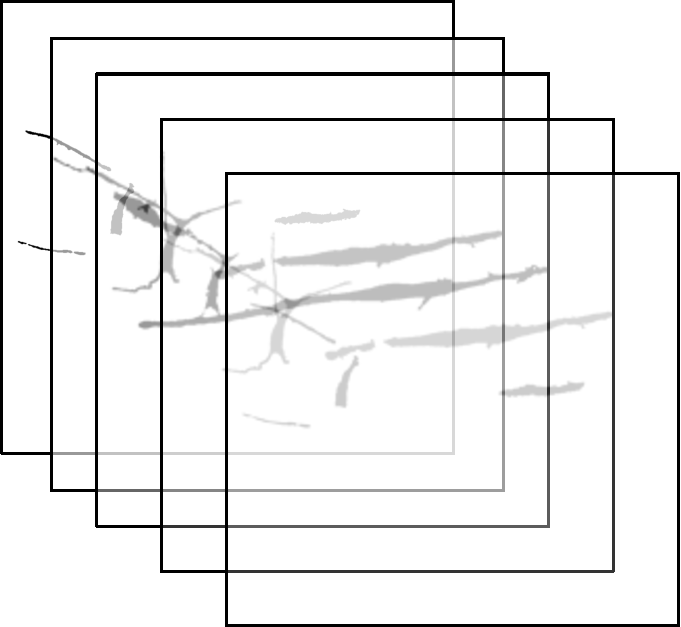
\includegraphics[height=3.5cm]{figure/ImageStack.pdf} & 
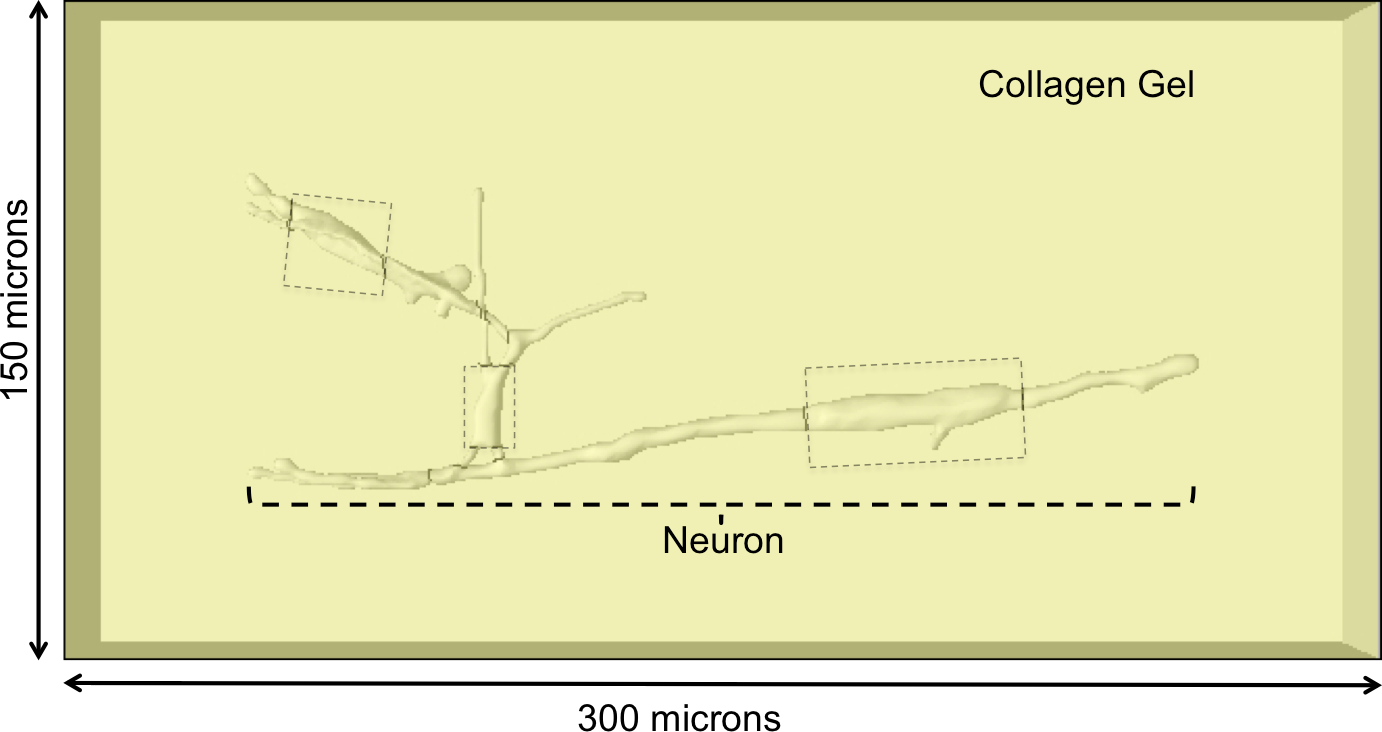
\includegraphics[height=3.5cm]{figure/neuron-in-gel_labels.pdf} &
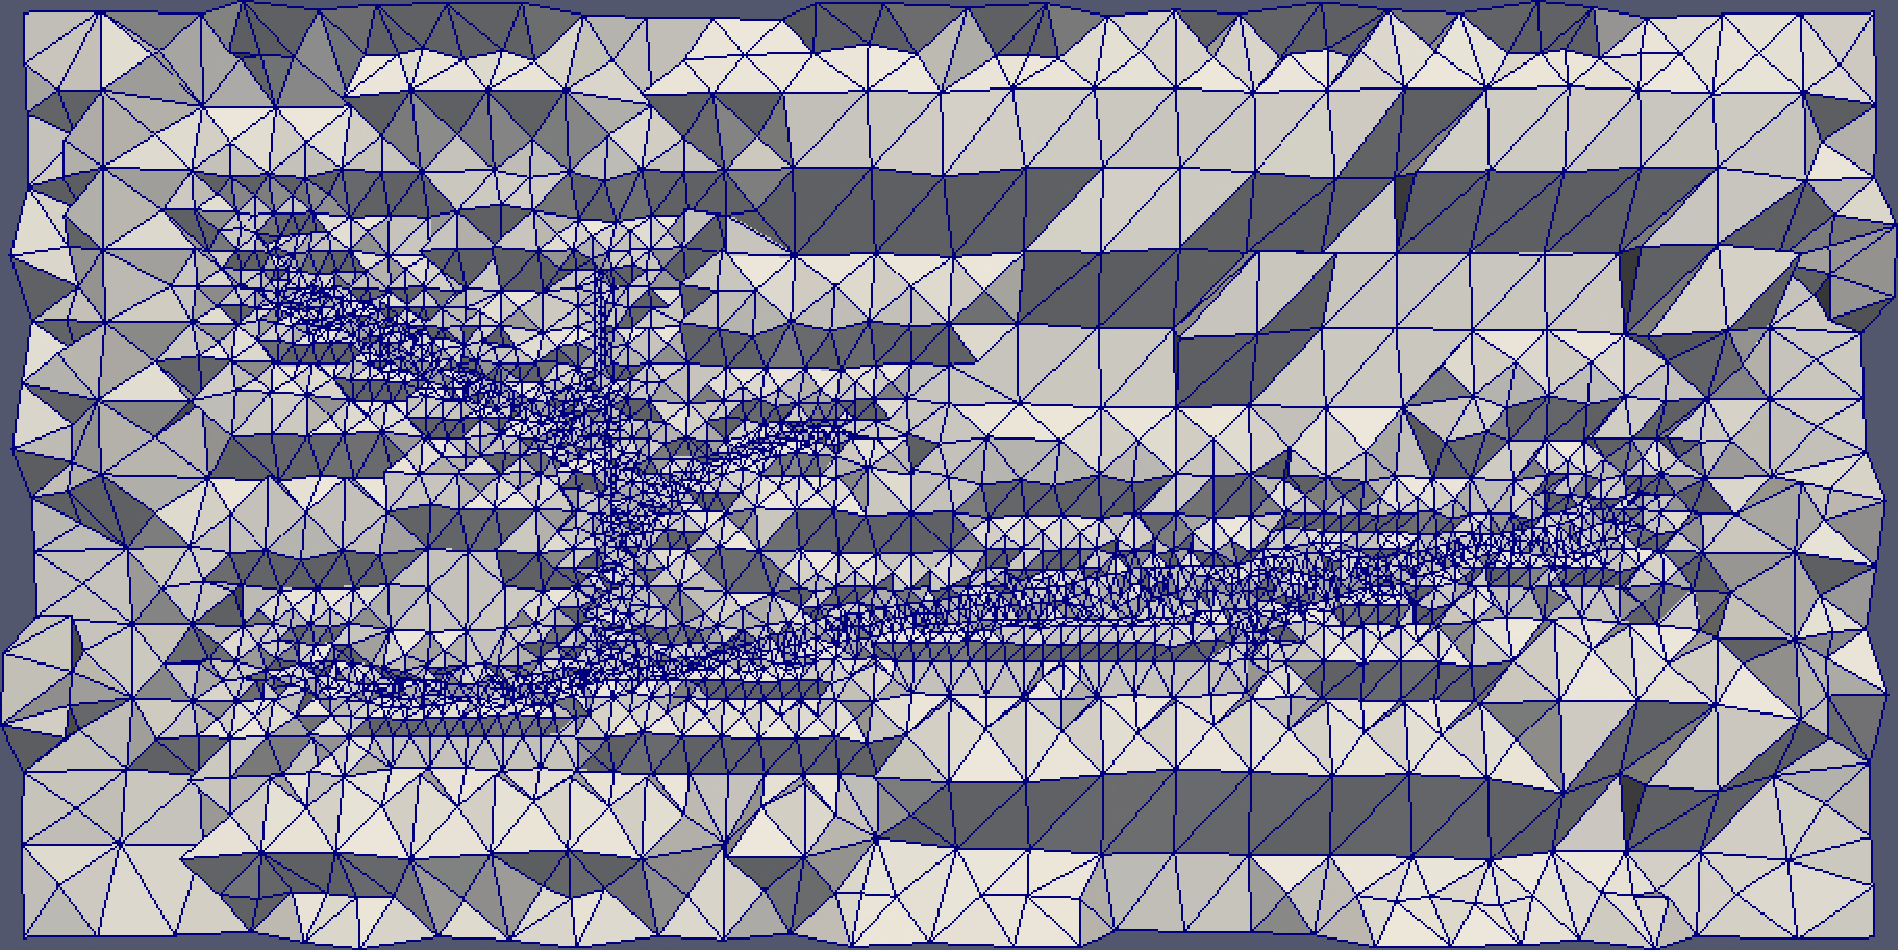
\includegraphics[height=3.5cm]{figure/neuron-in-gel_mesh.pdf} \\
(a) & (b) & (c)
\end{array}
$
\end{center}
\caption{\label{fig:image_to_model} (a) Stack of confocal images of a neuron from neuronal culture. (b) Model of neuron embedded in collagen gel that is generated using the \textit{ImageToModel} tool \cite{Klaas:2013ug, Klaas_conference, simmetrix} from Simmetrix Inc. Regions in the neuron that are marked with dashed rectangles are the cell bodies, while those that are not marked constitute the axons of the neuron. The region enclosing the neuron is the collagen gel. (c) Cut in neuron-in-gel model showing the mesh generated using the SimModeler tool \cite{simmetrix,Shephard:2000vc} from Simmetrix Inc. A mesh of $\sim$80k tetrahedral elements is used for simulations in this work.}
\end{figure}
%

The confocal images were stacked together and converted to a 3D voxelated data set using \textit{ImageJ} \cite{Schneider:2012dw}, where each voxel has dimensions of 0.22$\mu$m $\times$ 0.22$\mu$m $\times$ 2$\mu$m. Voxel data corresponding to different regions of the neuron structure (i.e., axon and cell bodies) were labeled with unique values. Noise arising from the limited level of contrast in the imaging technique and quantization artifacts due to the voxel nature of the data are removed using a combination of erosion/dilation, manual reassignment, small object removal, and smoothing operations which are applied using the \textit{ImageToModel} tool \cite{Klaas:2013ug, Klaas_conference, simmetrix}. The processed voxelated data is converted to a discrete geometry using a marching cube type of procedure \cite{Lorensen:1987vr} which was also applied through the \textit{ImageToModel} tool. Subsequently, the discrete geometric model of the neuron structure was enclosed in a box that represents the domain of the collagen gel, where the neuron-gel interface is perfectly bonded. The mesh of the non-manifold geometry of the embedded neuron structure was generated using the SimModeler tool of Simmetrix Inc. \cite{simmetrix,Shephard:2000vc}. The neuron-in-gel model and its corresponding mesh are shown in Figs.\ \ref{fig:image_to_model}(b) and (c), respectively. 

%=========================================================================================================
\subsection{Multi-Scale Method for Modeling Collagen Gel}
Collagen gel has been modeled in the past using a multi-scale formulation based on volume-averaging of fiber-network representative volume elements (RVEs) \cite{Chandran:2007hy,Stylianopoulos:2007dp,Barocas:2007gk,Lai:2012ji,Lake:2012jm} and is employed to model the collagen gel that surrounds the neuron in our system. The multi-scale formulation consists of two scales: the microscopic scale that represents the fiber level and the macroscopic scale that represents the tissue level. Below, values corresponding to the microscopic and macroscopic scales are denoted with $(m)$ and $(M)$ superscripts, respectively.

The microscopic scale is represented by a collagen network which defines the RVE. Each RVE is generated from a Delaunay triangulation of randomly placed seed points - the edges of the triangulation represent the fibers of the network. Each fiber only carries an axial load where the force on each fiber is given by 
%
\begin{equation}
T_i^{(m)} =
\begin{cases}
\frac{E_f A_f}{B} \left[ \exp(0.5 B(\lambda_f^2 - 1)) - 1\right] & \text{if } \lambda_C \le \lambda_f \le \lambda_S \\
H_C  \lambda_f + h_C & \text{if } \lambda_f \ge \lambda_C \\
H_S \lambda_f + h_S & \text{if } \lambda_f \le \lambda_S
\end{cases}
\label{eq:fiber_force}
\end{equation}
%
where 
%
\begin{align*}
&E_f: \text{linear modulus of a collagen fiber.} \\
&A_f: \text{cross-sectional area of fiber.} \\
&B: \text{constant parameter that controls nonlinearity.} \\
&\lambda_f \equiv \frac{l}{l_0} \text{ where } l \text{ and } l_0 \text{ are the current and initial lengths, respectively, of the fiber. } \\
&\lambda_S: \text{ fiber stretch value at which the fiber relation transitions from nonlinear to linear.} \\
&\lambda_C: \text{ fiber compression value at which the fiber relationship transitions from nonlinear to linear.} \\
&H_i \equiv E_f A_f\lambda_i \exp(0.5B(\lambda_i^2 - 1)) \text{ for } i=S \text{ or } C.\nonumber\\
&h_i \equiv \frac{E_f A_f}{B}\left(\exp(0.5 B (\lambda_i^2-1)-1\right) -H_i \lambda_i \text{ for } i=S \text{ or } C. 
\end{align*}
%
The fiber force shown in Eq.\ \eqref{eq:fiber_force} transitions from a nonlinear to linear relationship when the fiber is stretched beyond $\lambda_S$ or compressed below $\lambda_C$. The transition to a linear fiber force relationship for large fiber stretch is consistent with experimental measurements of single fibers \cite{Eppell:2006hh,Svensson:2010fr}. On the other hand, the transition to a linear fiber force relationship for large fiber compression prevents the RVE from collapsing at large deformations. 

In order to solve for the fiber-force equilibrium in the RVE, displacement boundary conditions are imposed. The displacements at the corners of the RVE are dictated by the deformation state of the macroscopic scale via
%
\begin{equation}
{}^c u^{(m)}_i = (F^{(M)}_{ij} - \delta_{ij}) \frac{{}^c x^{(m)}_j}{L^{(m)}},
\label{eq:downscaling}
\end{equation}
%
where $F^{(M)}_{ij}$ is the deformation gradient tensor of the macroscopic scale, ${}^c u^{(m)}$ are the displacements at the corners of the RVE,  and ${}^c x^{(m)}/L$ are the coordinates at the corners of the RVE. In Eq.\ \eqref{eq:downscaling}, ${}^c x^{(m)}_j$ are coordinates of a dimensionless compute domain that is a cube with sides ranging from -0.5 to 0.5. Therefore, the values of ${}^c x^{(m)}_j$ are either -0.5, 0, or 0.5. The scale conversion, $1/L^{(m)}$, relates the unit lengths between the compute and physical domains. It is important to note that Eq.\ \eqref{eq:downscaling} is valid because the center of the compute RVE is set to lie at the origin of the compute domain. The boundary displacements on each fiber lying on the boundary of the RVE is determined via a linear interpolation. This procedure of determining boundary displacements for the microscopic RVE from the macroscopic deformation state is referred to as \textit{downscaling}. 

Upon solving for fiber-force equilibrium in each RVE, the Cauchy stress tensor for the state at the macroscopic scale are calculated from the forces of fibers that lie on the boundary of the RVE (bcl) \cite{Chandran:2007hy,Stylianopoulos:2007dp}
%
\begin{equation}
\sigma_{ij}^{(M)} = \left(\frac{1}{V^{(m)}} \sum_{\text{bcl}} x_i^{(m)} T_j^{(m)}\right)\left(\frac{1}{L^{(m)}}\right)^2,
\label{eq:macro_stress_discrete}
\end{equation}
%
where $V^{(m)}$ is the current volume of the RVE. The procedure of calculating the macroscopic scale Cauchy stress tensor from microscopic scale equilibrium fiber forces is referred to as \textit{upscaling}. The Cauchy stress tensor obtained from the microscopic scale are used to solve the macroscopic force balance \cite{Chandran:2007hy,Stylianopoulos:2007dp}
%
\begin{equation}
\sigma_{ij,i}^{(M)} = \frac{1}{V^{(m)}} \int_{\partial V^{(m)}} \left( s_{ij}^{(m)} - \sigma_{ij}^{(M)} \right)u_{k,i}^{(m)} n_k dA^{(m)},
\label{eq:macro_stress_divergence}
\end{equation}
%
where $u_k^{(m)}$ is the displacement of the RVE boundary on the microscale, $n_k$ is the unit normal vector, and $s_{ij}^{(m)}$ are elements of the microscopic stress tensor. The right-hand side of Eq.\ \eqref{eq:macro_stress_divergence} acts as a body force that accounts for the correlation between the inhomogeneous displacement of the RVE boundary and local inhomogeneities in the stress field�\cite{Chandran:2007hy,Stylianopoulos:2007dp}. 

%=========================================================================================================
\subsection{Constitutive Relationship for Modeling Neuron}
Cross-linked microtubule bundles that are axially aligned are a major structural feature of axons, giving rise to anisotropic mechanical behavior \cite{Peter:2012fc}. To account for such mechanical anisotropy, the axons are modeled as a transversely isotropic hyperelastic material \cite{JavierBonet:2008uxa,Bonet:1998vc}. The elements of the Cauchy stress tensor and spatial elasticity tensor can be expressed in terms of neo-Hookean (nh) and transversely isotropic (trns) components \cite{Bonet:1998vc}
%
\begin{equation}
\sigma_{ij} = \sigma^{\text{nh}}_{ij} + \sigma^{\text{trns}}_{ij} \ \ \text{ and } \ \ c_{ijkl} = c^{\text{nh}}_{ijkl} + c^{\text{trns}}_{ijkl},
\end{equation}
%
respectively, where 
%
\begin{align}
&\sigma^{\text{nh}}_{ij} = \frac{\mu}{J}(b_{ij} - \delta_{ij}) + \lambda(J-1)\delta_{ij} \nonumber\\
%
&\sigma^{\text{trns}}_{ij} = \frac{2\beta}{J}(a_r a_r - 1)\delta_{ij} + \frac{2}{J}[\alpha+2\beta\ln J+2\gamma(a_r a_r -1)]a_i a_j - \frac{\alpha}{J}(b_{is}a_s a_j+a_i b_{jr}a_r) \nonumber\\
%
&c^{\text{nh}}_{ijkl} = \lambda(2J-1)\delta_{ij}\delta_{kl} + \frac{2}{J}[\mu - \lambda J(2J-1)]\delta_{ik}\delta_{jl} \nonumber\\
%
&c^{\text{trns}}_{ijkl} = \frac{8\gamma}{J}a_i a_j a_k a_l + \frac{4\beta}{J}(a_i a_j \delta_{kl} + \delta_{ij}a_k a_l) - \frac{\alpha}{J}(a_i a_l b_{jk} + b_{ik}a_j a_l) - \frac{4\beta}{J}(a_r a_r - 1)\delta_{ik}\delta_{jl}.
\label{eq:trns_iso}
\end{align}
%
The constants of Eq.\ \eqref{eq:trns_iso} are defined as
%
\begin{align}
&\lambda = \frac{2\mu (\nu+n\nu^2)}{m} \ \ \ \ \ \gamma = \frac{E_A(1-\nu)}{8m} - \frac{\lambda+2\mu}{8} + \frac{\alpha}{2} - \beta \nonumber\\
%
&\alpha = \mu - G_A \ \ \ \ \ \ \ \ \ \ \ \ \ \ m = 1 - \nu - 2 n\nu^2 \nonumber\\
%
&\beta = \frac{\mu \nu^2(1-n)}{2m} \ \ \ \ \ \ \ \ n = \frac{E_A}{2\mu(1+\nu)},
\label{eq:trns_iso_constants}
\end{align}
%
where $\mu$ is the shear modulus, $G_A$ is the axial shear modulus, $\nu$ is the Poisson ratio, and $E_A$ is axial Young's modulus. In our analysis, the shear modulus is set to be isotropic such that $G_A=\mu$ and $\alpha = 0$. All the constants in Eq.\ \eqref{eq:trns_iso_constants} are set once $\mu$, $G_A$, $\nu$, and $E_A$ are specified.

The microtubule bundles transition from an aligned state in the axon to an unaligned state within the cell body \textcolor{red}{[reference describing this phenomenon?]}. To capture such behavior, the cell bodies are also modeled as a transversely isotropic hyperelastic material, however, the axial stiffness is a function of distance from the cell-body/axon interface by
%
\begin{equation}
E_A^{cell} = \left(1 - \frac{D}{a}\right)E_A,
\label{eq:cellEA}
\end{equation}
%
where $D$ is the distance of an interior point of the cell body to the closest cell-body/axon interface and $a$ is a constant that dictates how quickly $E_A$ decreases when moving from the cell-body/axon interface towards the interior of the cell body. The axial stiffness decreases more quickly for smaller values of $a$. According to Eq.\ \eqref{eq:cellEA}, the axial stiffness is lowest at the center of the cell body. 

%%%%%%%%%%%%%%%%%%%%%%%%%%%%%%%%%%%%%%%%%%%%%%%%%%%%%%%%%%%%%%%%%%%%%%
\section{Implementation}
Our model is implemented using the adaptive multi-scale simulation infrastructure (AMSI) \textcolor{red}{[reference for AMSI?]} which is designed to simultaneously handle massively parallel simulations on multiple scales. AMSI enables our model to accommodate the high computational demands that arise from the complex geometry of the neuron structure and the multi-scale nature of the collagen gel. The implementation details are provided below. The choice of modeling parameters in the multi-scale method for the collagen gel and in the constitutive relationship for the neuron are also discussed below.

%=========================================================================================================
\subsection{Adaptive Multiscale Simulation Infrastructure (AMSI)}
\textcolor{red}{Bill can briefly describe implementation of AMSI here.}

%=========================================================================================================
\subsection{Modeling Parameters for Collagen Gel Multi-scale Model}
In the multi-scale method, the scaling parameter $L$ in Eqs.\ \eqref{eq:downscaling} and \eqref{eq:macro_stress_discrete} are required for both the downscaling and upscaling procedures.  The scaling factor $L$ between the compute and physical domains is determined by comparing the average fiber length in the RVEs to that in reconstituted collagen type I networks \cite{Lindstrom:2013gd} with collagen concentration of 2g/L. In the compute domain, fiber networks with a network density (total length of fibers/total number of fibers) of 100 ($\pm$ 1) and an average fiber length 0.26 are used for our RVEs. The average fiber length in reconstituted collagen type I networks is 1.81 $\mu$m \cite{Lindstrom:2013gd}. Based on these average lengths, $L=7 \ \mu$m (1.81 $\mu m$ / 0.26).

As seen in Eq.\ \eqref{eq:fiber_force}, several parameters for the fiber-force relationship must also be specified. The value of $A_f$ is set according to Ref.\ \citenum{Dutov:2016gu} where the fiber radius of rat tail collagen I was measured to be 162 $\mu$m. The values for $E_f$ and $B$ are set by fitting to experimentally measured stress-strain curves of rat tail collagen I gels (see Ref.\ \citenum{Zhang:2016ga} for preparation of collagen samples). To obtain the stress-strain responses experimentally, collagen I gels underwent uniaxial tensile loading at 0.5m/s to 8mm using an Instron 5865 (Instron, Norwood, MA), as described in Ref.\ \citenum{Zhang:2016ga}. The Instron Bluehill software collected the force and displacement data at 1kHz during loading. The stress and strain data are subsequently determined from the force and displacement data by dividing by the initial cross-sectional area and length, respectively, of the sample. 

For $L=7 \mu$m, a good fit to the stress-strain measurements is obtained using the values in Table \ref{table:fiber_parameters} for the parameters in Eq.\ \eqref{eq:fiber_force}.
%%%%%%%%%%%%%%%%%%%%%%%%%%%%%%%%%%%%%%%%%%%%%%%%%%%%%%%%
\begin{table}[ht]
\begin{center}
\begin{tabular}{ l c  }
\hline \hline
$E_f:$ & 200 kPa \\
$B:$ & 20 \\
$\lambda_S:$ &1.13 \\
$\lambda_C:$ & 0.0 \\ \hline \hline
\end{tabular}
\end{center}
\caption{Parameters for fiber force relationship in Eq.\ \eqref{eq:fiber_force}.}
\label{table:fiber_parameters}
\end{table}
%%%%%%%%%%%%%%%%%%%%%%%%%%%%%%%%%%%%%%%%%%%%%%%%%%%%%%%%
%
The fiber force for the parameters listed in Table \ref{table:fiber_parameters} is plotted in Fig.\ \ref{fig:stress_strain}(a). The stress-strain curves calculated from simulation (using Eq.\ \eqref{eq:fiber_force}) and measured experimentally are shown in Fig.\ \ref{fig:stress_strain}(b).
%
% (a) stress-strain curve from N2P178/1-NewParams_Cube/stress-strain folder.
% (b) fiber force curve from N2P177/LRT_Compression folder.
\begin{figure}[ht]
\begin{center}
$
\begin{array}{cc}
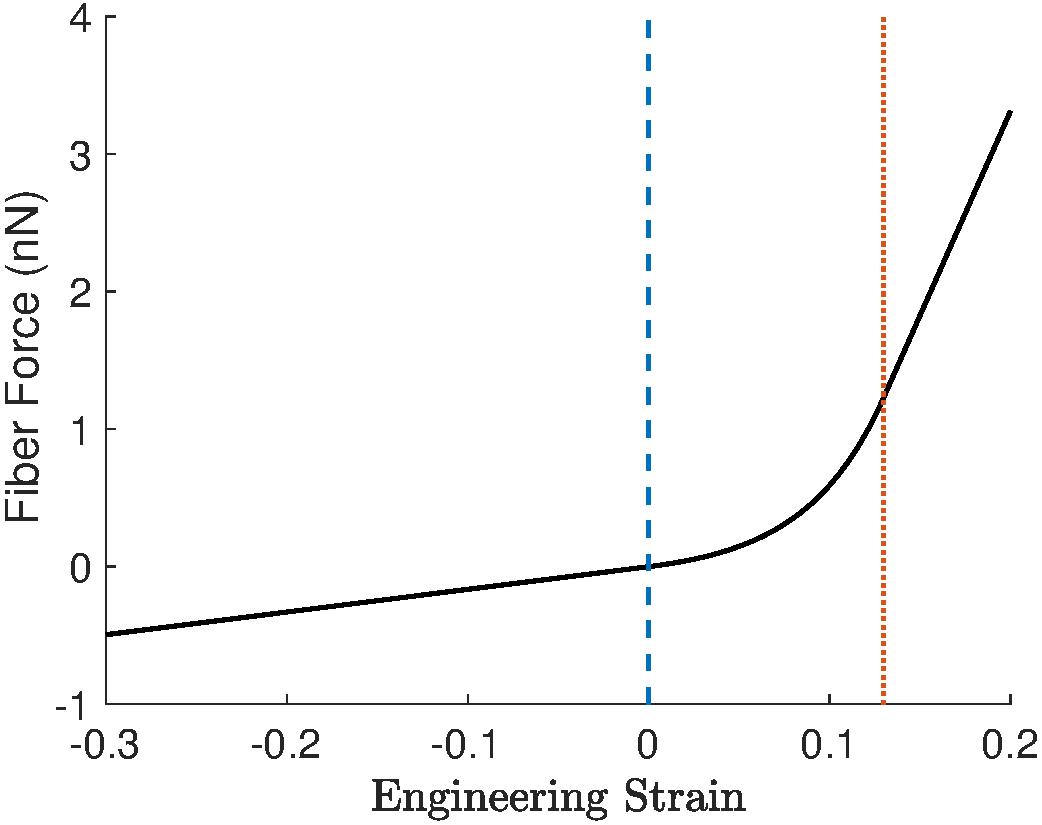
\includegraphics[height=5cm]{figure/FiberForceRelation.pdf} &
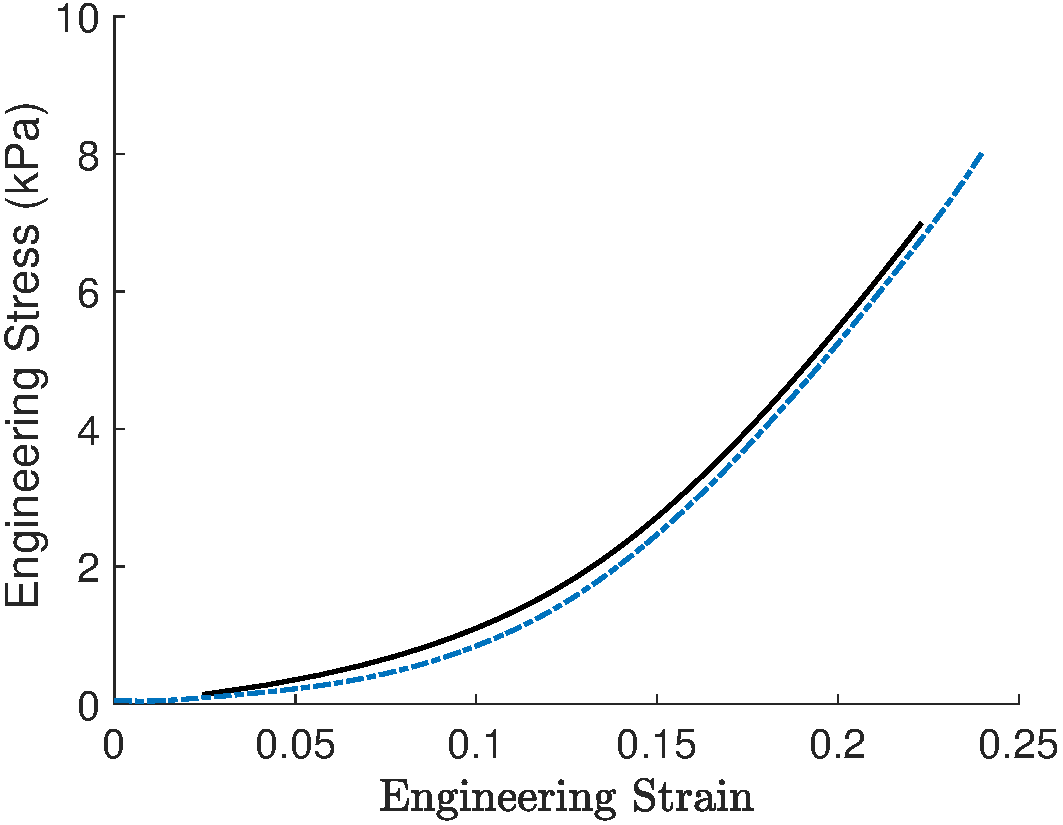
\includegraphics[height=5cm]{figure/stress_strain.pdf} \\
(a) & (b) 
\end{array}
$
\end{center}
\caption{\label{fig:stress_strain} Plots of (a) fiber-force relationship for RVEs used in the simulation (blue ``x"), and (b) stress-strain curve calculated from simulation (blue ``x'') and measured experimentally (black line). The parameters of the fiber-force relationship are listed in Table \ref{table:fiber_parameters}. The stiffness in tension and compression in the linear fiber-force regimes are 29.7 kPa and 1.65 kPa, respectively. }
\end{figure}
%

The Poisson ratio is measured from the volume change of the domain via
%
\begin{equation}
\nu = \frac{1}{2}\left(1- \frac{\Delta V}{V_0}\frac{l_0}{\Delta l}\right).
\label{eq:poisson-ratio}
\end{equation}
%
The Poisson ratio as a function of applied bulk strain for the fiber-force parameters listed in Table.\ \ref{table:fiber_parameters} is plotted Fig.\ \ref{fig:fiber_param2}(a). The Poisson ratio increases as a function of applied strain, and becomes larger than 0.5 at an applied strain of approximately $17\%$. The increasing Poisson ratio at larger applied strains is due to the densification of the fiber network \cite{Vader:2009js} where the fibers in the RVE become increasingly aligned. At lower strains, the increasing Poisson ratio is due to the nonlinear fiber-force relationship where the stiffness in tension is increasing (see stress-strain curve in Fig.\ \ref{fig:stress_strain}).
%
% (a) Poisson ratio curve from N2P178/1-NewParams_Cube/poisson-ratio folder.
% (b) Alignment curve from N2P178/1-NewParams_Cube/alignment folder.
\begin{figure}[ht]
\begin{center}
$
\begin{array}{cc}
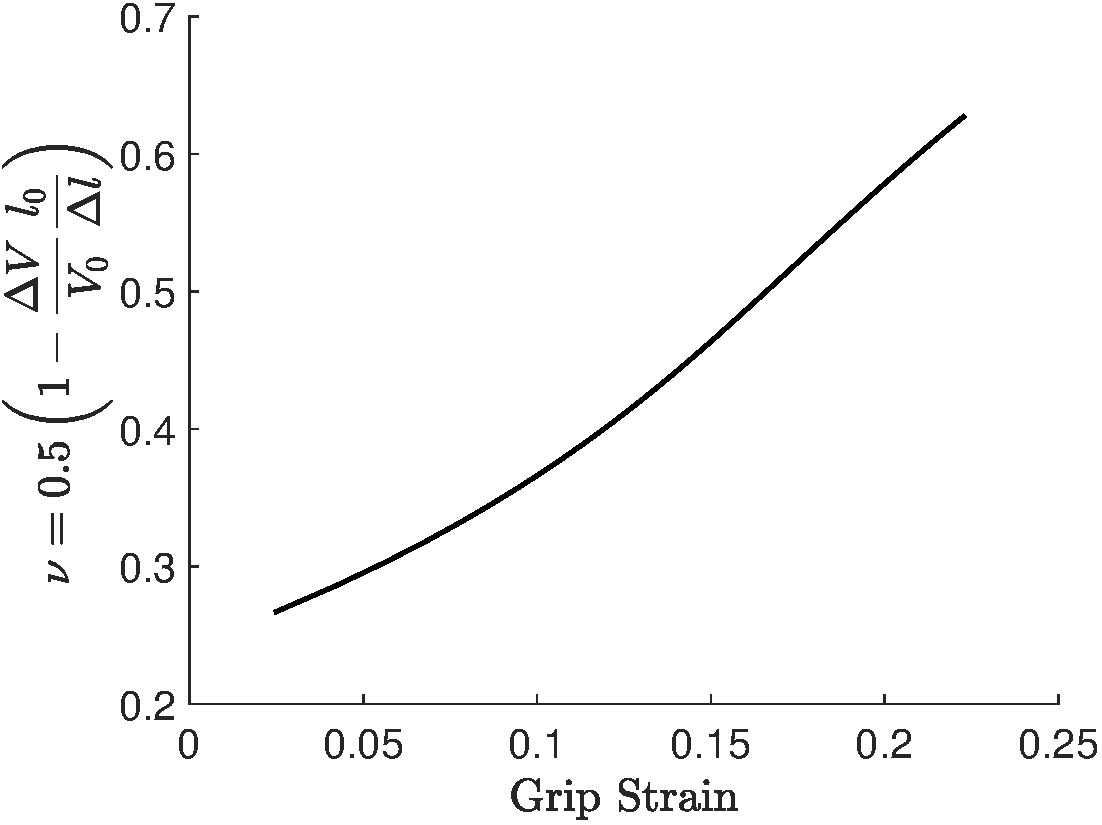
\includegraphics[height=5cm]{figure/PoissonRatio.pdf} &
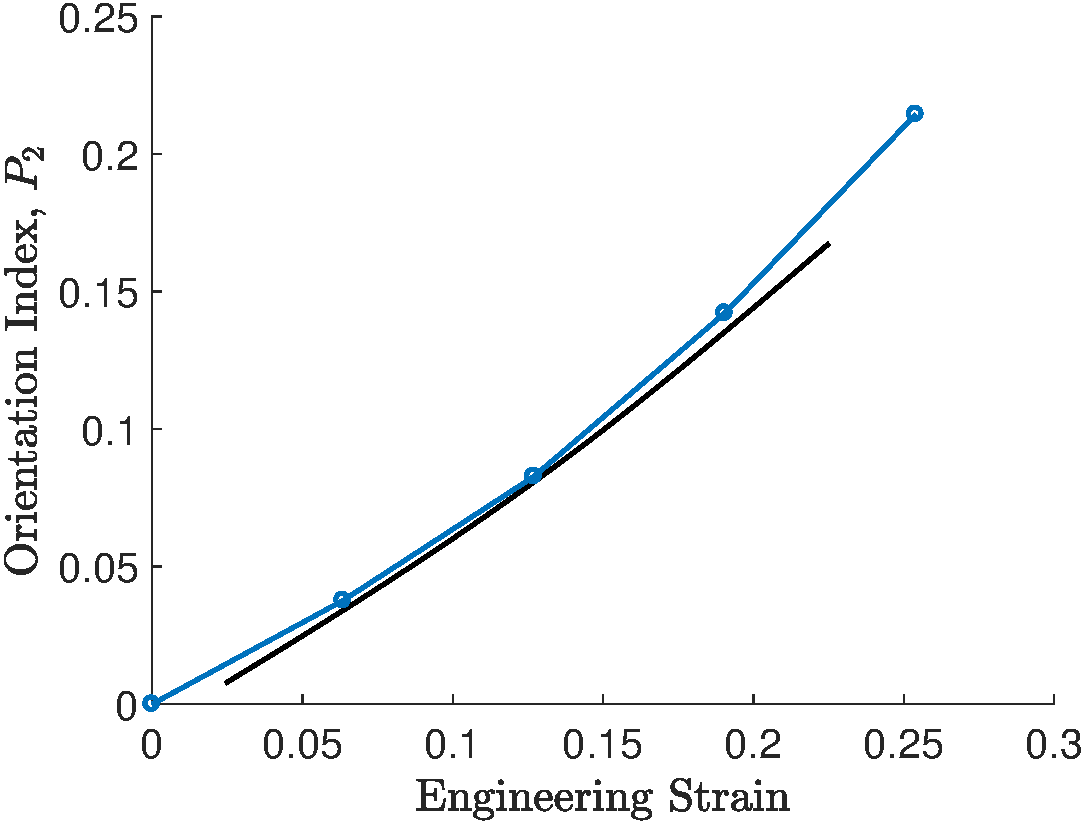
\includegraphics[height=5cm]{figure/alignment.pdf} \\ 
(a) & (b)
\end{array}
$
\end{center}
\caption{\label{fig:fiber_param2} Plots of (a) Poisson ratio calculated from simulation and (b) fiber alignment metric $P_2$ calculated from simulation (blue ``x") and measured experimentally (black line). Simulation results are calculated using fiber parameters listed in Table \ref{table:fiber_parameters}.}
\end{figure}
%

The fiber alignment in innervated collagenous tissue was measured using the QPLI method \cite{Quinn:2008df,Quinn:2009bf} where alignment angle $\alpha$ and retardation $\delta$ is measured in each pixel. Our customized QPLI system is comprised of a fiber-optic light source (Dolan-Jenner Industries Inc., Boxborough, MA), a motor-controlled linear polarizer (Edmund Optics, Barrington, NJ) that rotates at 750 rpm, and a circular analyzer mounted to a high-speed camera (Phantom-v9.1; Vision Research Inc, Wayne, NJ) \cite{Zhang:2016ga}. The QPLI system was integrated with the mechanical testing device, and collagen I gels were placed between the rotating polarizer and the circular analyzer. Polarized light images were acquired during tensile loading at 500 fps with 14.5 pixel/mm resolution and processed using harmonic analysis to extract the alignment angle and retardation \cite{Tower:2002hk,Quinn:2008df}. To compare fiber alignment that is measured experimentally and calculated from simulations, the orientation index $P_2$ is considered. The value of $P_2$ is calculated from the angle $\theta$ between fibers and the direction of alignment
%
\begin{equation}
P_2 = \frac{3 <\cos^2\theta> - 1}{2},
\label{eq:P2_simulation}
\end{equation}
%
where $<a>$ denotes the average of $a$. The value of $P_2$ ranges from 1 ($\theta=0$ or $\pi$) in which the fibers are completely aligned to -1/2 ($\theta=\pi/2$) in which the fibers are orthogonal to the alignment direction. When $P_2=0$, the fiber network is randomly oriented. The orientation index $P_2$ can be calculated from $\alpha$ and $\delta$ of the QPLI method via \textcolor{red}{[see Appendix for derivation]}
%
\begin{align}
&P_2 = \int_0^{\pi} p(\theta) \cos^2\theta d\theta \nonumber\\
&p(\theta) = \frac{1}{N} \sum_{i=1}^N \left[ \frac{1-2\delta_i}{\pi} + \frac{4 \delta_i}{\pi}\cos^2(\theta - \alpha_i)\right],
\label{eq:P2_experiment}
\end{align}
%
where $\delta_i$ and $\alpha_i$ are the retardation and alignment angle, respectively, of the $i^{th}$ pixel. The fiber alignment as a function of bulk applied strain calculated from simulation and measured experimentally are plotted in Fig.\ \ref{fig:fiber_param2}(b). \textcolor{red}{[According to Professor Picu, alignment is more pronounced at low strains and less pronounced at high strains if deformation is non-affine (compared to the case of affine deformation). The behavior in Fig.\ \ref{fig:fiber_param2}(b) is in agreement if it is valid that the Delaunay fiber network that we are using deforms affinely due to the the large coordinate of the Delaunay network used in our model.]}

%=========================================================================================================
\subsection{Model Parameters for Neuron Constitutive Relationship}
To model the neuron with Eq.\ \eqref{eq:trns_iso}, several parameters in the relationship must be specified. The value of $E_A$ is based on the study by Peter and Mofrad \cite{Peter:2012fc}, where the mechanical behavior of axonal microtubule bundles under tension were simulated with a discrete bead-spring model. \textcolor{red}{Since microtubule bundles are the stiffest...} To apply their results for microtubule bundles to our neuron model, we assume that only the microtubule bundles carry force in the axon and that the stress of the microtubule bundles can be redistributed over the cross-sectional area of the axon. \textcolor{red}{[Here we assume that the contribution from the membrane cortex (filamin) is negligible)].} Based on these assumptions, the axial stiffness of the axon can be related to the axial stiffness of the microtubule bundles, $E_{MTb}$, by
%
\begin{equation}
E_A = \frac{E_{MTb} A_{MTb}}{A_A},
\label{eq:EA_EMTb_relation}
\end{equation}
%
where $A_{MTb}$ and $A_A$ are the cross-sectional areas of the microtubule bundle and axon, respectively. Peter and Mofrad \cite{Peter:2012fc} showed that the stress-strain relationship of the microtubule bundle is well represented by a power-law fit which results in an elastic modulus that is a function of strain. For our study, $E_{MTb}$ is taken to be an average value of $4\times 10^{4}$ kPa. The cross section of the microtubule bundle is schematically shown in Fig.\ \ref{fig:microtubule_bundle}, from which $A_{MTb}$ is determined to be 0.344 $\mu$m${}^2$. 
%
%image from BiotissueMeetings/Biotissue_Meeting_3_17_17
\begin{figure}[ht]
\begin{center}
$
\begin{array}{c}
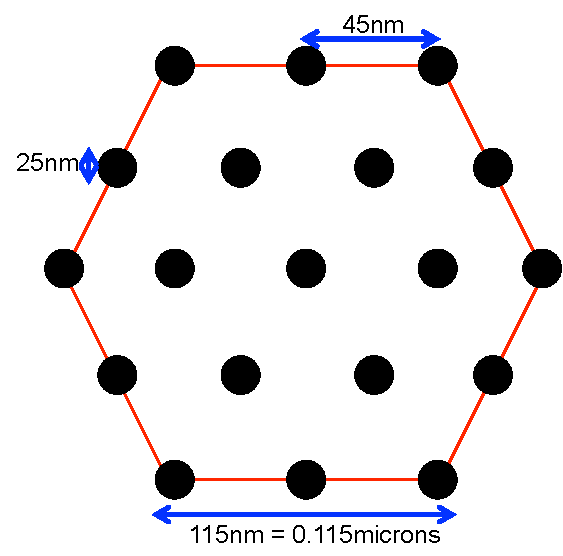
\includegraphics[height=5cm]{figure/microtubule_bundle.pdf} 
\end{array}
$
\end{center}
\caption{\label{fig:microtubule_bundle} Cross-section of microtubule bundle based on dimensions from Ref.\ \citenum{Peter:2012fc}. Diameter of a microtubule (black dot) is 25nm and edge-to-edge spacing between microtubules is 20nm. Figure is not drawn to scale. }
\end{figure}
%
The average axon diameter of the neuron structure is approximately 5 $\mu$m, from which $A_A$ is determined to be 19.6 $\mu$m${}^2$. Based on the above values, $E_A$ is determined from Eq.\ \eqref{eq:EA_EMTb_relation} to be 70 kPa. The parameters used in Eq.\ \eqref{eq:trns_iso_constants} for modeling the neuron structure are listed in Table \ref{table:neuron_parameters}. 
%%%%%%%%%%%%%%%%%%%%%%%%%%%%%%%%%%%%%%%%%%%%%%%%%%%%%%%%
\begin{table}[ht]
\begin{center}
\begin{tabular}{ l l }
\hline \hline
$E_A = $ 70 kPa  & axial elastic modulus calculated from Eq.\ \eqref{eq:EA_EMTb_relation}. \\ 
$E_T = $ 1.5 kPa & transverse elastic modulus. \\
$\nu = $ 0.3 & Poisson ratio. \\
$\mu = $ 0.577 kPa & shear modulus calculated from $E_T$ and $\nu$. \\ 
$G_A = \mu = $ 0.577 kPa & axial shear modulus.\\ \hline \hline
\end{tabular}
\end{center}
\caption{Parameters of Eq.\ \eqref{eq:trns_iso_constants} for modeling neuron structure. The transverse elastic modulus, $E_T$, is based on measurements of the neuron cell body by Simon et al.\ \cite{Simon:2016ig}. The shear modulus of the neuron structure is assumed to be isotropic. Therefore, $G_A = \mu = 0.577$ kPa.}
\label{table:neuron_parameters}
\end{table}
%%%%%%%%%%%%%%%%%%%%%%%%%%%%%%%%%%%%%%%%%%%%%%%%%%%%%%%%

%%%%%%%%%%%%%%%%%%%%%%%%%%%%%%%%%%%%%%%%%%%%%%%%%%%%%%%%%%%%%%%%%%%%%%
\section{Results}
\label{sec:Results}

The embedded neuron model described above is used to examine the local biomechanical mechanisms that give rise to neuron injury. Our model of a single embedded neuron enables the examination of local strain concentrations that develop within the neuron when the surrounding collagen gel is deformed. \textcolor{red}{[How representative is this one neuron configuration that we study? Can we extrapolate these results to other studies?]} These results provide physiological insights about the mechanisms that give rise to pain when an innervated ligament is excessively loaded.

In our simulations, the collagen gel surrounding the neuron structure is deformed to bulk (far field) strains of up to 16$\%$, which corresponds to painful ligament loading \cite{Zhang:2016ga}. The strain within the neuron structure is quantified by a complementary cumulative distribution function (ccdf) defined as 
%
\begin{equation}
1 - \text{cdf}(X) = 1 - \sum_{i<X} f(i) = \text{Pr}[ \epsilon_{\text{max}}/\epsilon_{\text{bulk}} \le X],
\label{eq:ccdf}
\end{equation}
%
where $f$ is the probability density function of the maximum principal strain (MPS) that is normalized by the the applied bulk strain on the surrounding gel, $\epsilon_{\text{max}}/\epsilon_{\text{bulk}}$, and $X$ is a specific value of the normalized MPS. A normalized MPS that is greater than unity indicates that the applied bulk strain on the surrounding collagen gel is amplified in the neuron structure. When the local-strain amplification is large, moderate loads that are applied to the surrounding gel can give rise to injury in the neuron. Equation \ref{eq:ccdf} is the probability that the neuron structure (equivalent to the volume fraction of the neuron) experiences a local-strain amplification of \textit{at least} $X$. 

%=========================================================================================================
\subsection{Strain Distribution}
In this section, we examine the MPS of an embedded neuron structure that is loaded at 0 degrees. Different loading cases on the collagen gel are shown schematically in Fig.\ \ref{fig:analysis_schematic}(a). The axial stiffness in the cell body, $E_A^{\text{cell}}$, is described by Eq.\ \eqref{eq:cellEA} with $a=30$. According to Eq.\ \eqref{eq:cellEA}, $E_A^{\text{cell}}$ depends on $D$, which is the nearest distance from the cell-body/axon interface. As seen in Fig.\ \ref{fig:analysis_schematic}(b), the largest cell body in the neuron has an axial length of approximately 51 $\mu$m, which gives $D = 25.5 \ \mu$m. Based on these values, $E_A^{\text{cell}}$ at the center of the largest cell is determined by Eq.\ \eqref{eq:cellEA} to be 10.5 kPa, which is consistent with the axial stiffness color map plotted in Fig.\ \ref{fig:analysis_schematic}(b).  
%
%image for axial young's modulus from N2P178/3-Neuron_FT folder
\begin{figure}[ht]
\begin{center}
$
\begin{array}{cc}
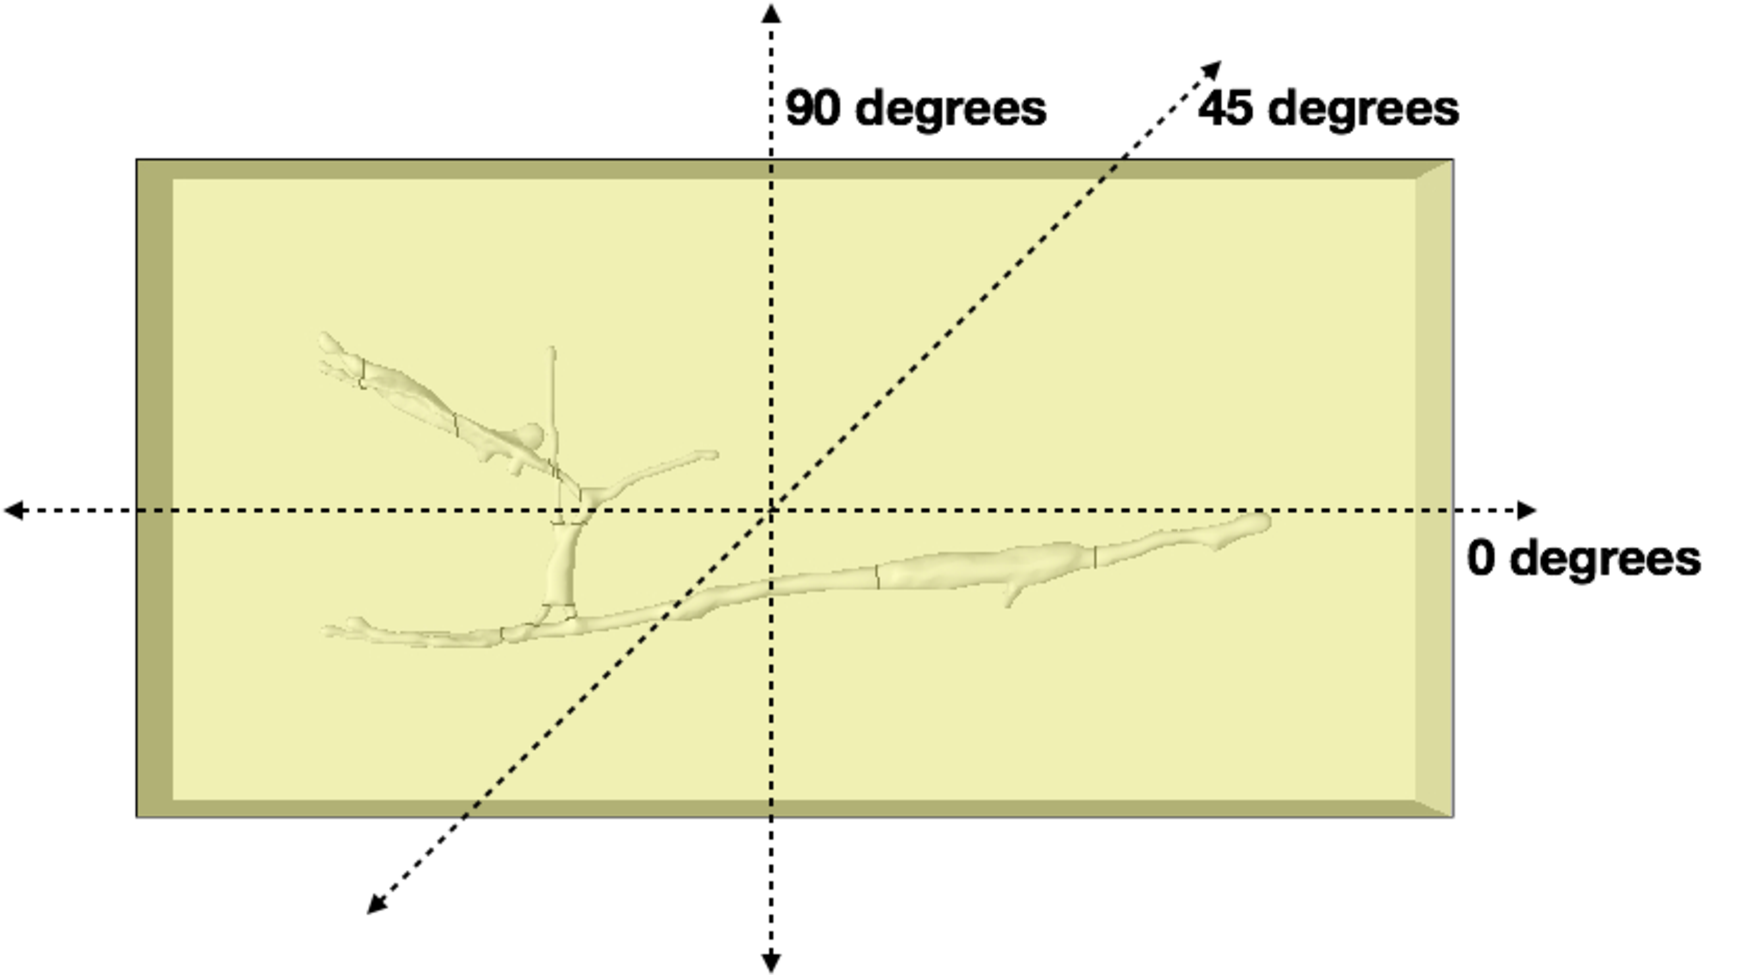
\includegraphics[height=4cm]{figure/AngleLoadingSchematic.pdf} &
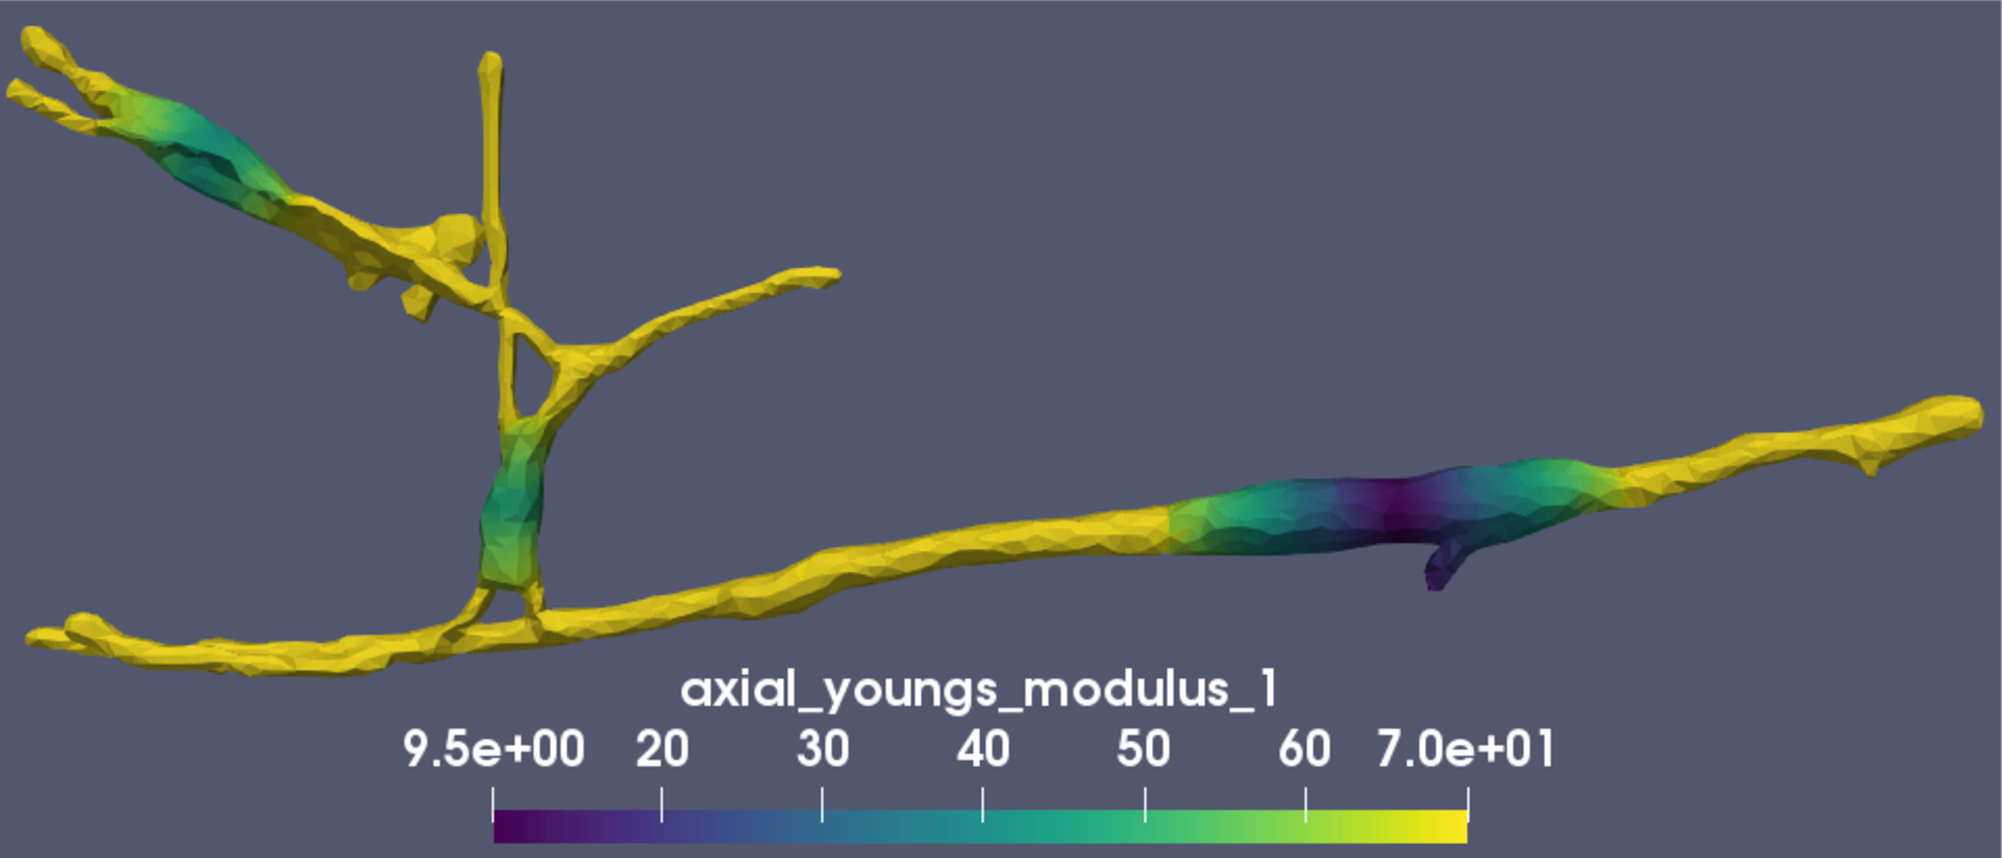
\includegraphics[height=3.5cm]{figure/axial_youngs_modulus_a30.pdf} \\
(a) & (b)
\end{array}
$
\end{center}
\caption{\label{fig:analysis_schematic} (a) Schematic showing axes of load directions corresponding to 0, 45, and 90 degrees. (b) Plot of axial Young's modulus for $a=30$ in Eq.\ \eqref{eq:cellEA} and $E_A=70$ kPa.}
\end{figure}
%

Color maps of the MPS on the neuron structure for bulk strains of 10$\%$ (non painful ligament loading) and 16$\%$ (painful ligament loading) in the collagen gel are plotted in Fig.\ \ref{fig:neuron_0deg_MPS}.
%
% Images from N2P178/4-Neuron_FT_trcBC folder.
\begin{figure}[ht]
\begin{center}
$
\begin{array}{cc}
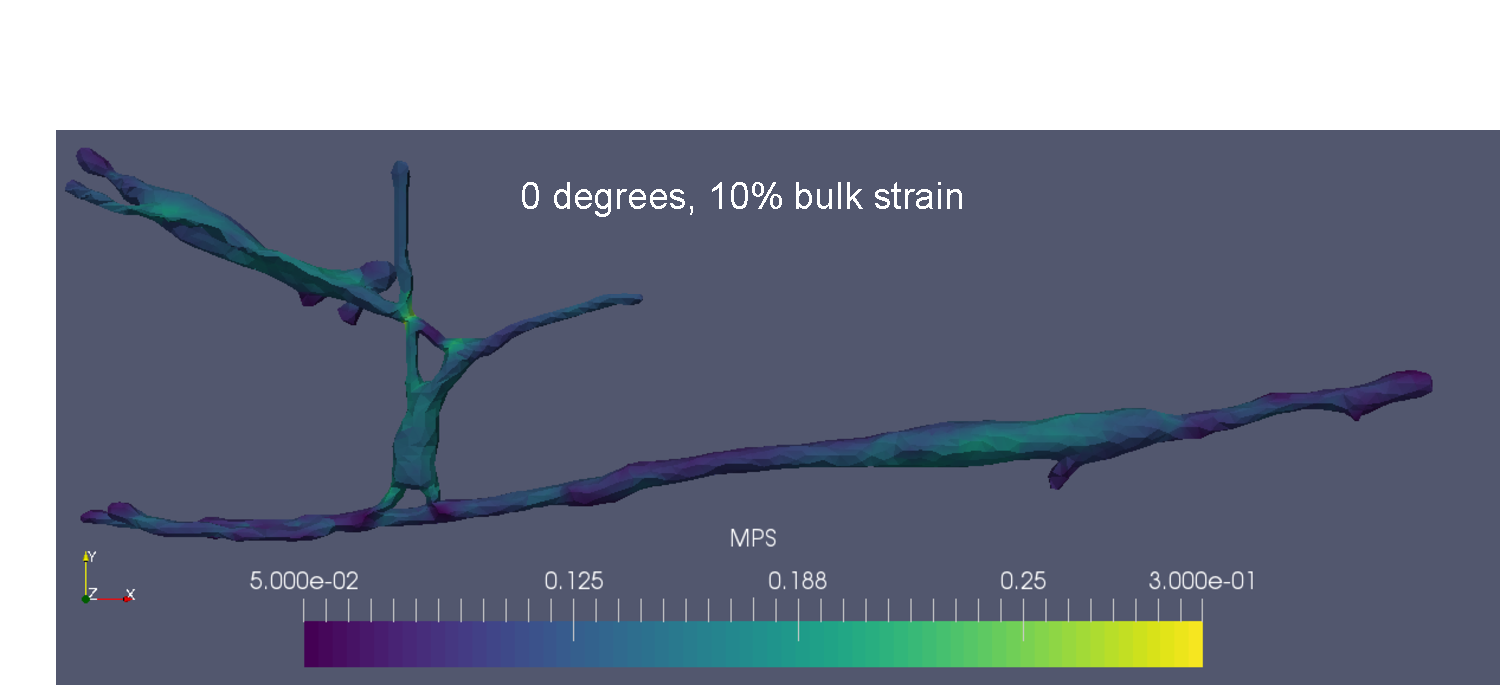
\includegraphics[height=3.25cm]{figure/MPS_rot0_strain10.pdf} & 
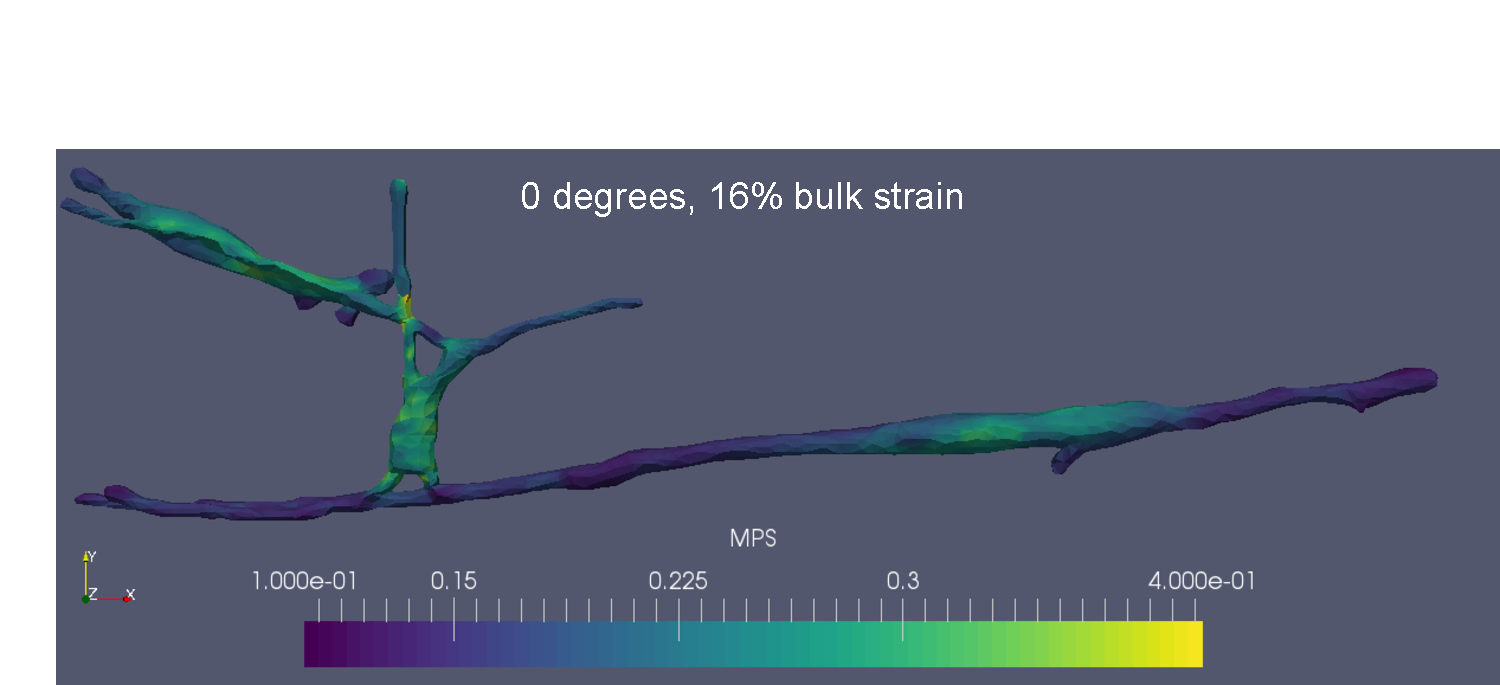
\includegraphics[height=3.25cm]{figure/MPS_rot0_strain16.pdf} \\
(a) & (b) 
\end{array}
$
\end{center}
\caption{\label{fig:neuron_0deg_MPS} Color maps of MPS plotted on neuron structure for loading angle of 0 degrees for bulk strains of (a)10$\%$ and (b) 16$\%$ in the collagen gel. The axial stiffness in the cell body is described by Eq.\ \eqref{eq:cellEA} with $a=30$. Note that the color bar ranges from 5$\%$ to 30$\%$ strain for bulk strain of 10$\%$ and from 10$\%$ to 40$\%$ for 16$\%$ bulk strain.}
\end{figure}
%
For both non painful and painful ligament loading, large portions of the neuron experience strains that are greater than the applied bulk strain on the surrounding gel. This indicates that the applied strains on the collagen gel are amplified in the neuron structure, which can lead to neuronal damage even when the surrounding tissue is moderately loaded. 

To gain a more quantitative understanding of the local-strain amplification in the neuron, ccdfs of the normalized MPS in the neuron are plotted in Fig.\ \ref{fig:neuron_ccdf_0deg_mps} for 10$\%$ and 16$\%$ bulk strains in the collagen gel.
%
% Figures generated in N2P178/4-Neuron_FT_trcBC/MaxPrnStrn folder
\begin{figure}[ht]
\begin{center}
$
\begin{array}{cc}
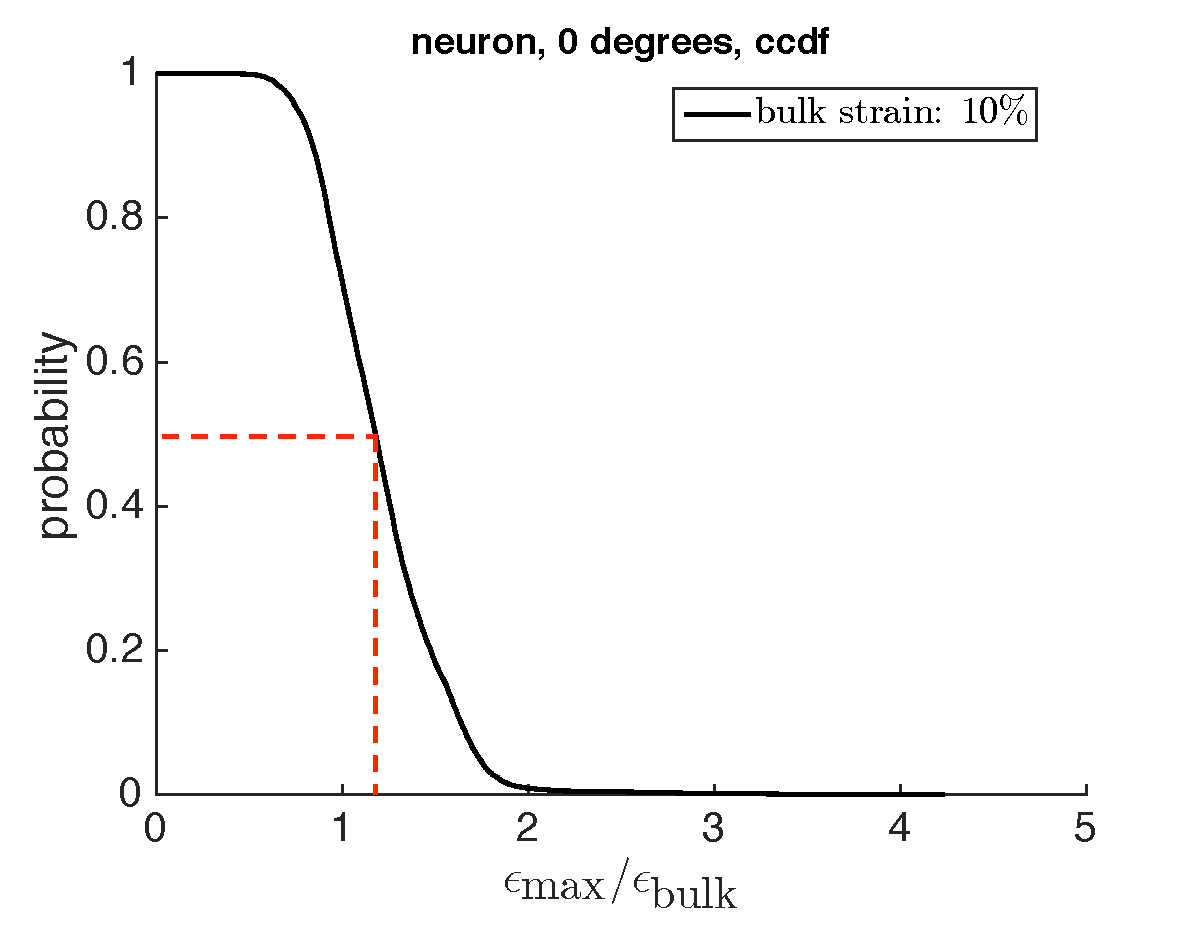
\includegraphics[height=6cm]{figure/neuron_0deg_MPS_ccdf_10.pdf} &
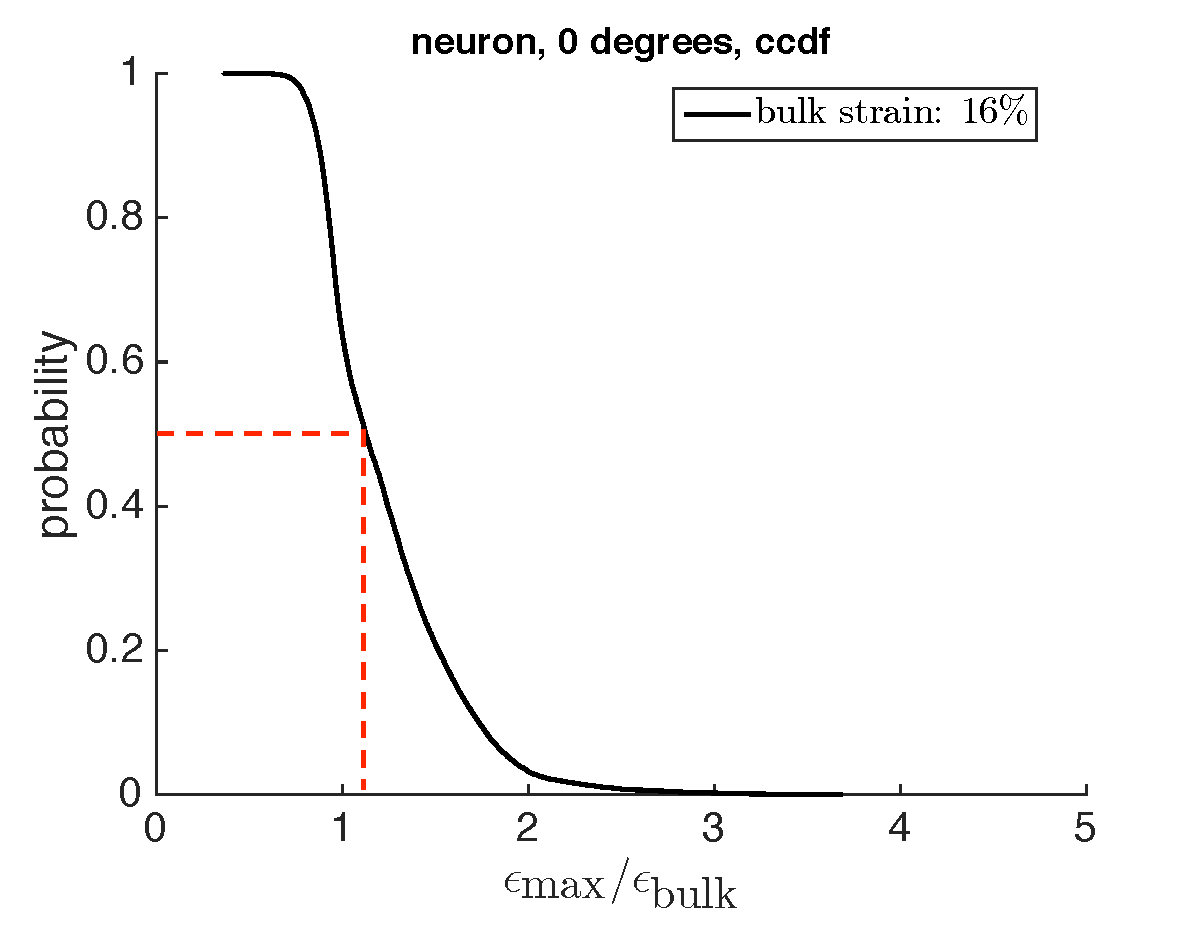
\includegraphics[height=6cm]{figure/neuron_0deg_MPS_ccdf_16.pdf} \\
(a) & (b) 
\end{array}
$
\end{center}
\caption{\label{fig:neuron_ccdf_0deg_mps} ccdfs of normalized MPS in the neuron for bulk strains of (a) 10$\%$ and (b) 16$\%$ in the collagen gel. The averages (50$\%$ probability) are indicated by the dashed red lines. }
\end{figure}
%
For both non painful and painful ligament loading, the average normalized MPS in the neuron structure is greater than unity. In both cases, portions of the neuron experience local-strain amplification of more than three times the applied bulk strain. These results quantitatively capture what is observed in the color maps of Fig.\ \ref{fig:neuron_0deg_MPS}.

%=========================================================================================================
\subsection{Effect of Changing the Axial Stiffness in the Cell Body}
\label{sec:cellbody_stiffness}
In our model, the axial stiffness of the cell body depends on how quickly the microtubules in the neuron transition from an aligned state in the axon to an unaligned state in the cell body. The transition from the aligned to unaligned state is characterized by the variable $a$ in Eq.\ \eqref{eq:cellEA}. To explore the effect of such a transition on the overall mechanical behavior of the neuron, the value of $a$ in Eq.\ \eqref{eq:cellEA} is adjusted. A larger value of $a$ represents a more rapid transition from the aligned to unaligned state and results in an overall softer cell body. 

As seen in Eq.\ \eqref{eq:cellEA}, the value of $a$ needs to be greater than $D$, which is 25.5 $\mu$m in order for $E_A^{\text{cell}}$ to be positive. In this section three values of $a$ are considered: $a=$ 28 $\mu$m, 30 $\mu$m, and 50 $\mu$m, which correspond to axial stiffnesses of approximately 6.25 kPa, 10.5 kPa, and 34.3 kPa, respectively, at the center of the largest cell body in the neuron. The ccdfs for different axial stiffnesses of the cell body (different values of $a$) are plotted in Fig.\ \ref{fig:neuron_ccdf_vary_a} for the 0 degree loading case at an applied bulk strain of 16$\%$ in the collagen gel. 
%
% Figures generated in N2P178/6-Neuron_CellStiffness/MaxPrnStrn folder
\begin{figure}[ht]
\begin{center}
$
\begin{array}{c}
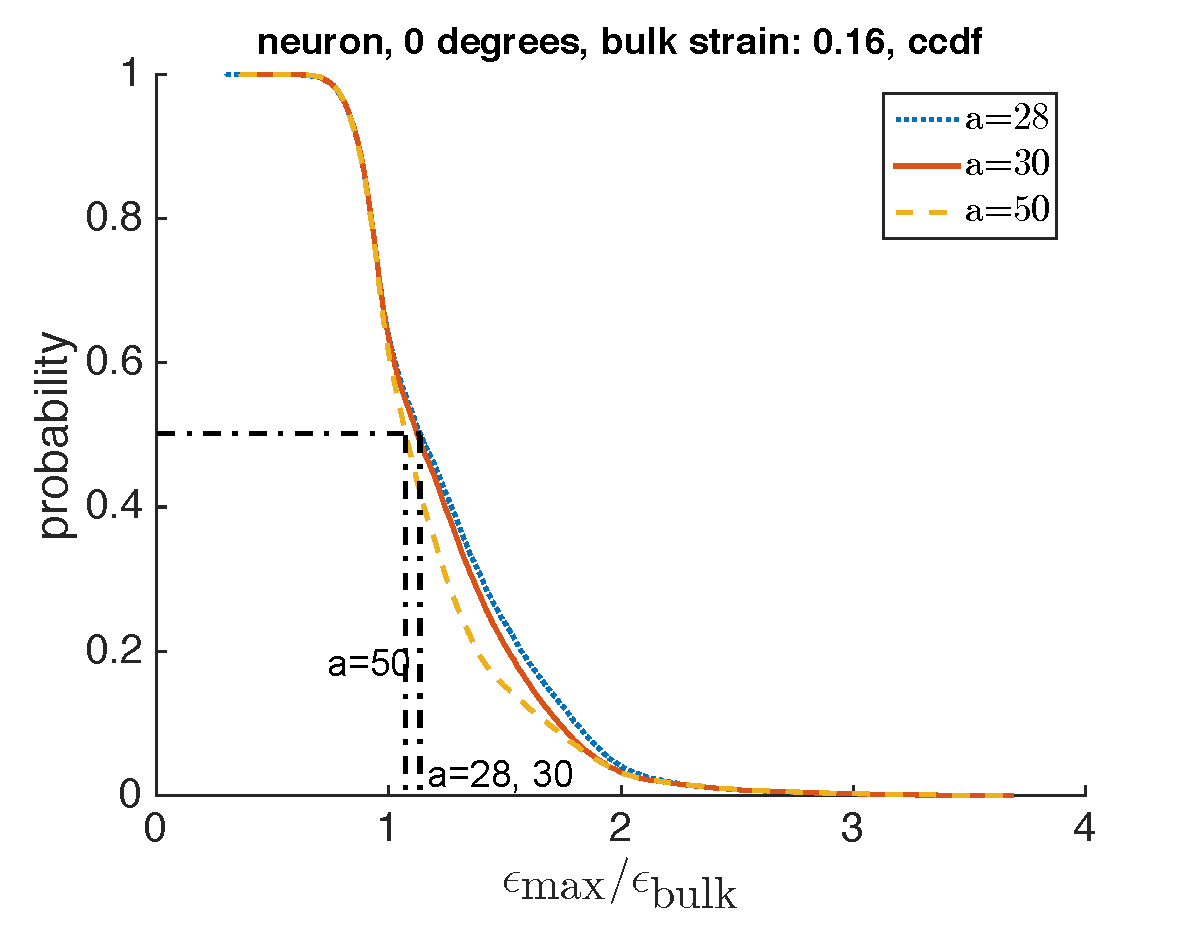
\includegraphics[height=8cm]{figure/neuron_compare_a_ccdf.pdf} 
\end{array}
$
\end{center}
\caption{\label{fig:neuron_ccdf_vary_a} ccdfs of normalized MPS in neuron structure for axial stiffnesses of cell body corresponding to a=28 (blue dotted line), 30 (red solid line), and 50 (dashed yellow line). The averages are indicated with black dashed-dotted lines. }
\end{figure}
%

As seen in Fig.\ \ref{fig:neuron_ccdf_vary_a}, the volume fraction of the neuron that experiences a normalized MPS of less than unity remains constant for all values of $E_A^{\text{cell}}$ considered. On the other hand, the volume fraction of the neuron that experiences a normalized MPS of greater than unity decreases only slightly as $E_A^{\text{cell}}$ increases. On average, the normalized MPS for all values of $E_A^{\text{cell}}$ considered is greater than unity, with portions of the neuron that experience local-strain amplifications of more than three times. The small effect that changing $E_A^{\text{cell}}$ has on the overall strain distribution of the neuron suggests that the local-strain amplification experienced in the embedded neuron structure is not due to variations in its material properties. Therefore, the effect of the configuration of neuron structure relative to loading direction is explored in the next section.

%=========================================================================================================
\subsection{Effect of Changing the Loading Direction}
\label{sec:loading_direction}
In this section, we examine how the ccdf of the neuron structure changes when the loading direction on the collagen gel is varied. The structural features in the neuron are exposed to different modes of deformation when the loading direction is adjusted. Through this analysis, we hope to gain insights about how the geometric configuration of the neuron can give rise to local-strain amplification.

The three different loading cases considered in this section are schematically shown in Fig.\ \ref{fig:analysis_schematic}(a). The effect of changing the loading angle is explored for $E_A^{\text{cell}}$ corresponding to $a$=30 in Eq.\ \eqref{eq:cellEA}. Color maps of the MPS on the neuron structure for loading angles of 45 and 90 degrees are plotted in Fig.\ \ref{fig:neuron_MPS} for bulk strains of 10$\%$ and 16$\%$ in the collagen gel.
%
% Images from N2P178/4-Neuron_FT_trcBC folder.
\begin{figure}[ht]
\begin{center}
$
\begin{array}{cc}
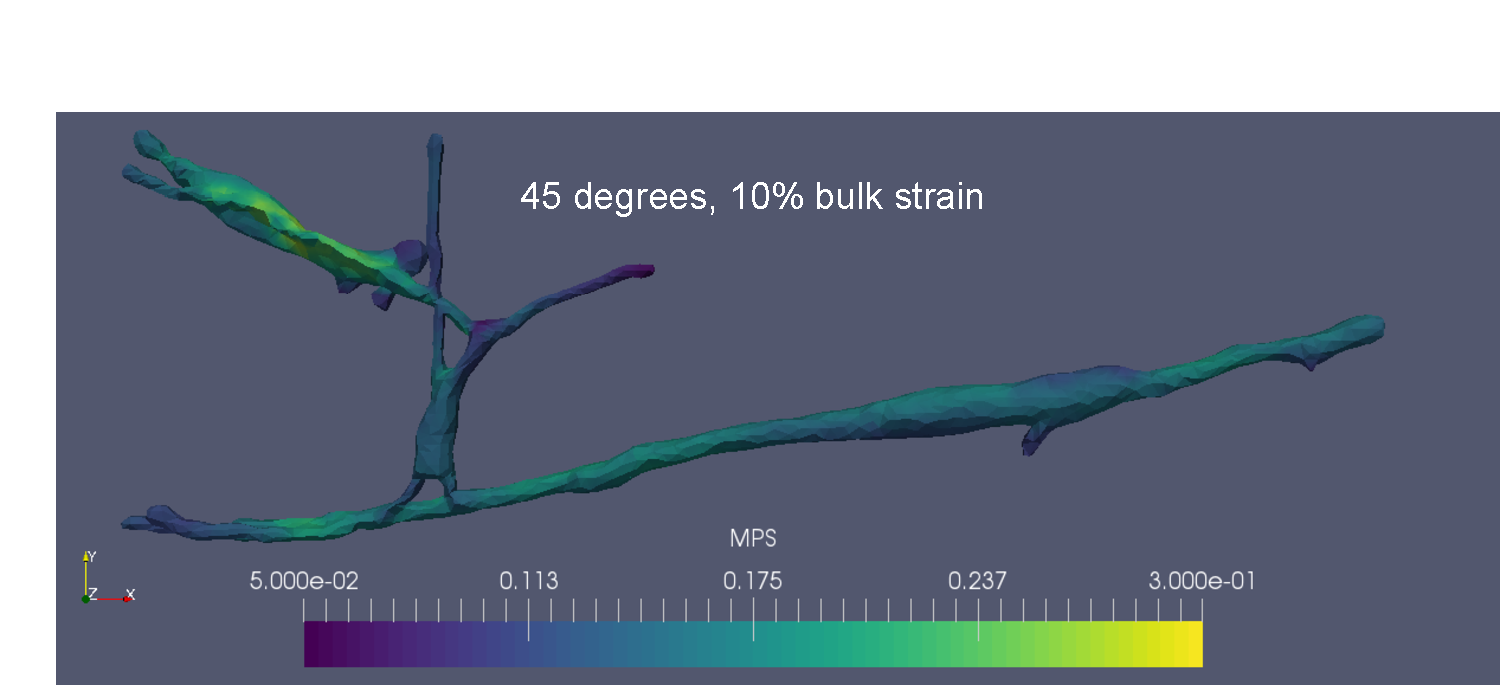
\includegraphics[height=3.5cm]{figure/MPS_rot45_strain10.pdf} &
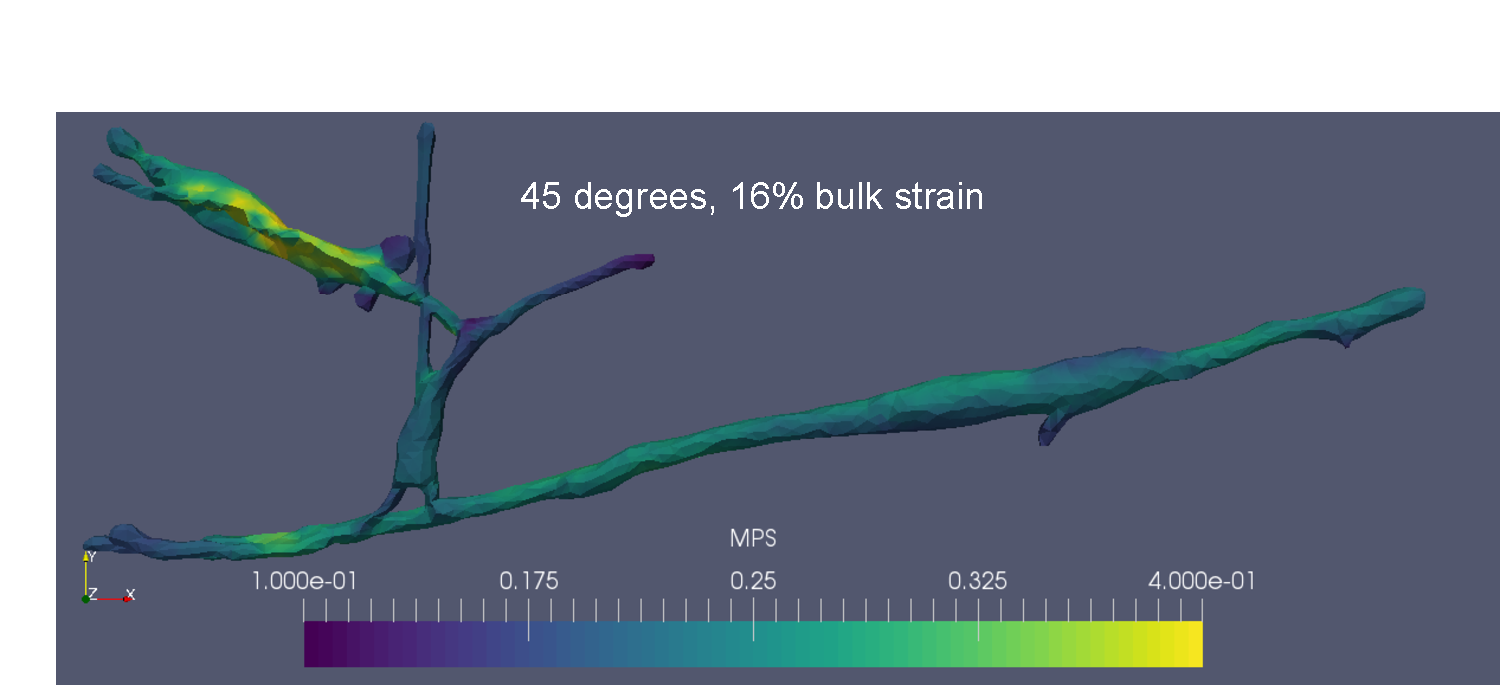
\includegraphics[height=3.5cm]{figure/MPS_rot45_strain16.pdf} \\
(a) & (b) \\
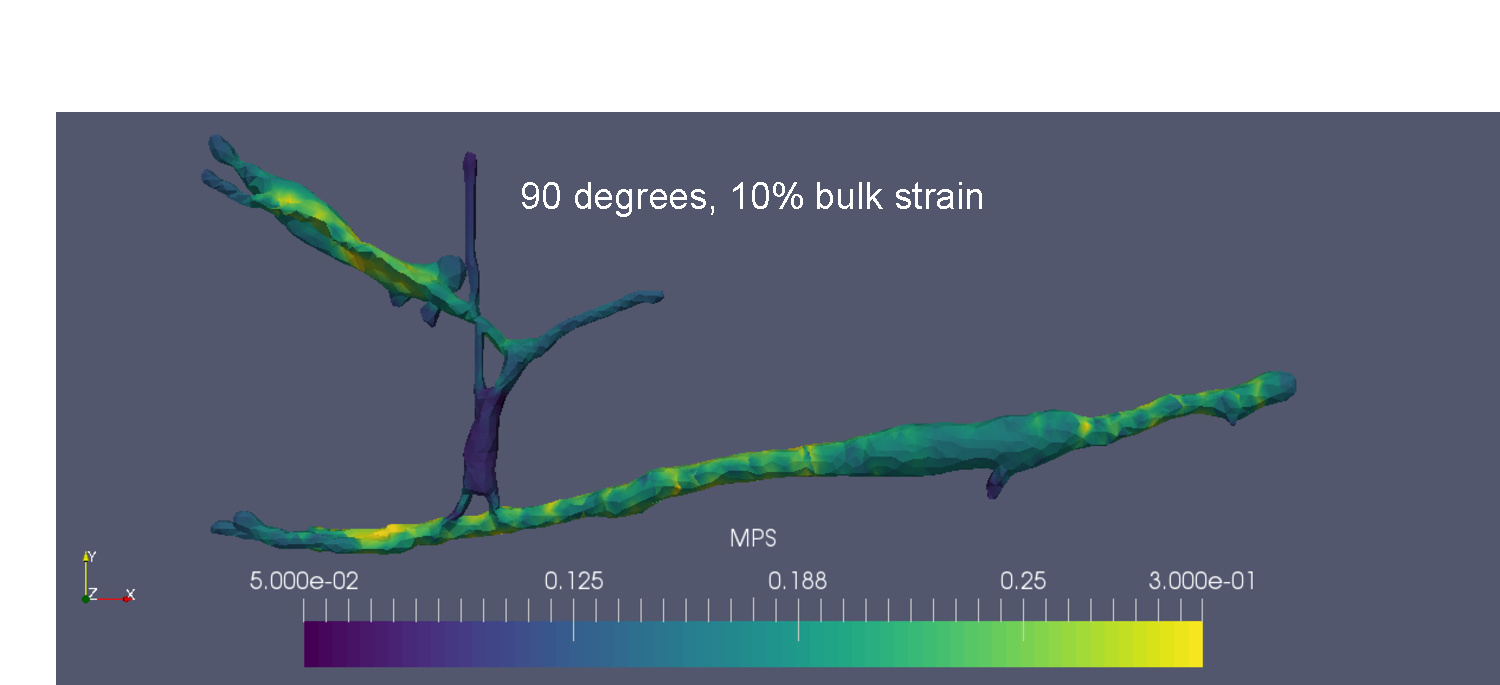
\includegraphics[height=3.5cm]{figure/MPS_rot90_strain10.pdf} & 
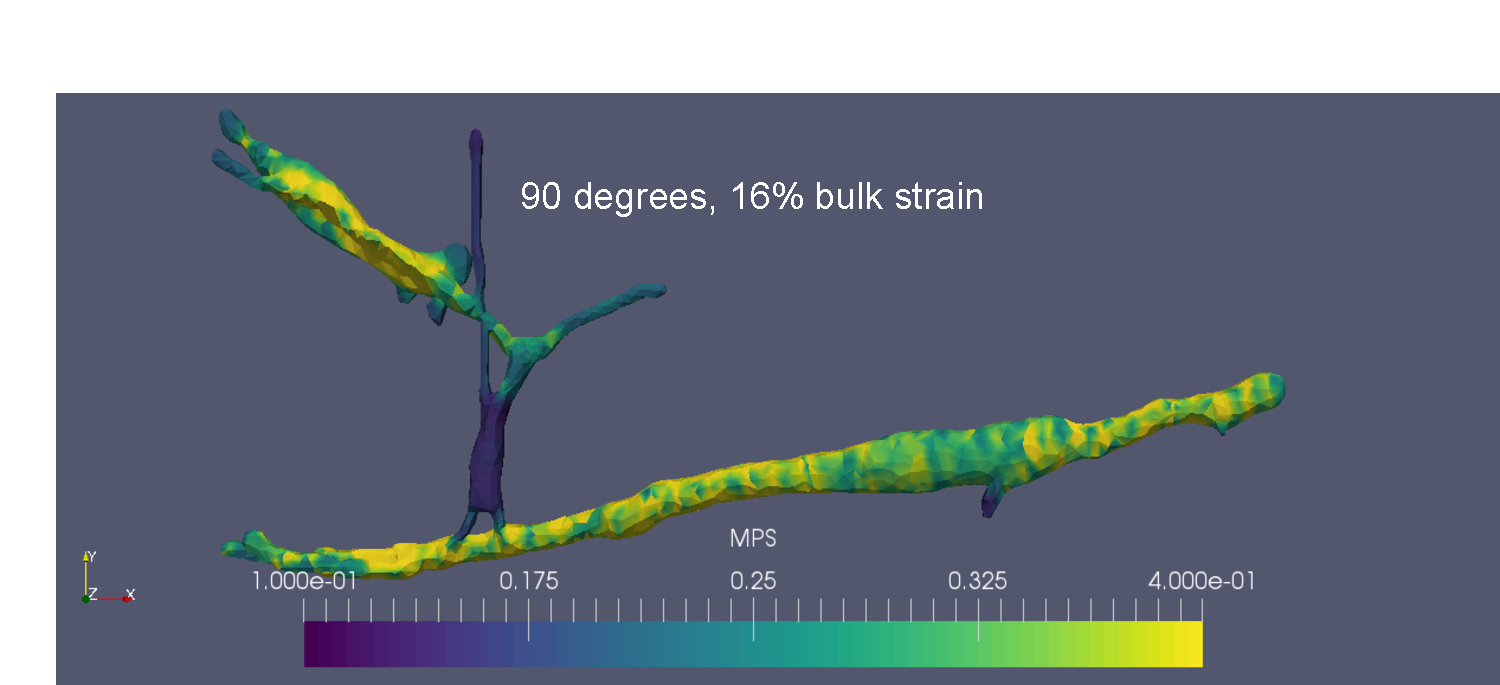
\includegraphics[height=3.5cm]{figure/MPS_rot90_strain16.pdf} \\
(c) & (d)
\end{array}
$
\end{center}
\caption{\label{fig:neuron_MPS} Color maps of maximum principal strain plotted on neuron structure for loading angles of 45 degrees (top row) and 90 degrees (bottom row). Bulk strains of 10$\%$ and 16$\%$ are considered. Note that the color bar ranges from 5$\%$ to 30$\%$ strain for bulk strain of 10$\%$ and from 10$\%$ to 40$\%$ for 16$\%$ bulk strain.}
\end{figure}
%

As seen in Fig.\ \ref{fig:neuron_MPS} and comparing to the 0 degree loading case in Fig.\ \ref{fig:neuron_0deg_MPS}, the strain distribution in the neuron varies significantly for different loading angles. In all scenarios, large portions of the neuron experience strains that are greater than the applied bulk strain in the collagen gel. The variation in strain distribution above can be quantitatively captured in ccdfs of the normalized MPS in the neuron, which are plotted in Fig.\ \ref{fig:neuron_ccdf_mps} for loading angles of 45 and 90 degrees at bulk strains of 10$\%$ and 16$\%$.
%
%45 degree distributions from N2P178/4-Neuron_FT_trcBC/MaxPrnStrn/PrincipalStrainDistr.m
%90 degree distribution from N2P178/3-Neuron_FT/MaxPrnStrn/PrincipalStrainDistr_FarField.m
\begin{figure}[ht]
\begin{center}
$
\begin{array}{cc}
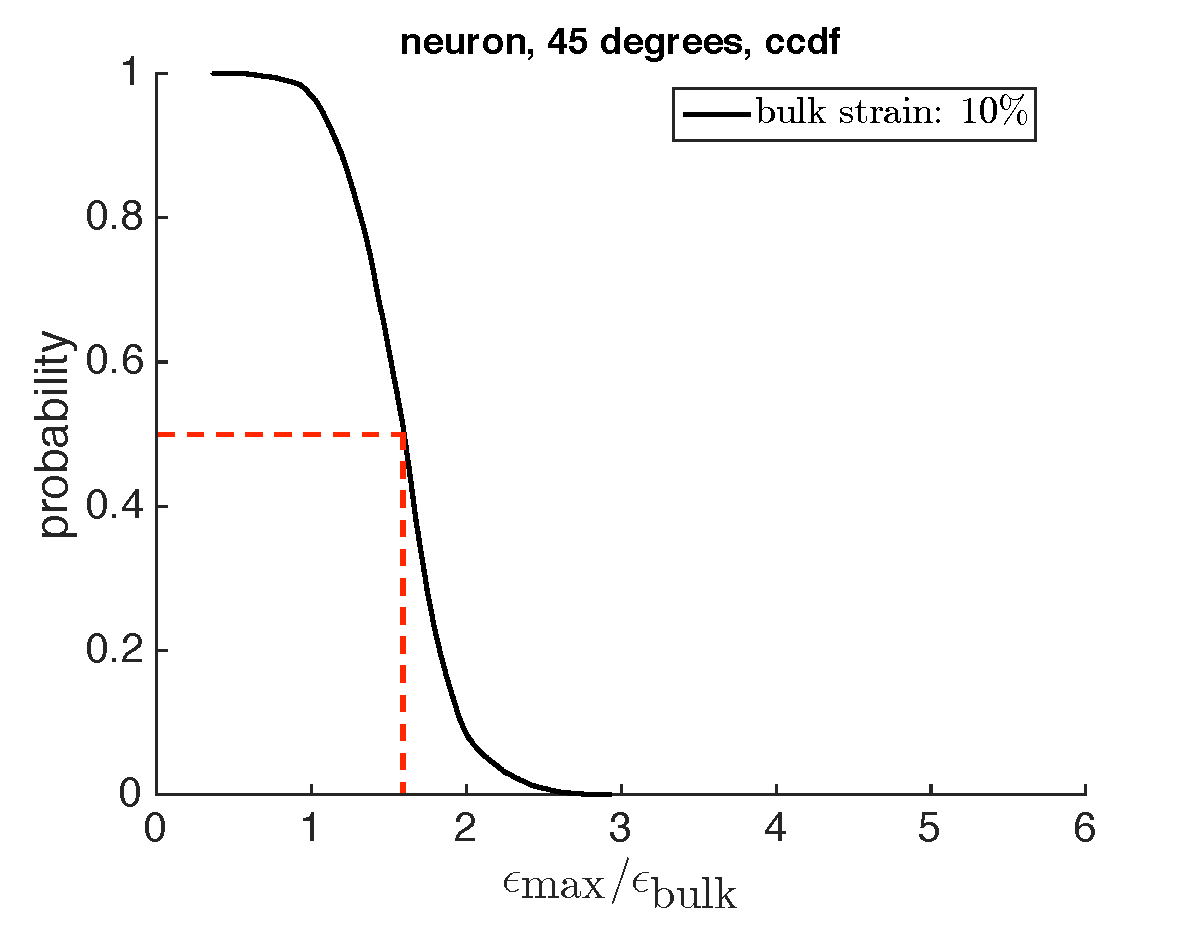
\includegraphics[height=6cm]{figure/neuron_45deg_MPS_ccdf_8.pdf} &
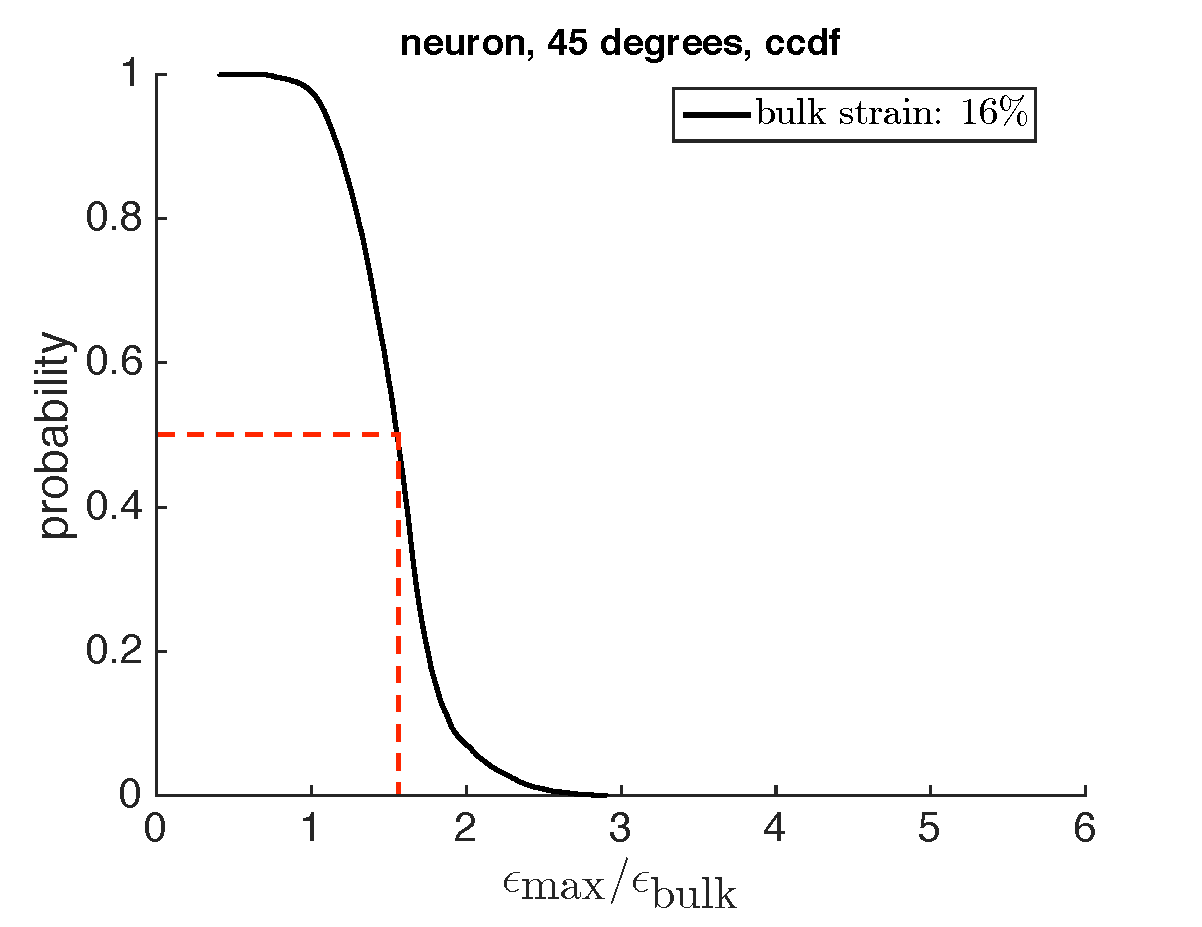
\includegraphics[height=6cm]{figure/neuron_45deg_MPS_ccdf_20.pdf} \\
(a) & (b) \\
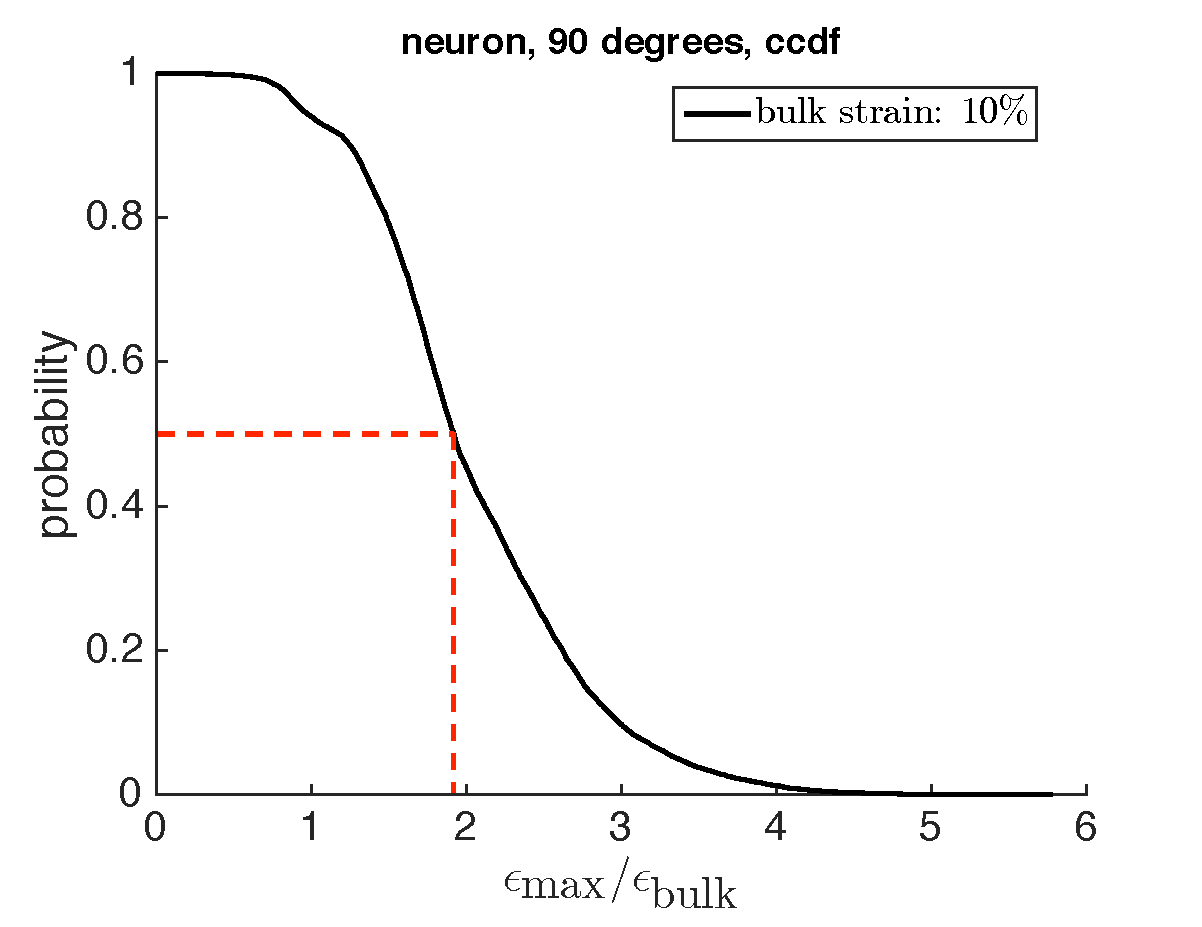
\includegraphics[height=6cm]{figure/neuron_90deg_MPS_ccdf_27.pdf} &
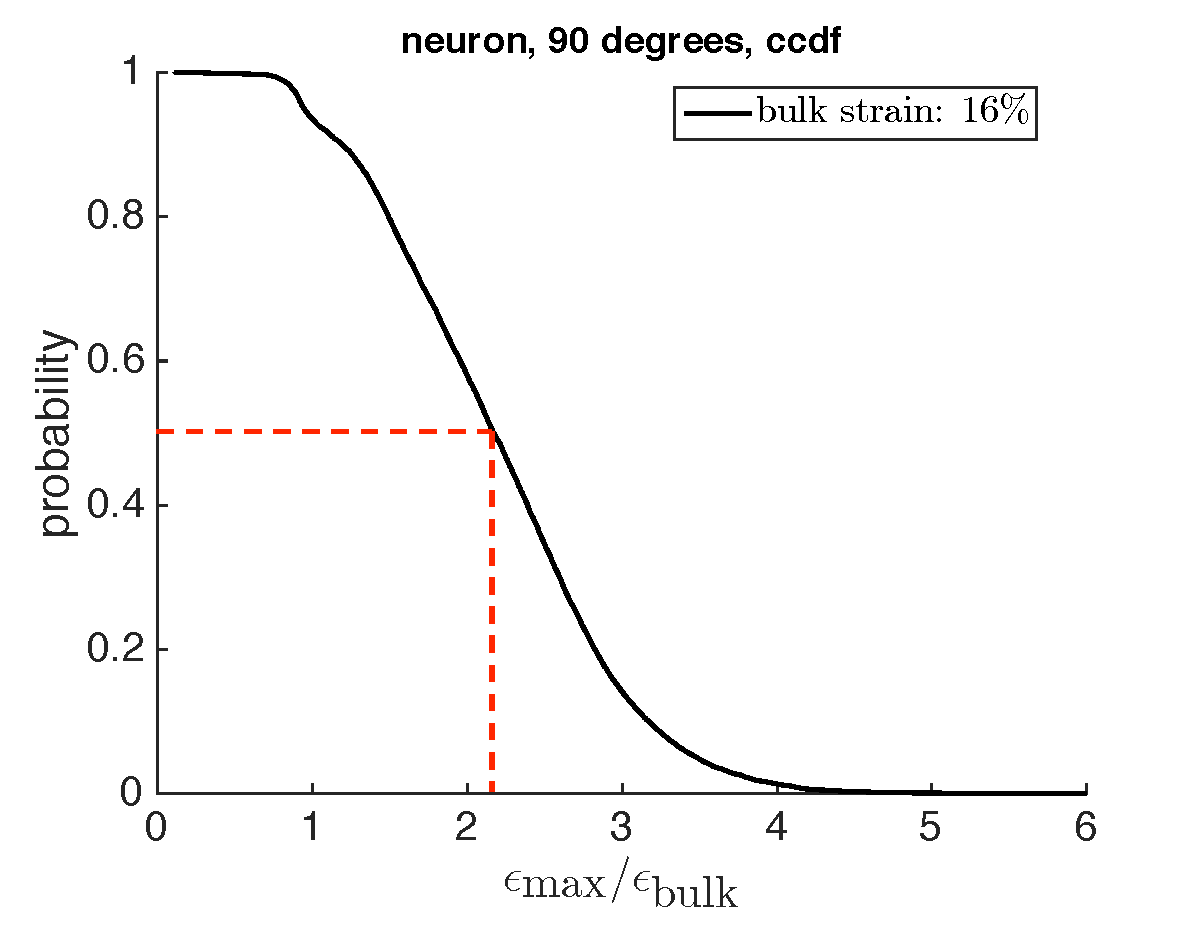
\includegraphics[height=6cm]{figure/neuron_90deg_MPS_ccdf_47.pdf} \\
(c) & (d) 
\end{array}
$
\end{center}
\caption{\label{fig:neuron_ccdf_mps} ccdfs of normalized MPS in the neuron for loading angles of 45 (top row) and 90 (bottom row) degrees. Bulk strains of 10$\%$ and 16$\%$ in the collagen gel are considered. The averages (50$\%$ probability) are indicated by the dashed red lines. } 
\end{figure}
%

Consistent with what is observed in the strain distribution when comparing the color maps of Figs.\ \ref{fig:neuron_0deg_MPS} and \ref{fig:neuron_MPS}, the ccdfs vary significantly for different loading directions. For both non painful and painful ligament loading, the average normalized MPS for 45 and 90 degree loading is greater than that of the 0 degree loading case (Fig.\ \ref{fig:neuron_ccdf_0deg_mps}). Although the average strain amplification in the neuron is greater when loaded at 45 degrees than when loaded at 0 degrees, the tail of the ccdf for the 45 degree case is shorter with a maximum strain amplification that is less than 3 times. In the 90 degree loading case, the average strain amplification is approximately double the applied bulk strain and the tail of the ccdf reaches to nearly 6 times that of the applied bulk strain. 

Physiologically, the 90 degree loading configuration will give rise to the most damage in the neuron structure when the surrounding collagen is loaded. As seen in color maps of MPS in Fig.\ \ref{fig:neuron_MPS}, large portions of the neuron are deformed perpendicular to its axial direction for the 90 degree loading case. The anisotropic mechanical behavior of the neuron coupled with a surrounding gel structure that becomes stiffer with deformation leads to the large amplification of strain when the neuron is loaded in transversely.




%Variation in the shape and spread of the neuron strain distributions at different bulk strains is greatest in the case of 90 degree loading, where the spread of the distributions increase with larger bulk strain. In contrast, the variations in shape and spread of the neuron strain distributions are small for the 0 and 45 degree loading cases. Additional insight can be gained by separating the neuron strain distribution into contributions from the cell bodies and axons. The distributions of maximum principal strain in the cell bodies and axons are plotted in Fig.\ \ref{fig:rgns_ccdf_mps}.
%%
%\begin{figure}[ht]
%\begin{center}
%$
%\begin{array}{ccc}
%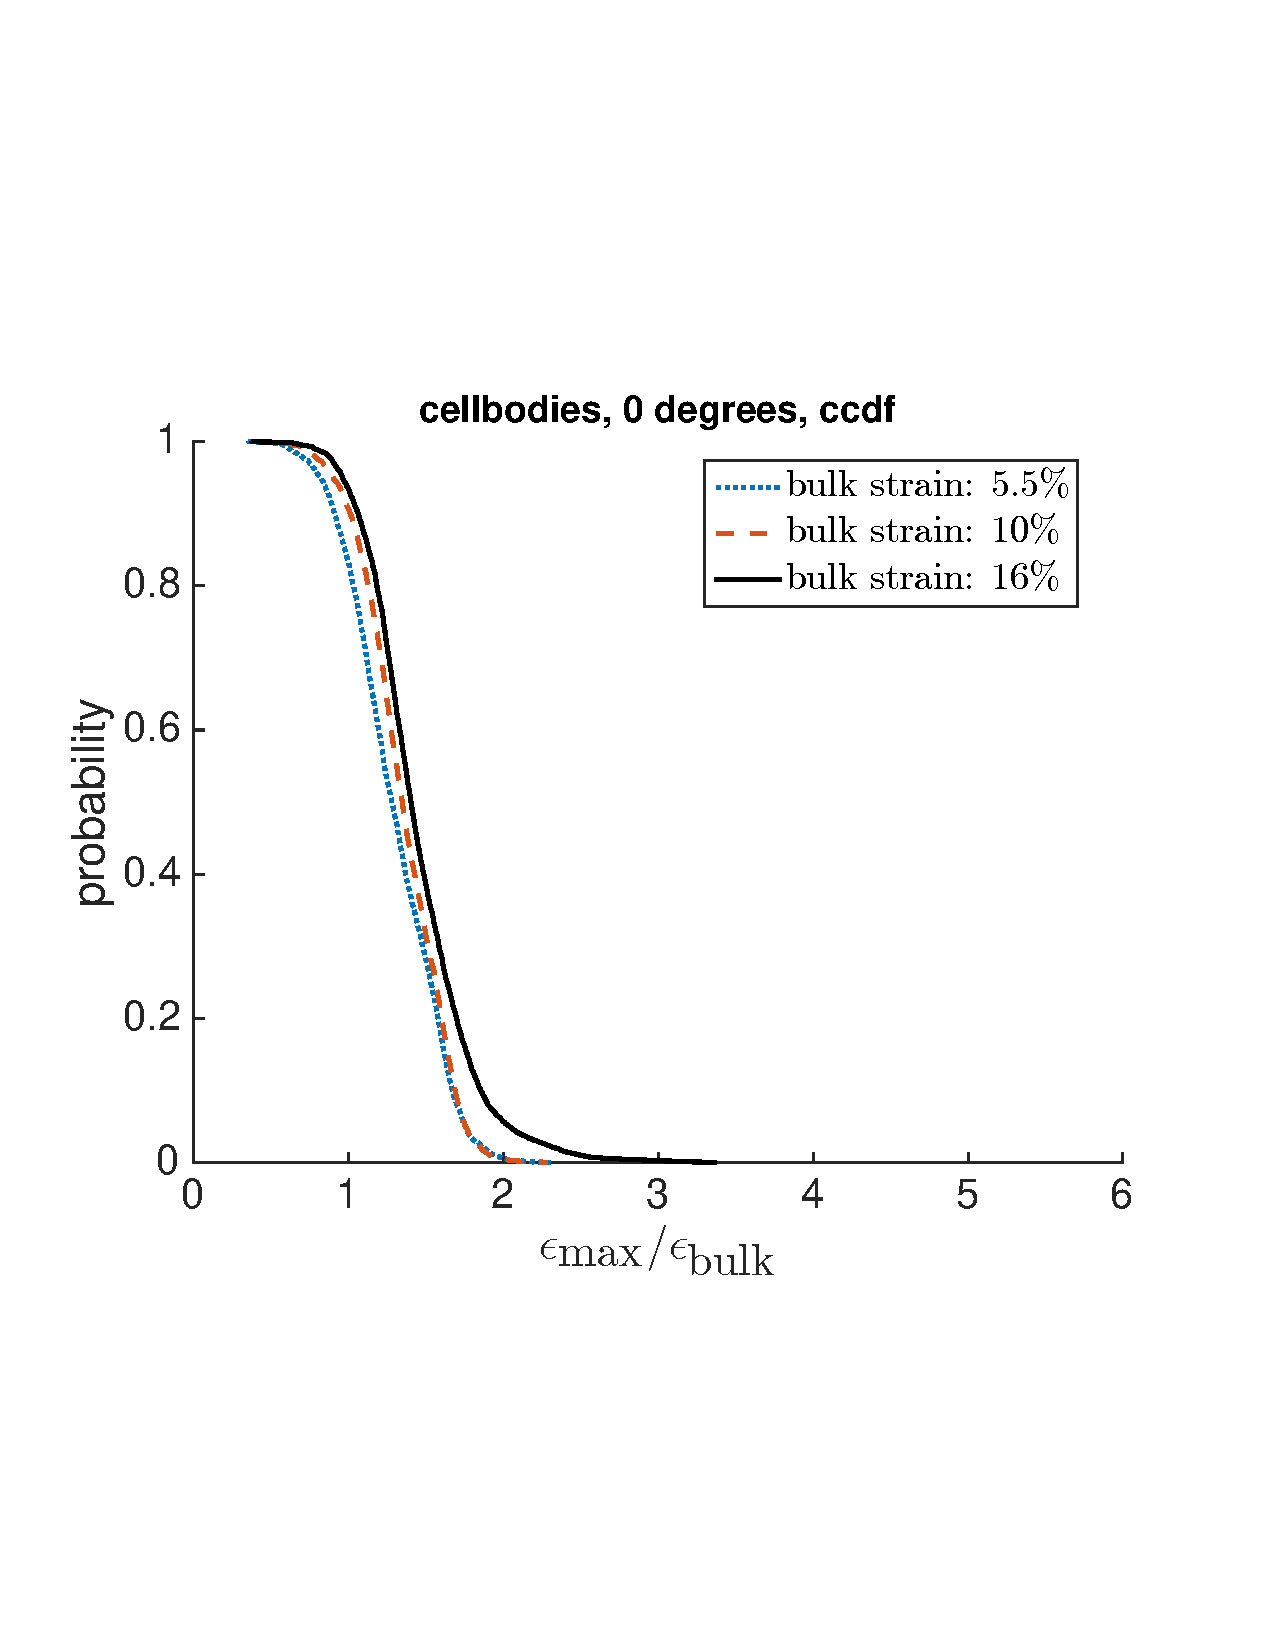
\includegraphics[height=4.5cm]{figure/rot0_FT50_128_1920_ccdf_cellbodies_compare_stps.pdf} & 
%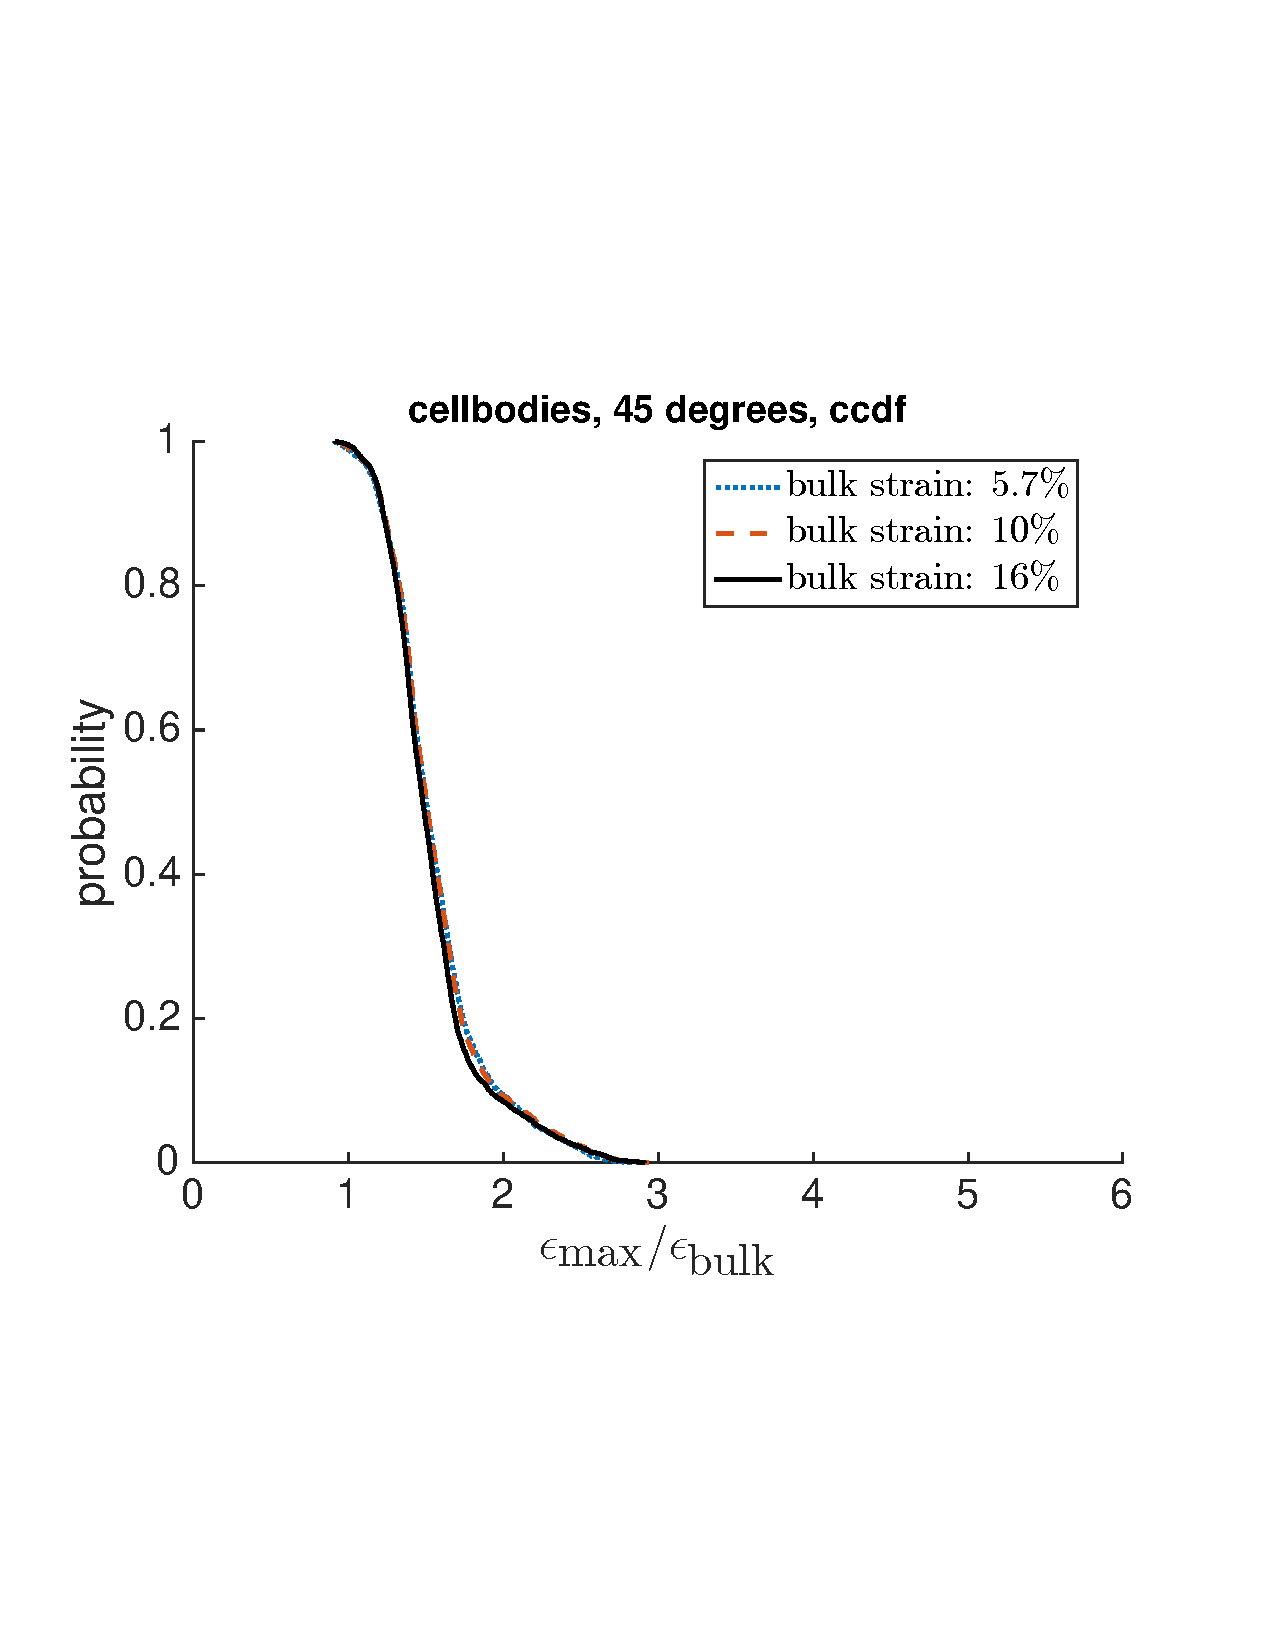
\includegraphics[height=4.5cm]{figure/rot45_FT50_128_1920_ccdf_cellbodies_compare_stps.pdf} & 
%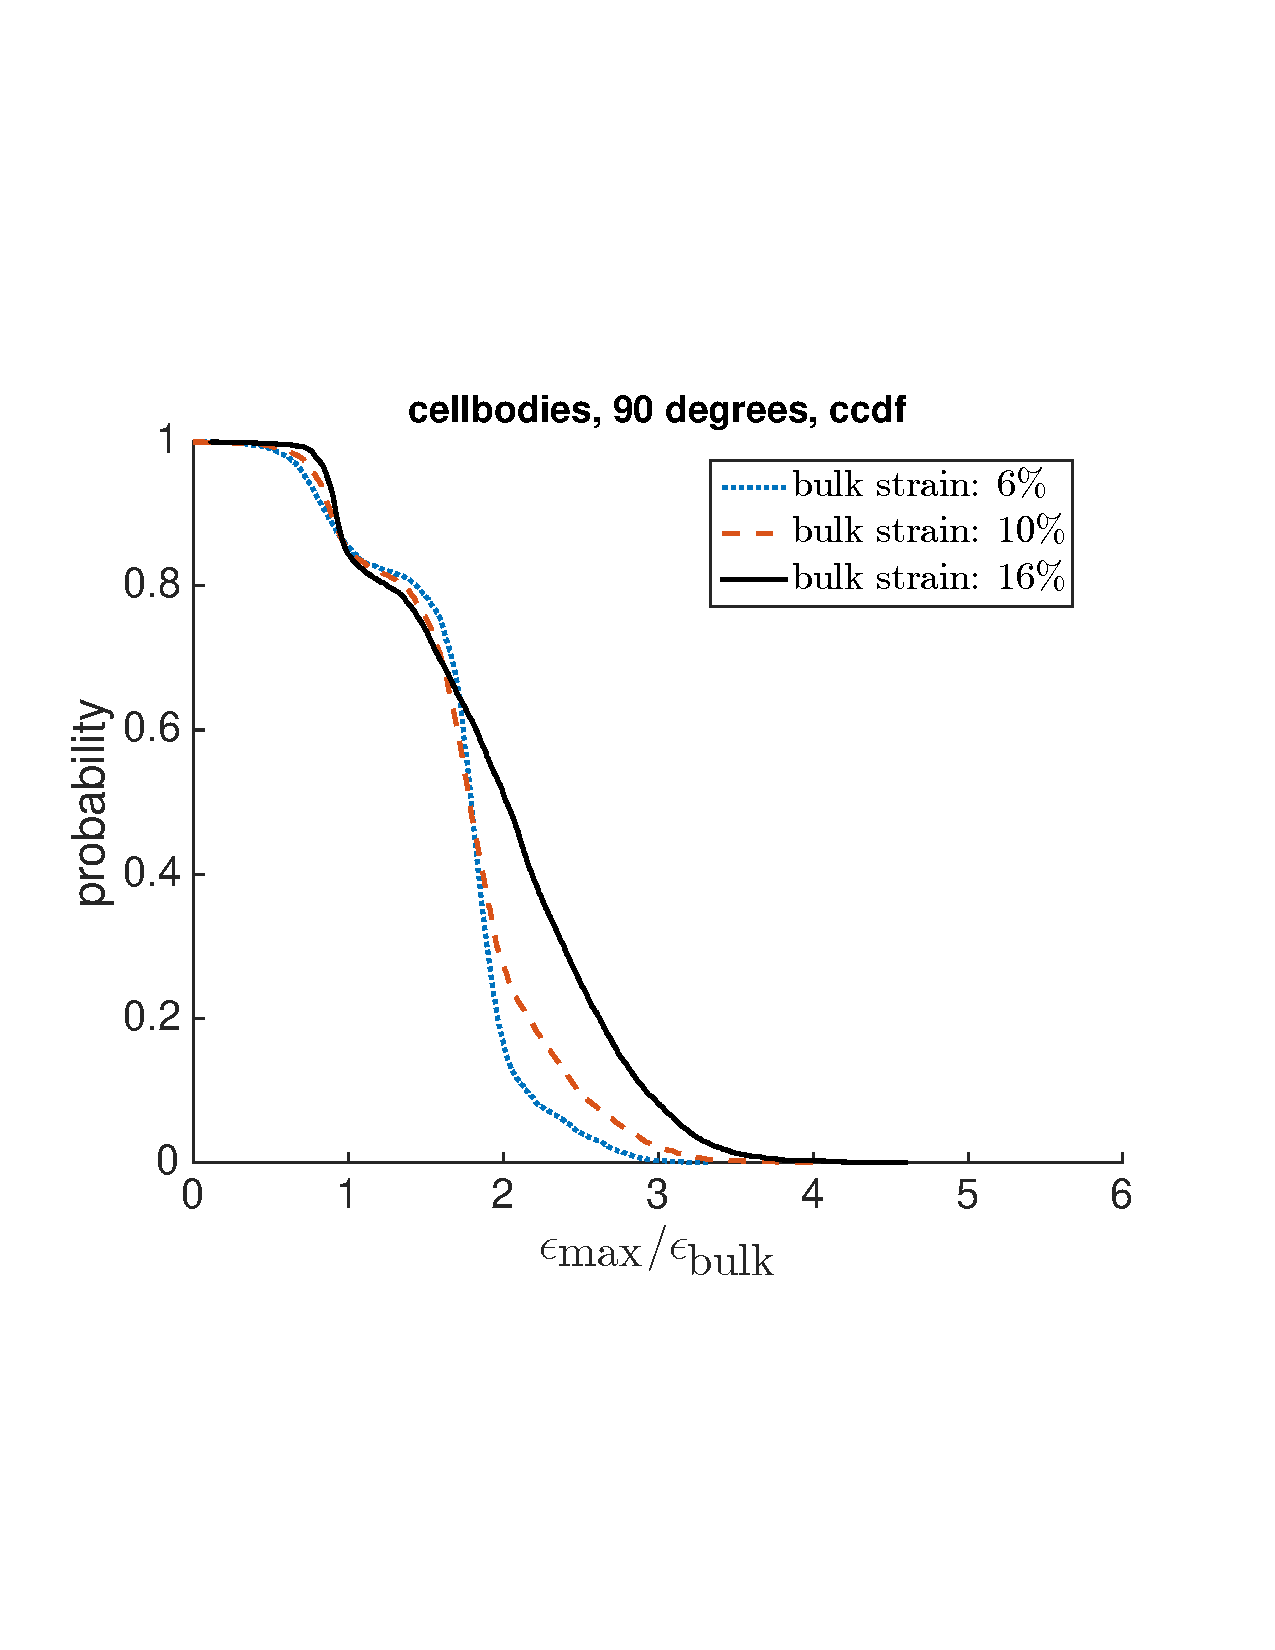
\includegraphics[height=4.5cm]{figure/rot90_FT_dspBC50_a30_128_1920_ccdf_cellbodies_compare_stps_farfield.pdf} \\
%(a) & (b) & (c) \\
%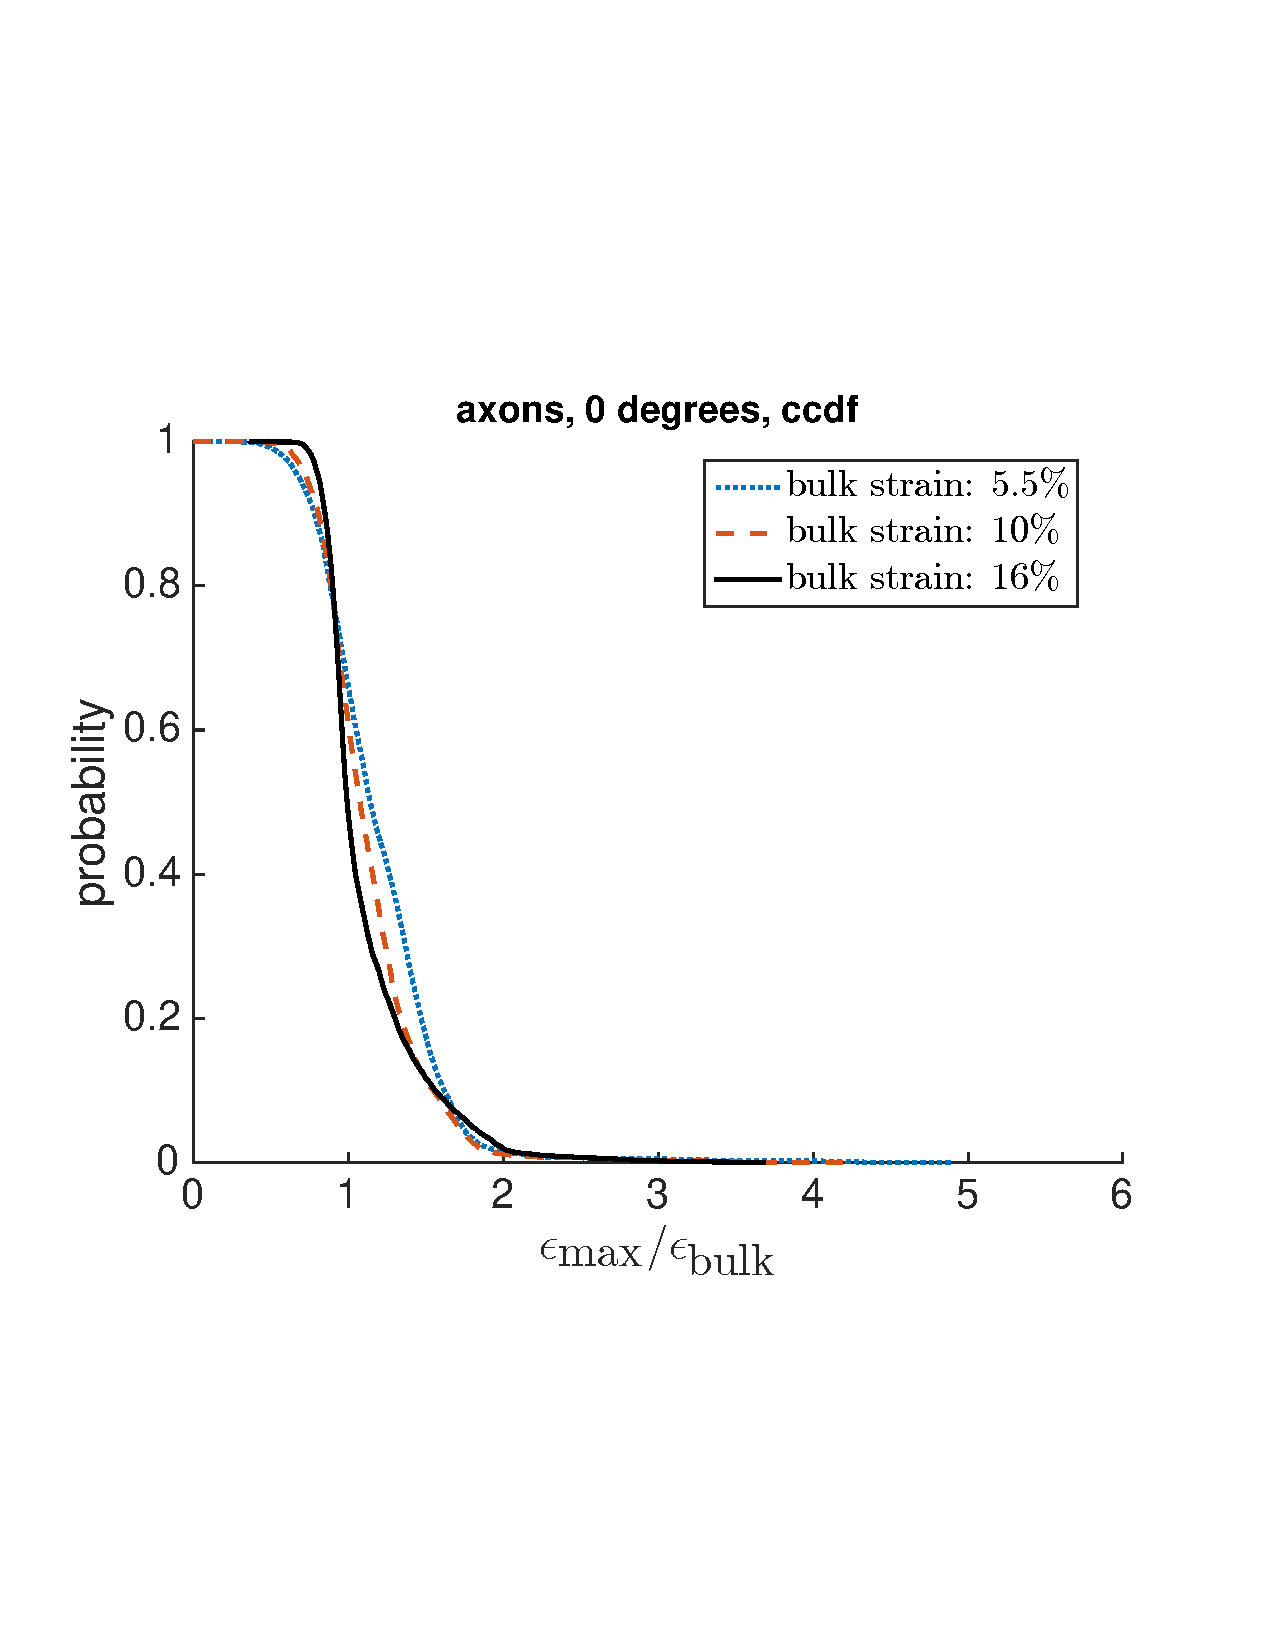
\includegraphics[height=4.5cm]{figure/rot0_FT50_128_1920_ccdf_axons_compare_stps.pdf} &
%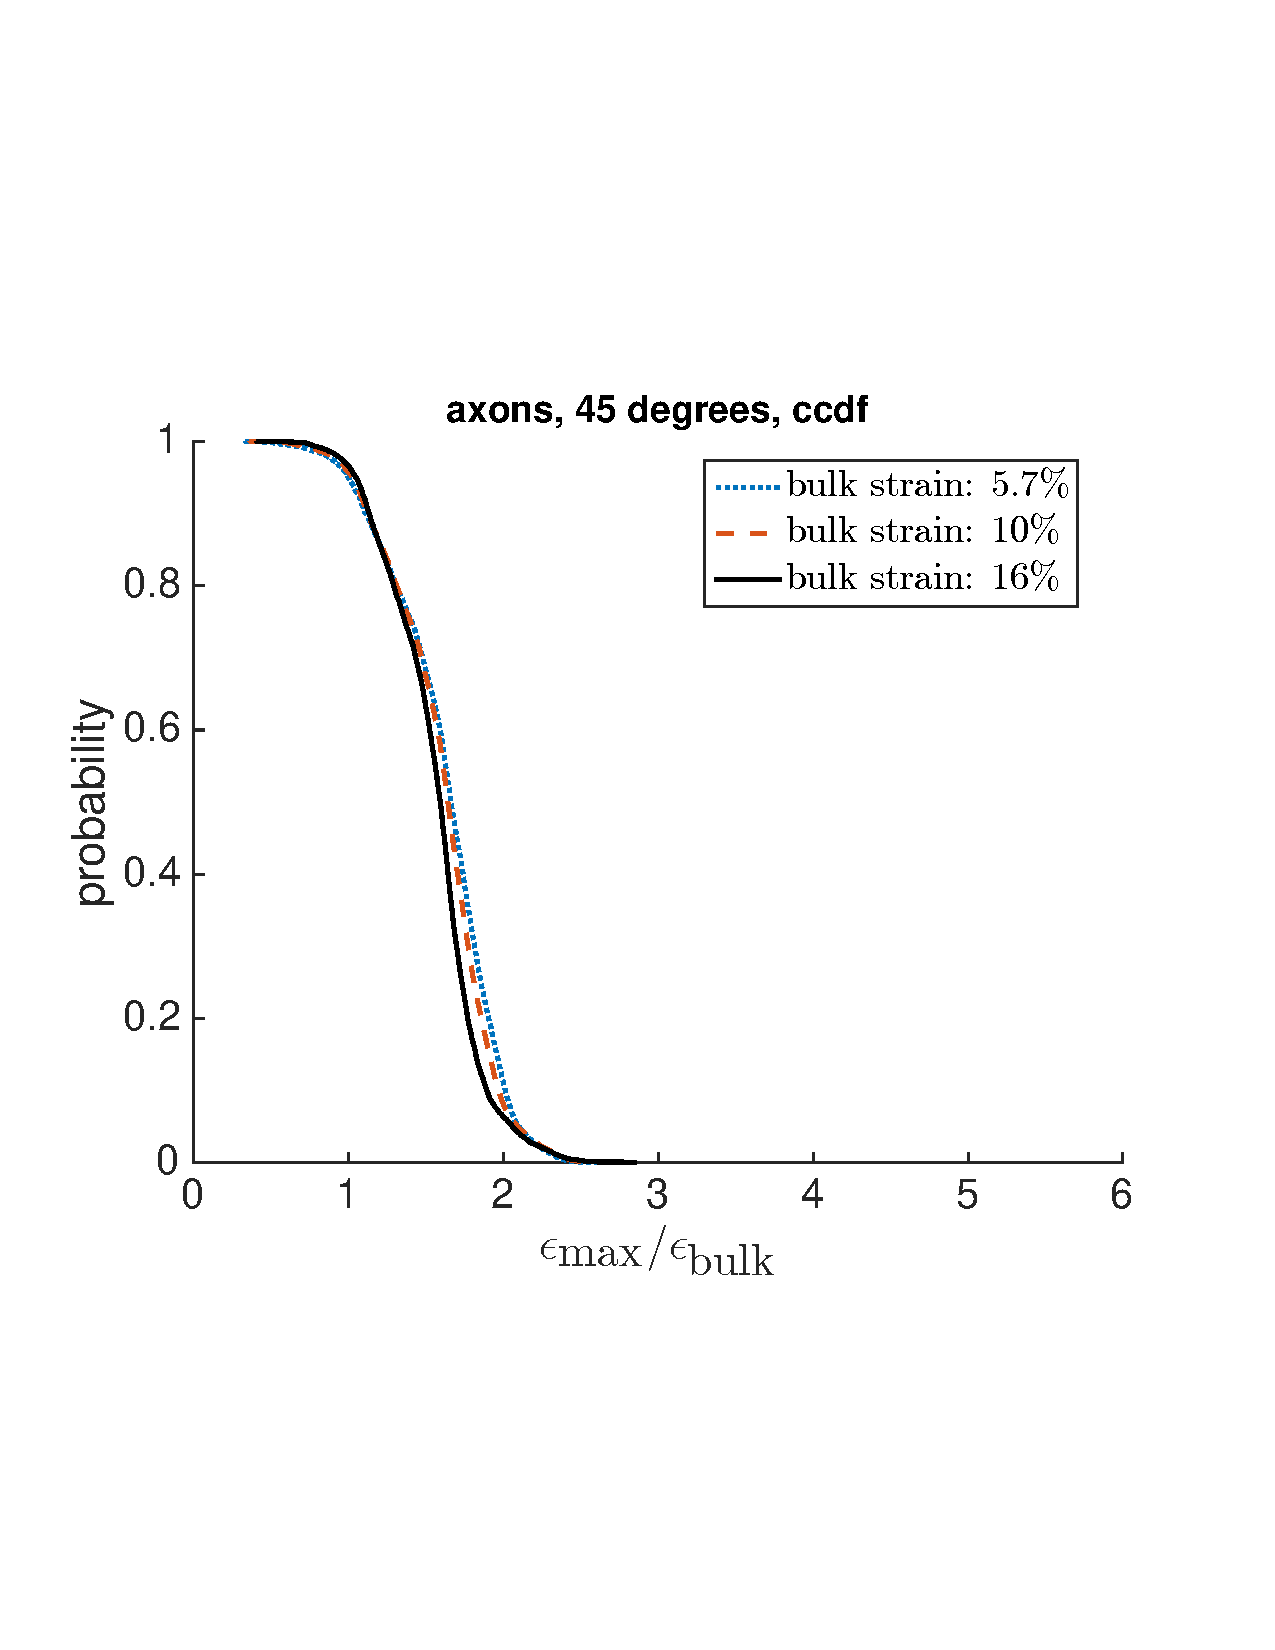
\includegraphics[height=4.5cm]{figure/rot45_FT50_128_1920_ccdf_axons_compare_stps.pdf} &
%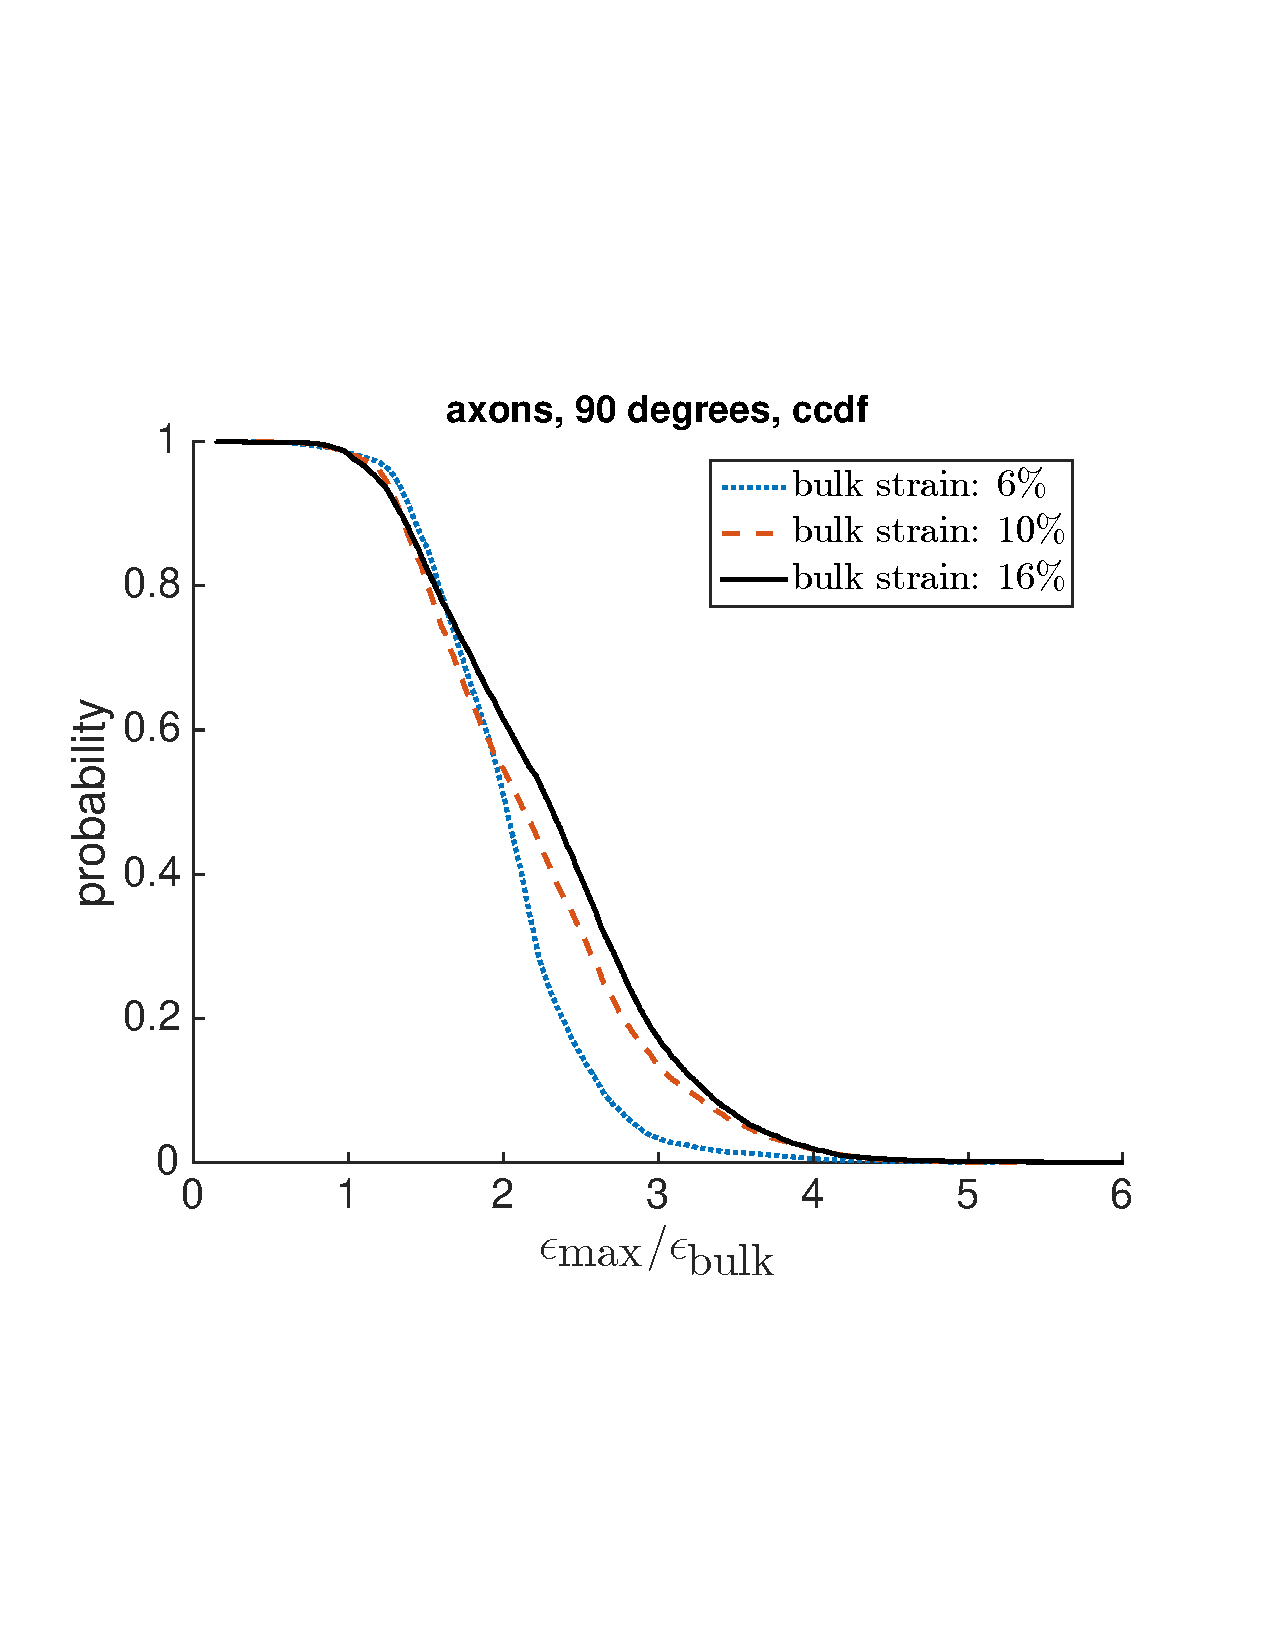
\includegraphics[height=4.5cm]{figure/rot90_FT_dspBC50_a30_128_1920_ccdf_axons_compare_stps_farfield.pdf} \\
%(d) & (e) & (f)
%\end{array}
%$
%\end{center}
%\caption{\label{fig:rgns_ccdf_mps} Distributions of maximum principal strain (ccdf) in the cell bodies (top row) and axons (bottom row) for loading angles of (a,d) 0 degrees, (b,e) 45 degrees, and (c,f) 90 degrees. For each loading angle, distributions for bulk strains of 5 - 6 $\%$ (dotted blue line), 10$\%$ (dashed red line), and 16$\%$ (solid black line) are plotted. The values of $\epsilon_{\text{max}}$ are normalized by the bulk strain, $\epsilon_{\text{bulk}}$.  }
%\end{figure}
%%
%
%The separate distributions for the cell bodies and axons provide additional details about the variations in shape and spread of the neuron distributions in Fig.\ \ref{fig:neuron_ccdf_mps}. For the 0 degree loading case, variations in the distribution at different bulk strains become more apparent. For the cell bodies, the distribution shifts to the right for larger bulk strains indicating that the amplification in the local strain becomes larger with more deformation in the surrounding gel. On the contrary, the middle portion of the axon distribution shifts to the left with increasing bulk strains indicating that the local strain amplification decreases with more deformation in the surrounding gel. The response in the cell bodies and axons cancel out resulting in only slight variations in the overall neuron strain distribution. 
%
%For the 45 degree loading case, variations only arise in the axon distribution. Therefore, the variations seen in the overall neuron distribution is solely due to variations in the axon. Similar to the 0 degree loading case, the axon distribution for the 45 degree loading shifts to the left with larger bulk strains indicating a decrease in the local strain amplification as the surrounding gel is increasingly deformed.
%
%For the 90 degree loading case, large variations are seen in both the cell body and axon distributions. For the cell bodies, the subtle step feature seen in the overall neuron distribution becomes more apparent. This step feature corresponds to two regimes of strain which are clearly seen in the over plot of maximum principal strain on the neuron in Figs.\ \ref{fig:neuron_MPS}(e) and (f). For both the cell body and axon, the distributions shift to the right with increasing bulk strains indicating that the local strain amplification increases with increasing deformation in the surrounding gel. 
%
%The results above indicate that the local strains experienced by the neuron is significantly larger than the applied load on the surrounding gel. The extent of local strain amplification depends on the configuration of the neuron relative to the loading angle. To clarify the cause of local strain amplification in the neuron, the axial strains along a region of the neuron structure are examined.
%
%%=========================================================================================================
%\subsection{Axial Strain Distributions}
%In this section we examine the axial strains, which are more directly linked to the actual geometry of the neuron structure, to shed light on the relationship between local strain amplification and the relative configuration of the neuron with respect to loading angle. Our analysis focuses on a portion of the neuron structure that lies along a single axis. This portion of the neuron is highlighted in Fig.\ \ref{fig:axial_schematic} where the axes on which the strain distributions are calculated are also specified (i.e., axis 1 and axis 2). 
%%
%\begin{figure}[ht]
%\begin{center}
%$
%\begin{array}{c}
%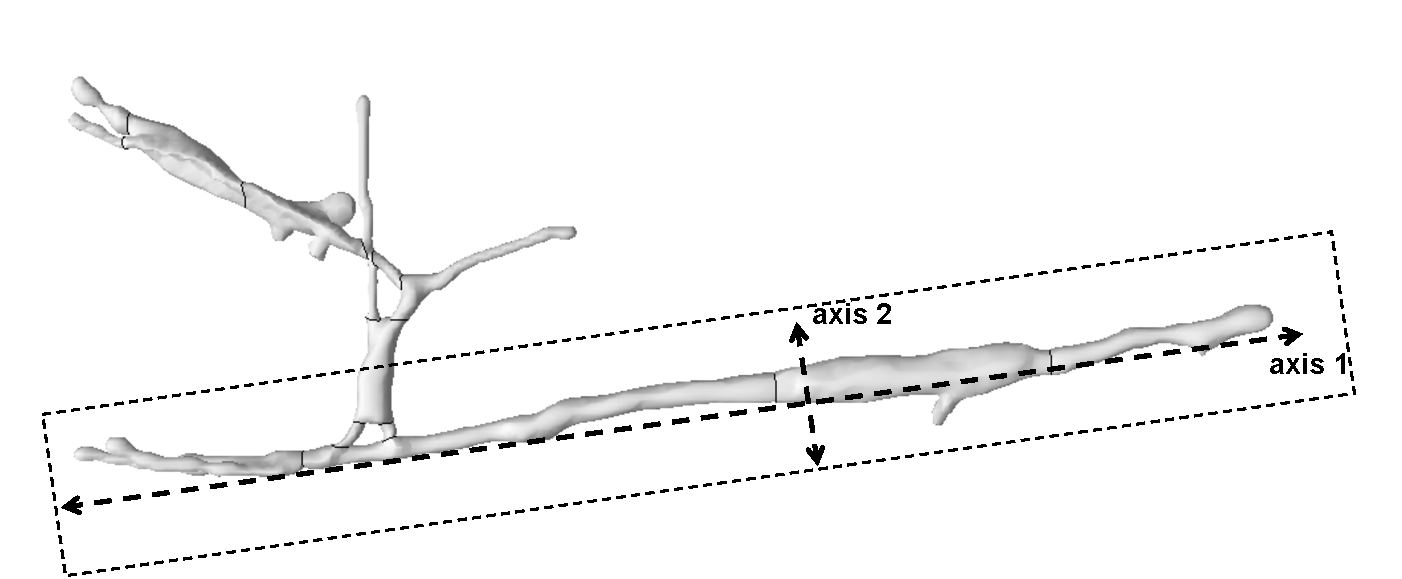
\includegraphics[height=4cm]{figure/axial_coords_schematic.pdf} 
%\end{array}
%$
%\end{center}
%\caption{\label{fig:axial_schematic} Schematic showing the region (rectangular box) and the axes (dashed lines) that are examined.}
%\end{figure}
%%
%
%Distributions of the axial strains along axes 1 and 2 are plotted in Fig.\ \ref{fig:axial_distr} for different loading angles. Depending on the loading angle, axes 1 and 2 will experience either tensile or compressive axial strains. In the case of tensile strains, the ccdf in Eq.\ \eqref{eq:ccdf} is used, while the cdf in Eq.\ \eqref{eq:cdf} is applied for compressive strains. For the 0 degree loading case the axial strains along axis 1 are tensile while those along axis 2 are compressive. The opposite is true for the 90 degree loading case - compressive strain in axis 1 and tensile strain in axis 2 - because the load direction is orthogonal. In the case of 45 degree loading, axis 1 experiences tensile strains while axis 2 experiences mostly compressive strains with a small fraction of the structure experiencing tensile strains.
%%
%% images from N2P178/5-Neuron_LocalAxon_Strain/MaxPrnStrn/PrincipalStranDistr.m
%\begin{figure}[ht]
%\begin{center}
%$
%\begin{array}{ccc}
%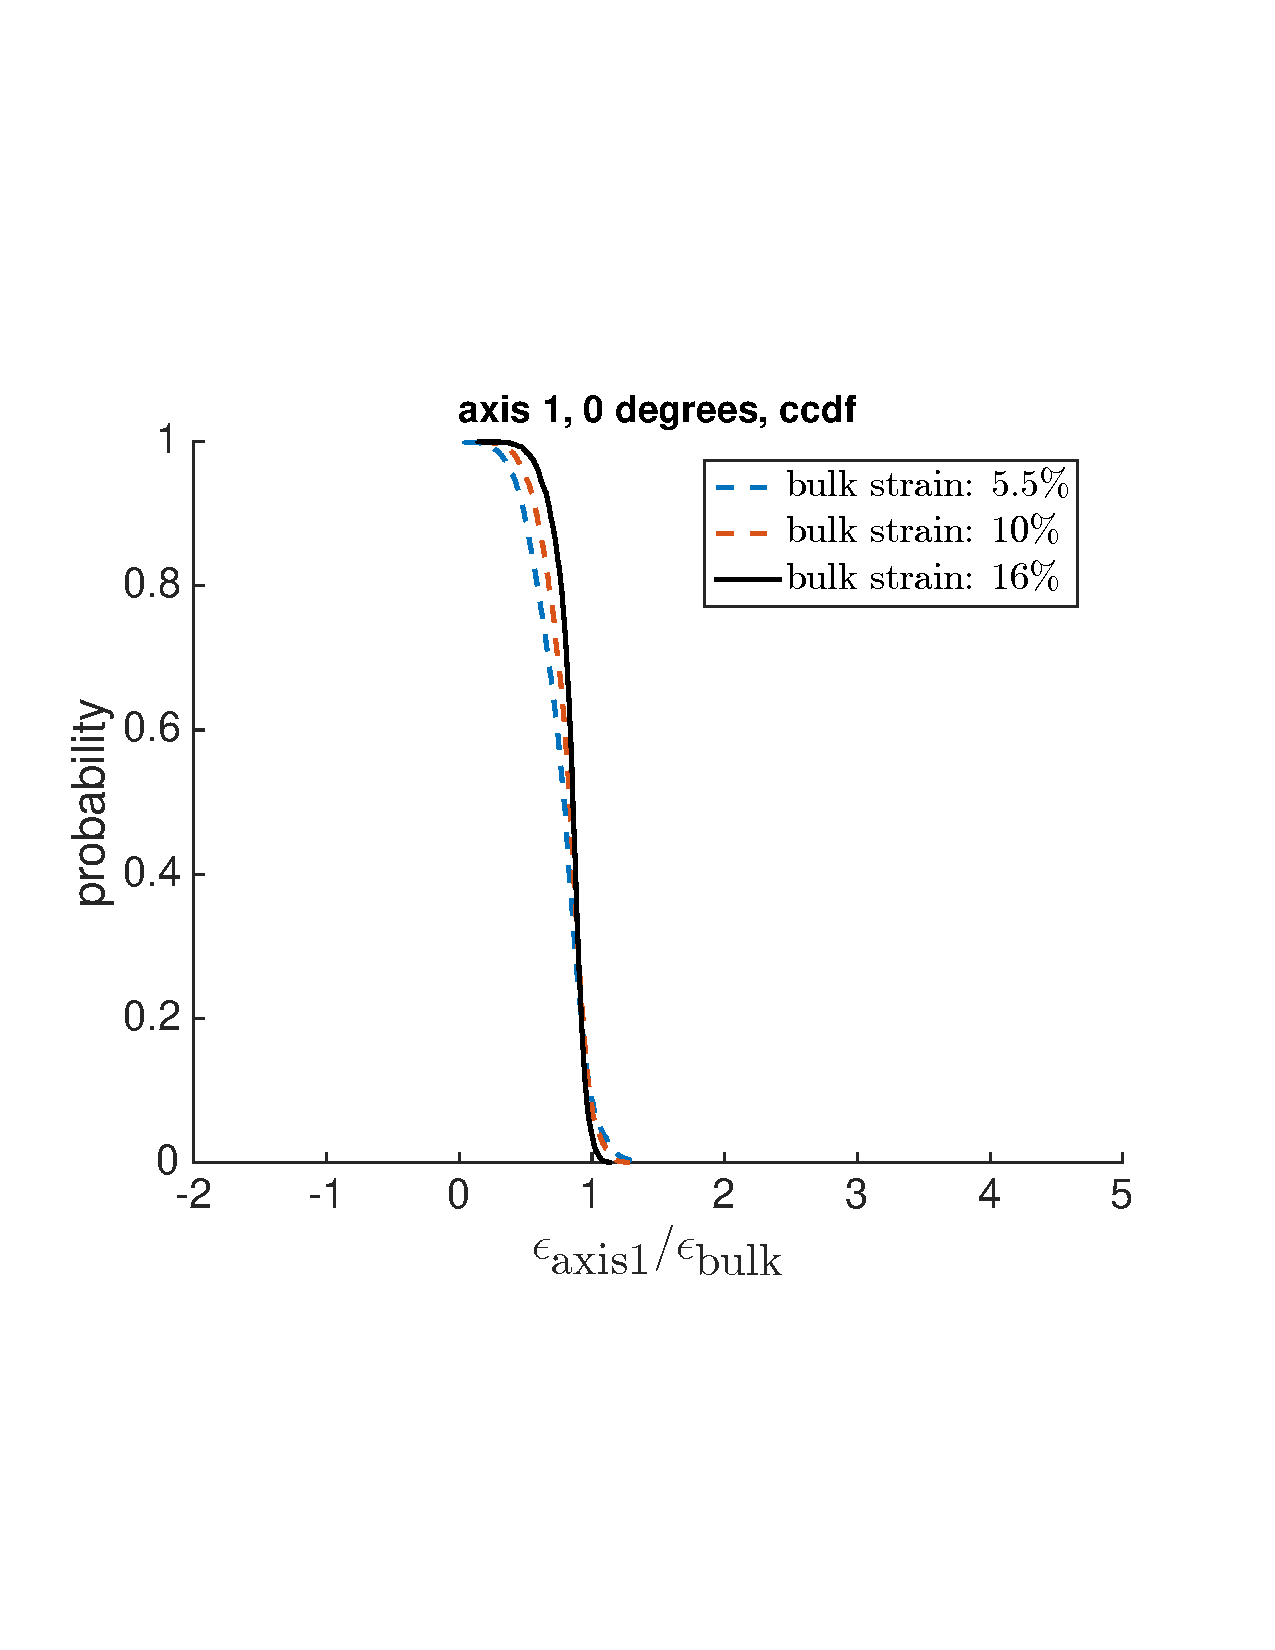
\includegraphics[height=4.5cm]{figure/rot0_FT50_strn11_128_1920_axial_ccdf_axis1_compare_stps.pdf} & 
%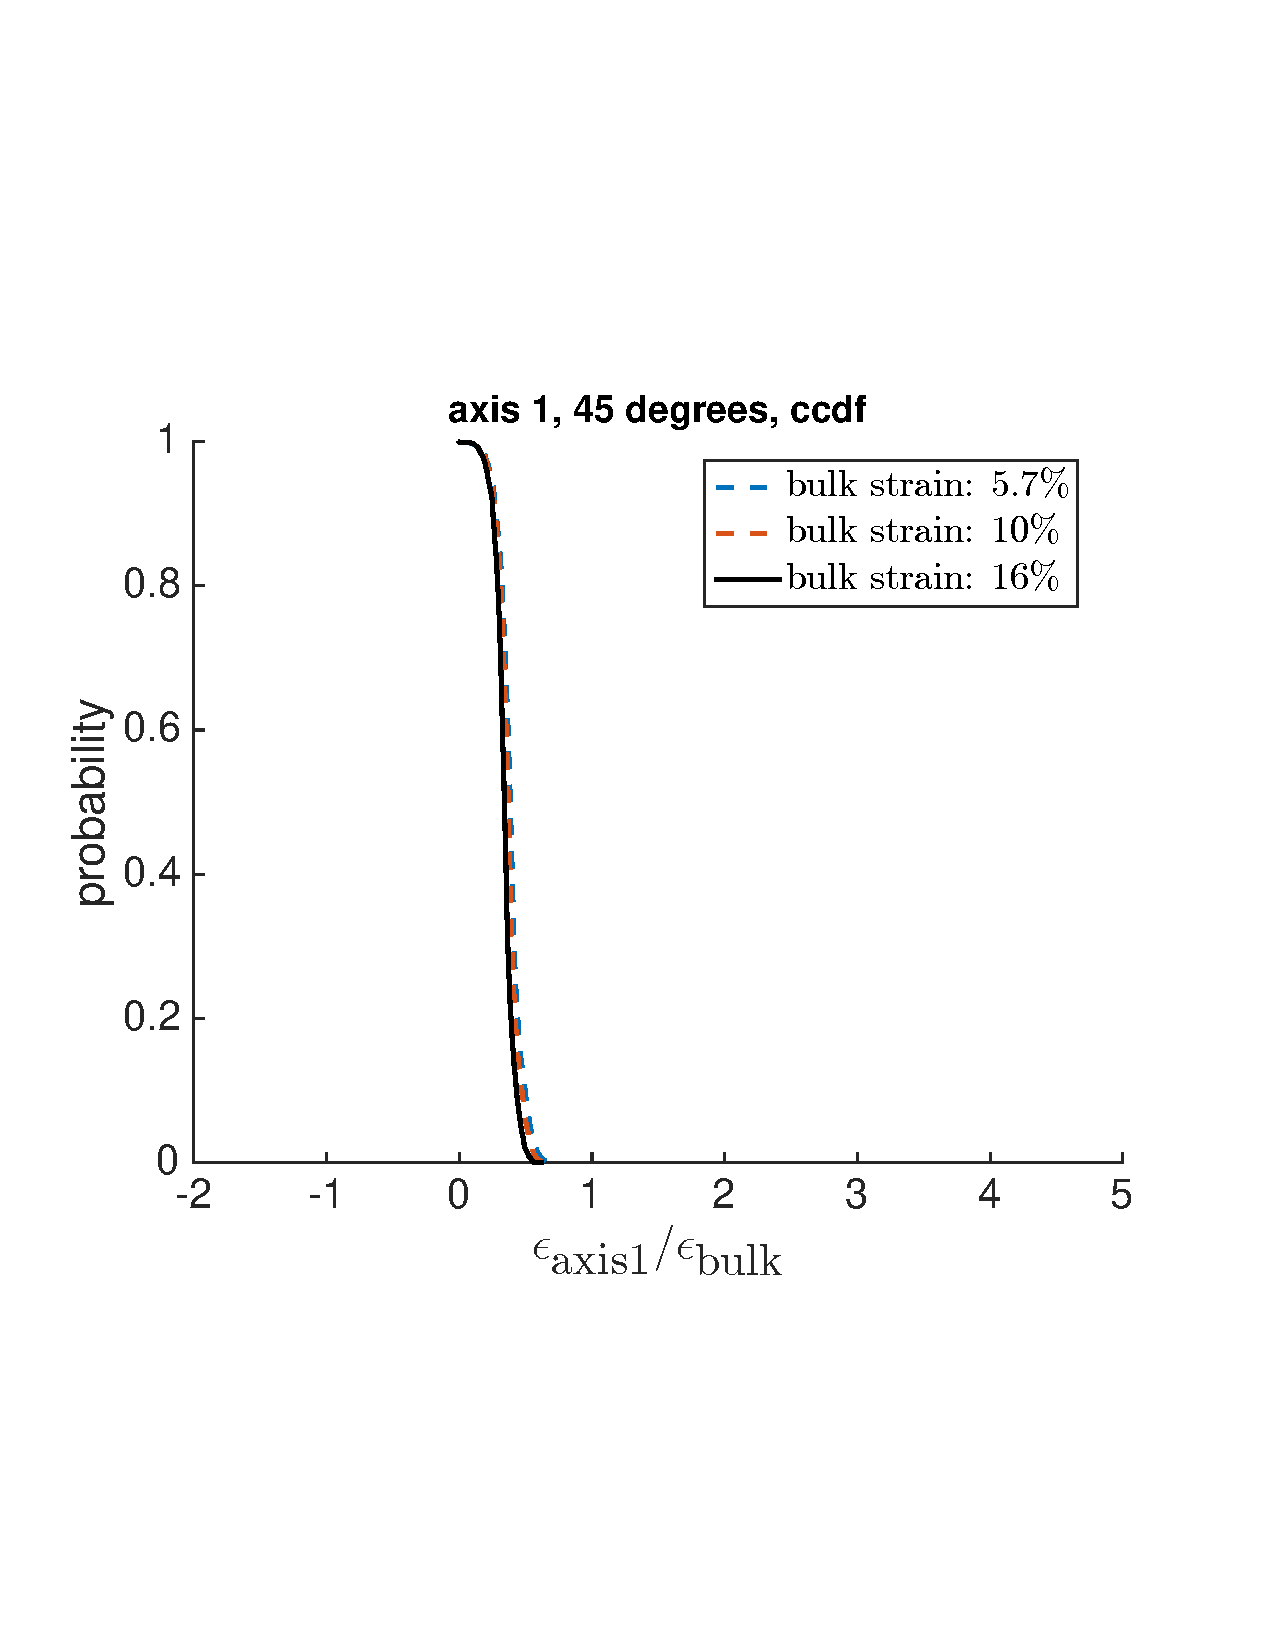
\includegraphics[height=4.5cm]{figure/rot45_FT50_strn11_128_1920_axial_ccdf_axis1_compare_stps.pdf} &
%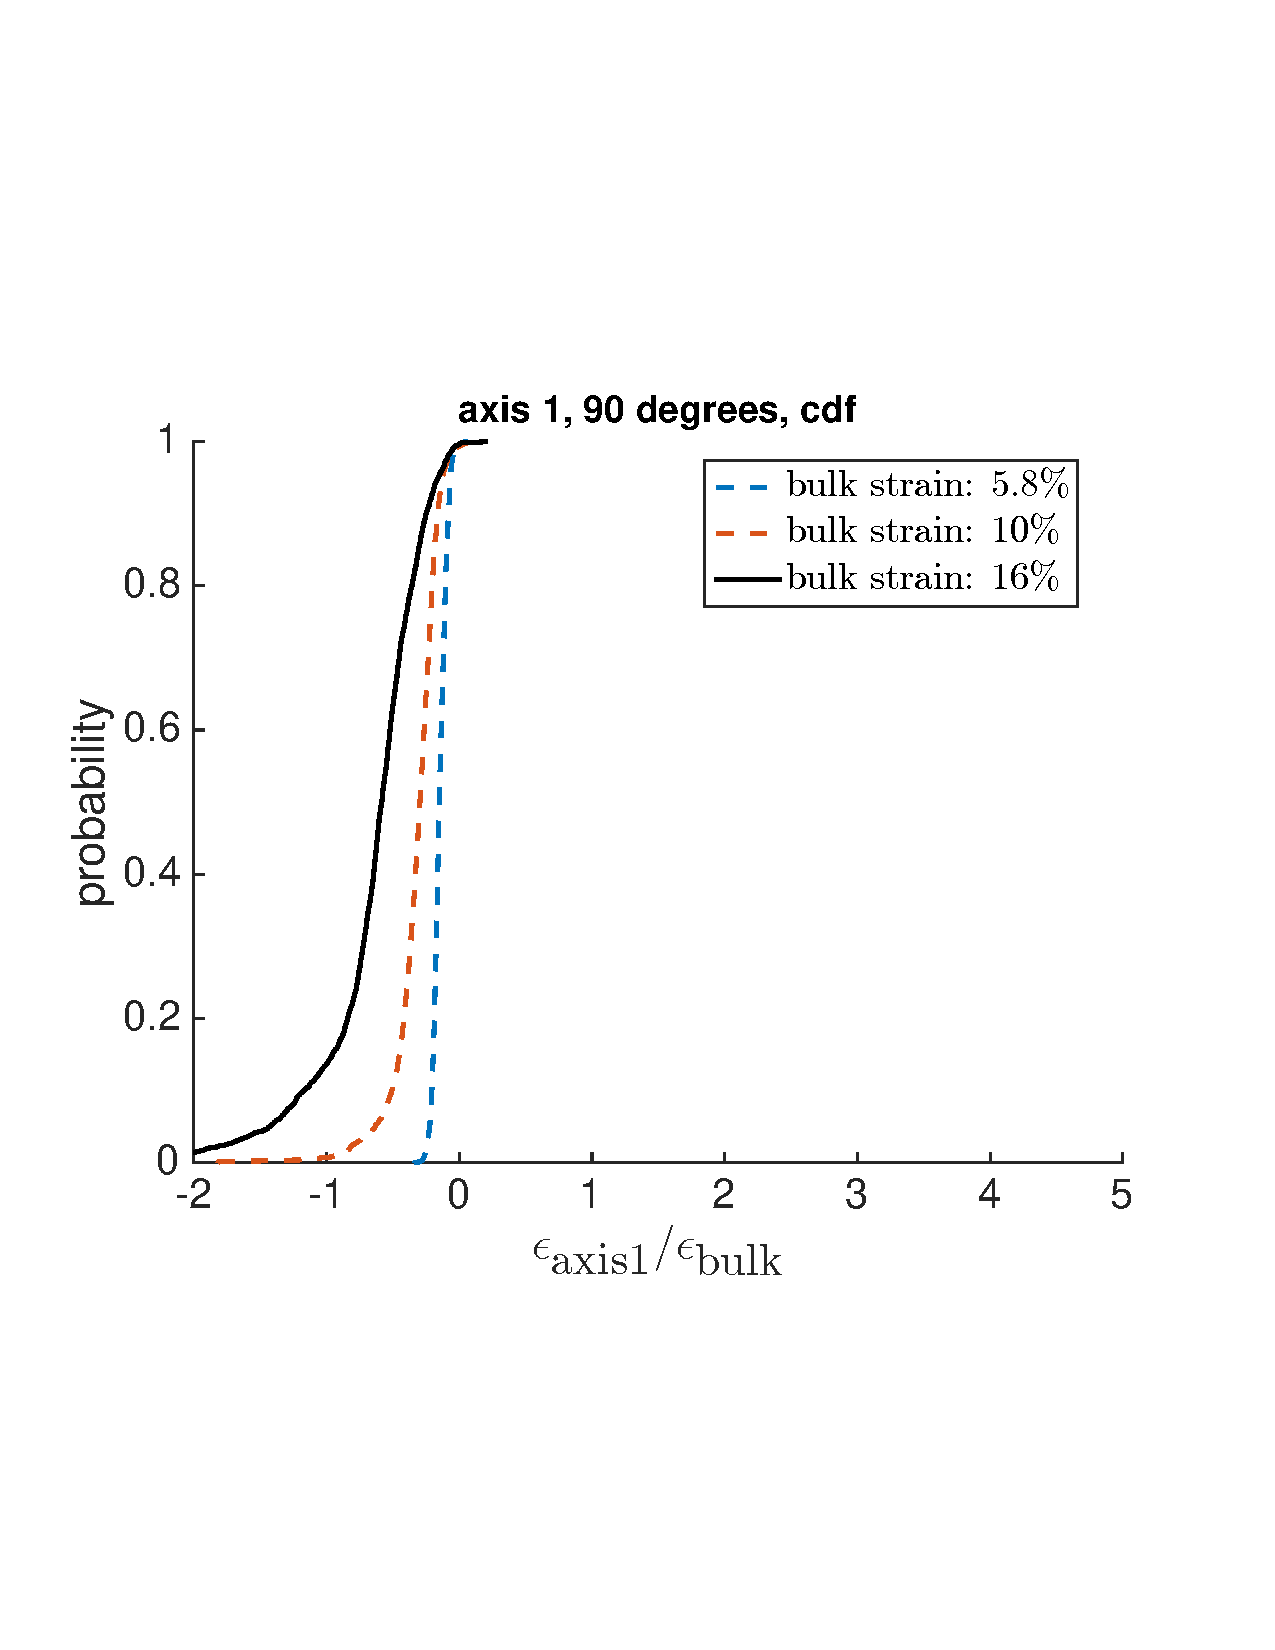
\includegraphics[height=4.5cm]{figure/rot90_FT50_strn11_128_1920_axial_cdf_axis1_compare_stps.pdf} \\
%(a) & (b) & (c) \\ 
%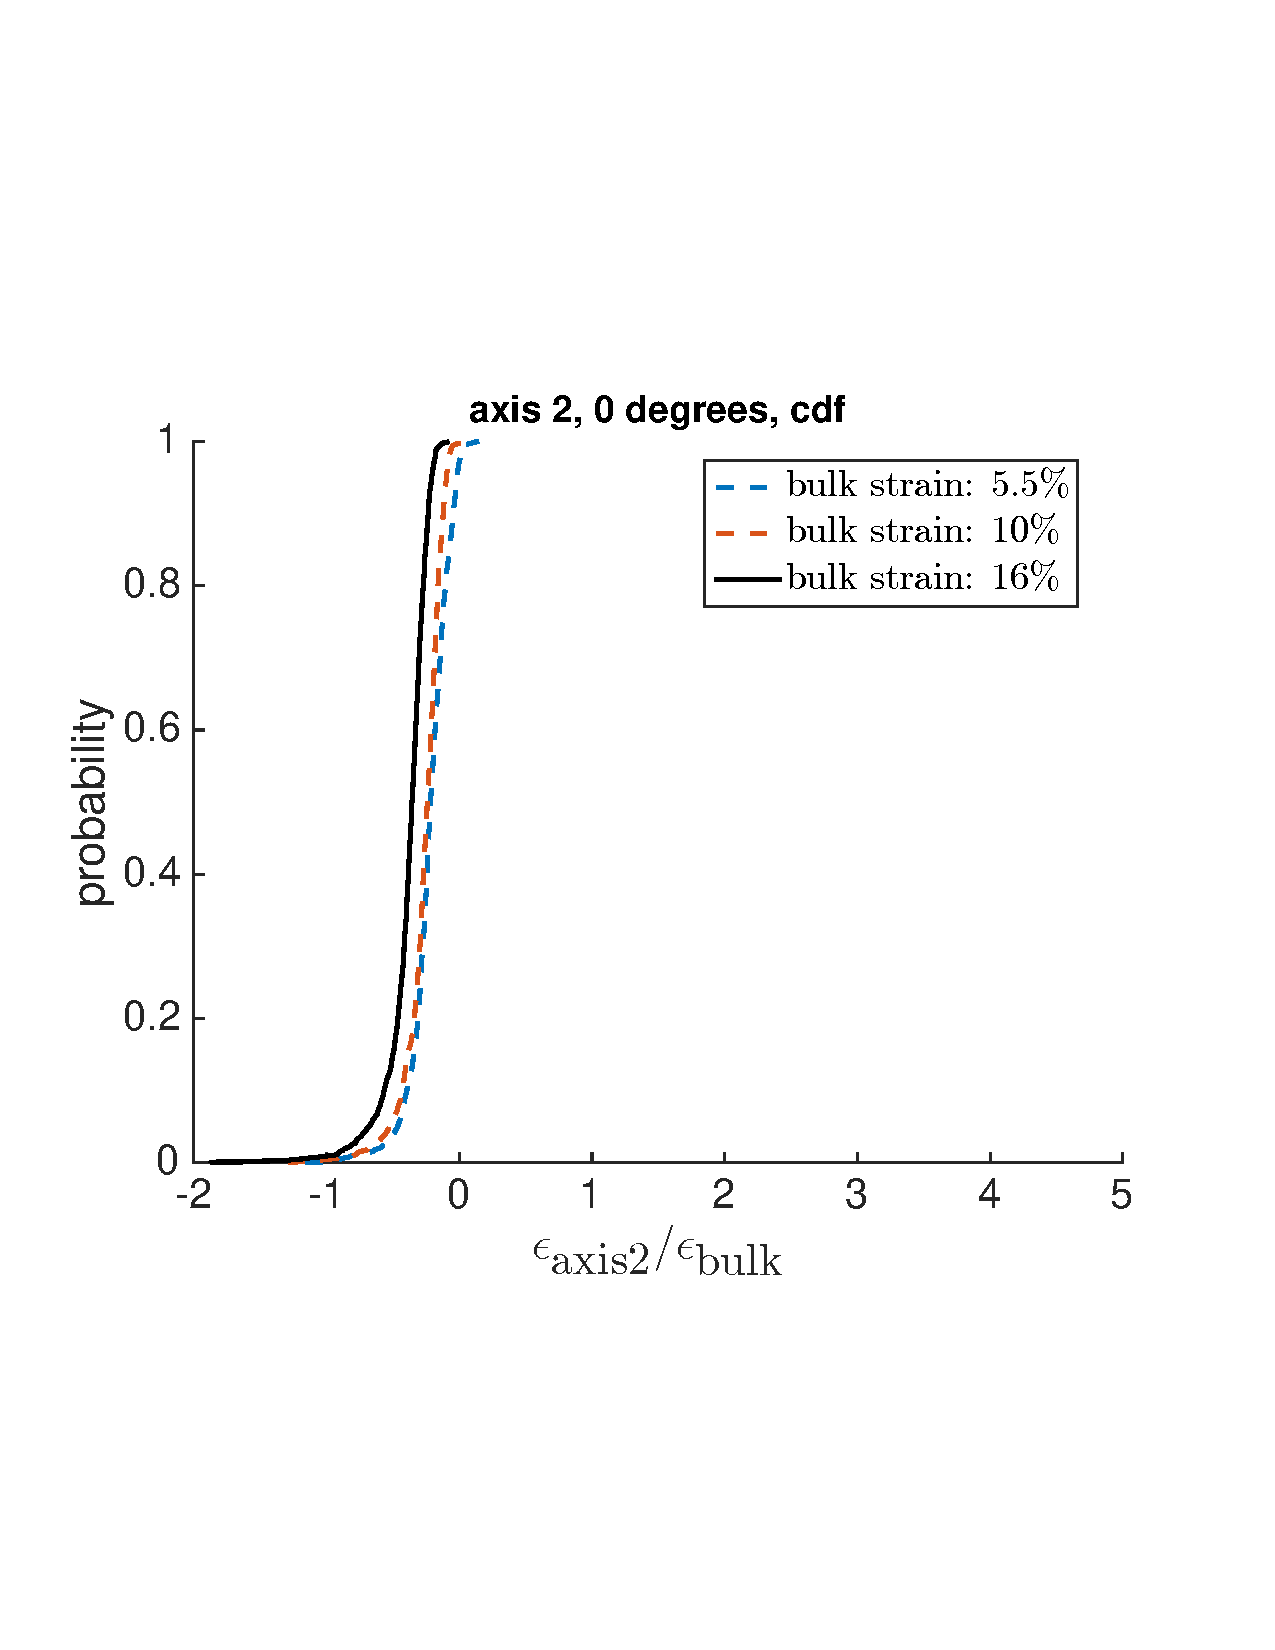
\includegraphics[height=4.5cm]{figure/rot0_FT50_strn22_128_1920_axial_cdf_axis1_compare_stps.pdf} & 
%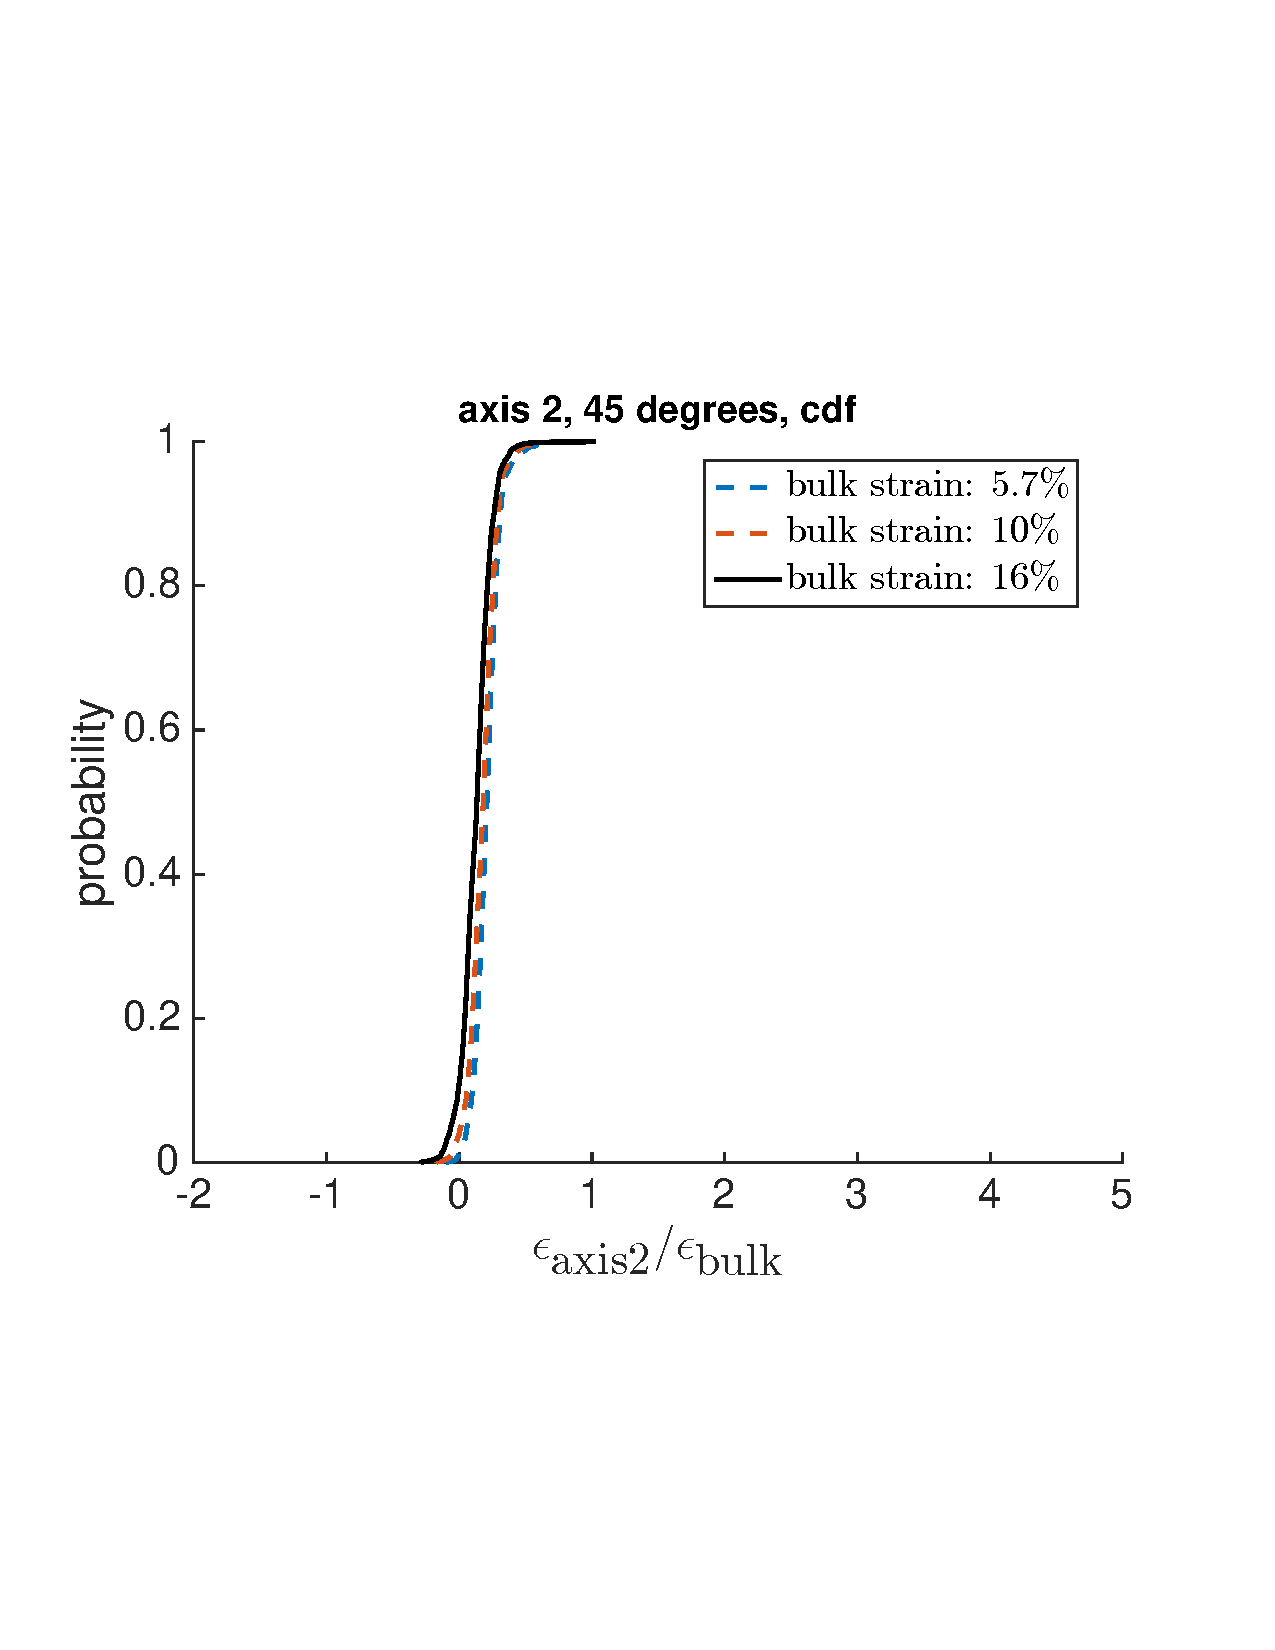
\includegraphics[height=4.5cm]{figure/rot45_FT50_strn22_128_1920_axial_cdf_axis1_compare_stps.pdf} & 
%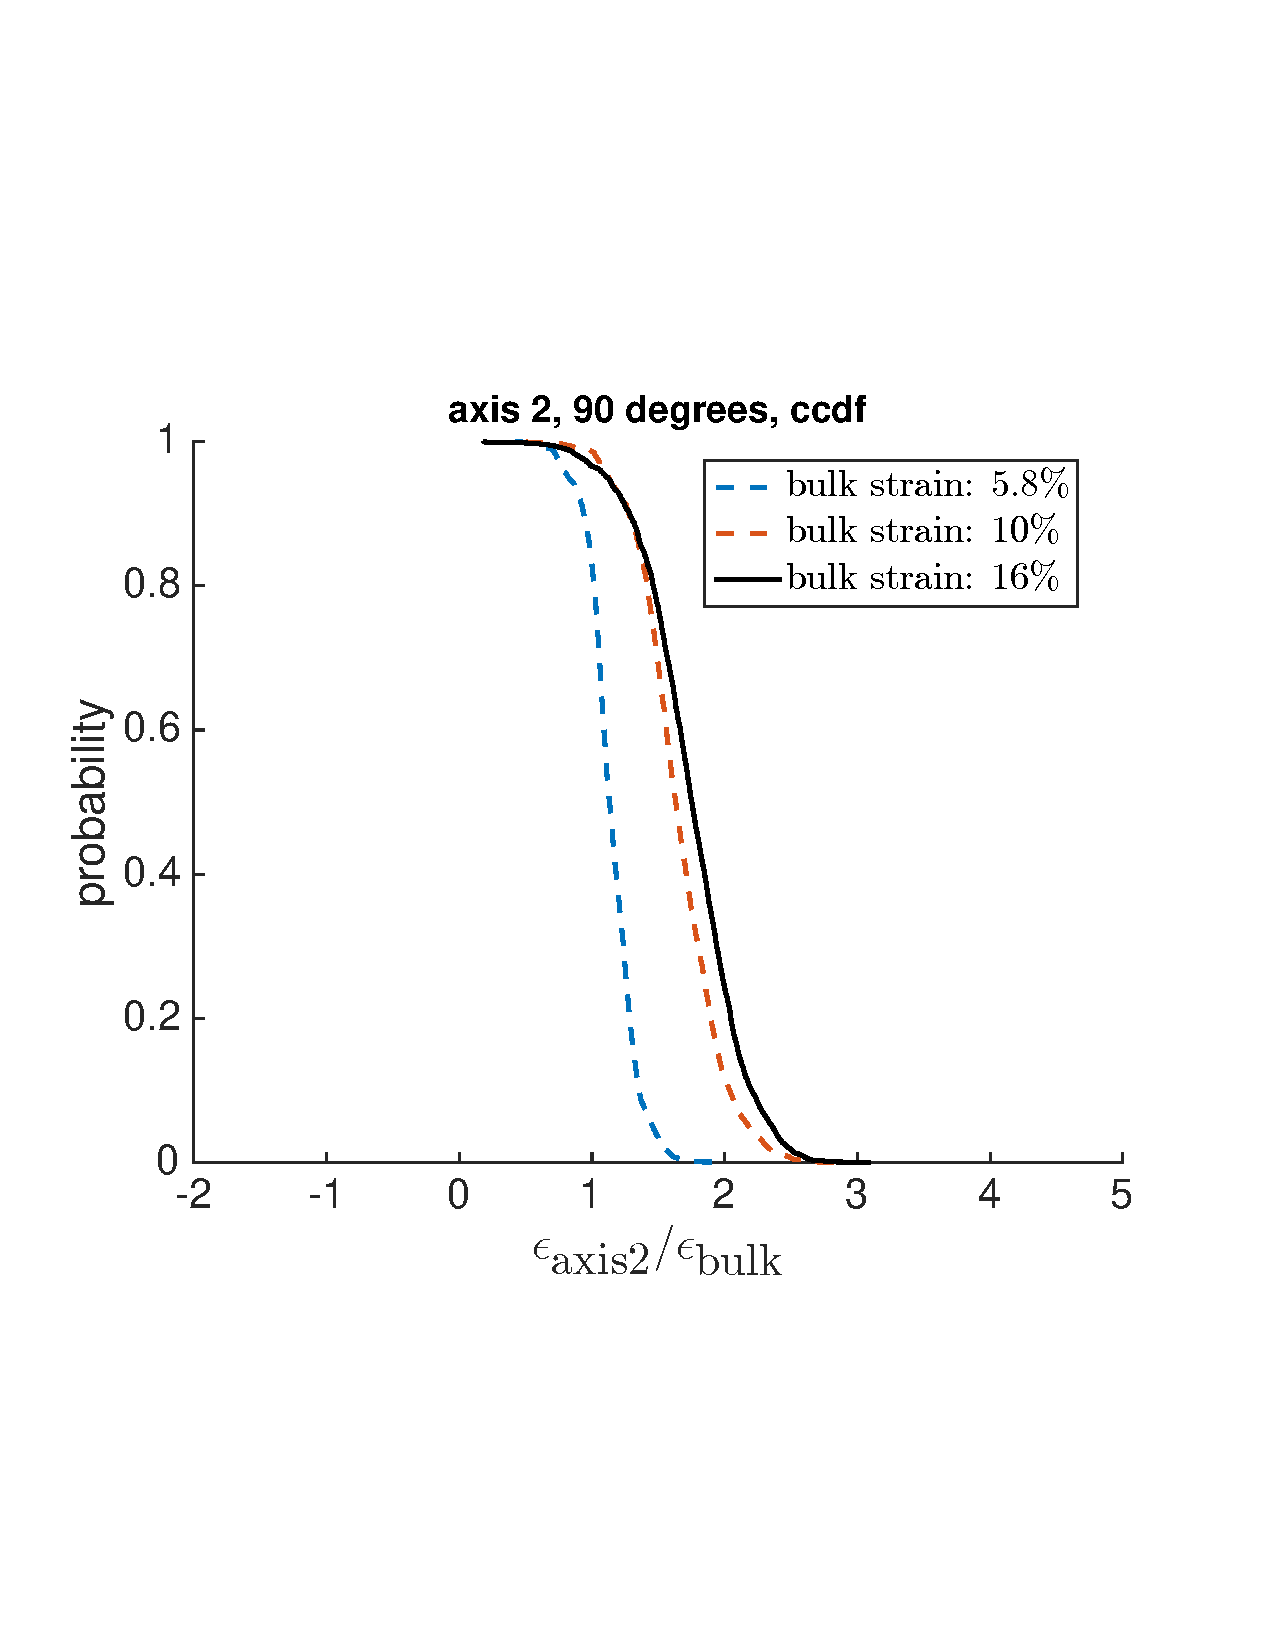
\includegraphics[height=4.5cm]{figure/rot90_FT50_strn22_ptdata_128_1920_axial_ccdf_axis1_compare_stps.pdf} \\
%(d) & (e) & (f) \\
%\end{array}
%$
%\end{center}
%\caption{\label{fig:axial_distr} Distributions of axial strain along axis 1 (top row) and axis 2 (bottom row) for different loading angles. The ccdf is plotted for tensile strains, while the cdf is plotted for compressive strains. For each loading angle, distributions for bulk strains of 5 - 6 $\%$ (dashed blue line), 10$\%$ (dashed red line), and 16$\%$ (solid black line) are plotted. The values of axial strain ($\epsilon_{\text{axis1}}$ or $\epsilon_{\text{axis2}}$) are normalized by the bulk strain, $\epsilon_{\text{bulk}}$.}
%\end{figure}
%%
%
%As seen in Fig.\ \ref{fig:axial_distr}, variations in the strain distributions are greatest for the 90 degree loading case where the amplification of local axial strain increases with increasing bulk strain - the distributions shift left and right for compressive and tensile strains, respectively. In contrast, only small variations are seen in the strain distributions for the 0 and 45 degree loading cases. 
%
%From a physiological stand point, the largest strains (i.e., the tails of the distributions) are most important because those are the regions where neuron damage arises. To understand how the high strain portions of the neuron structure relate to bulk strain applied to the gel, the local-strain amplification corresponding to the portion of the structure that experiences the largest 5$\%$ strain (0.05 on ordinate of distributions in Fig.\ \ref{fig:axial_distr}) are plotted as a function of bulk strain in Fig.\ \ref{fig:axial_amp}. 
%%
%% images are from N2P178/5-Neuron_LocalAxon_Strain/MaxPrnStrn/PlotStrnAmp.m
%\begin{figure}[ht]
%\begin{center}
%$
%\begin{array}{ccc}
%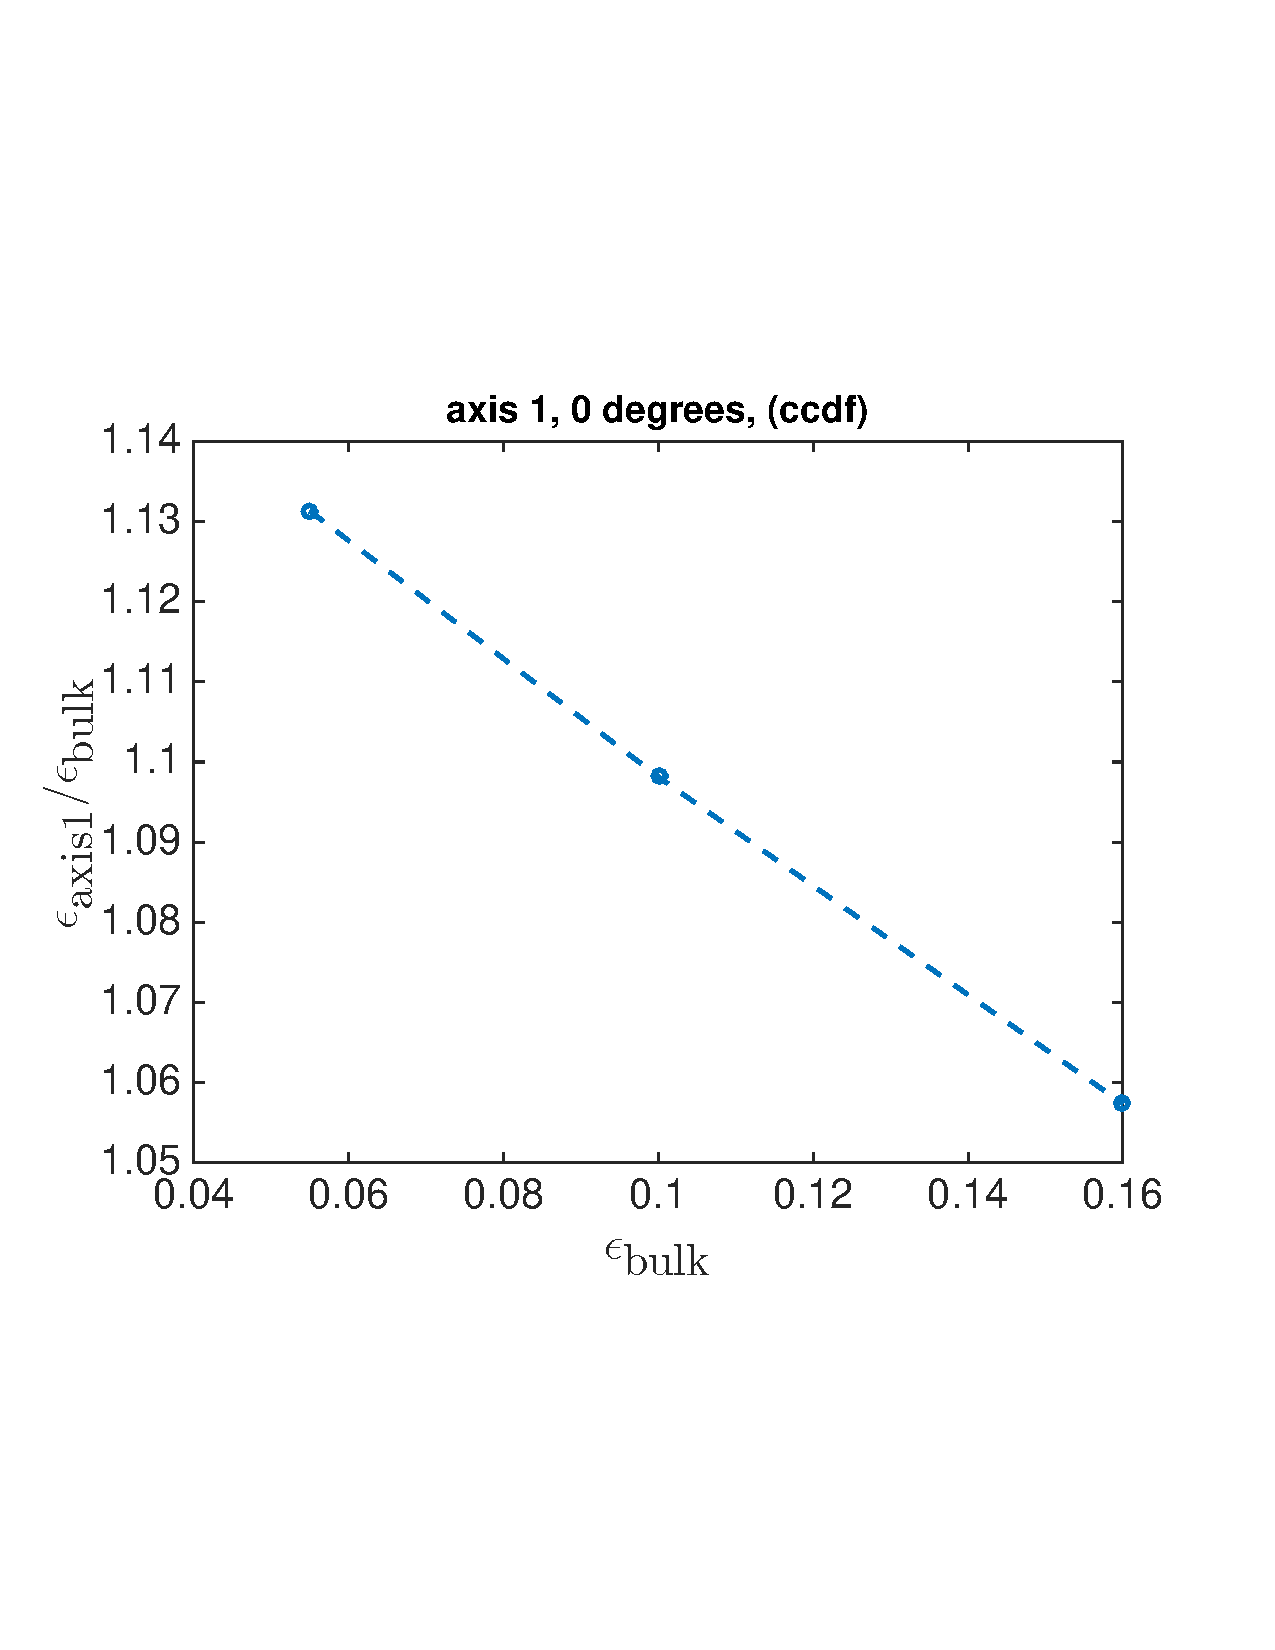
\includegraphics[height=4.5cm]{figure/rot0_FT50_strn11_128_1920_axial_ccdf_axis1_strn_amp.pdf} & 
%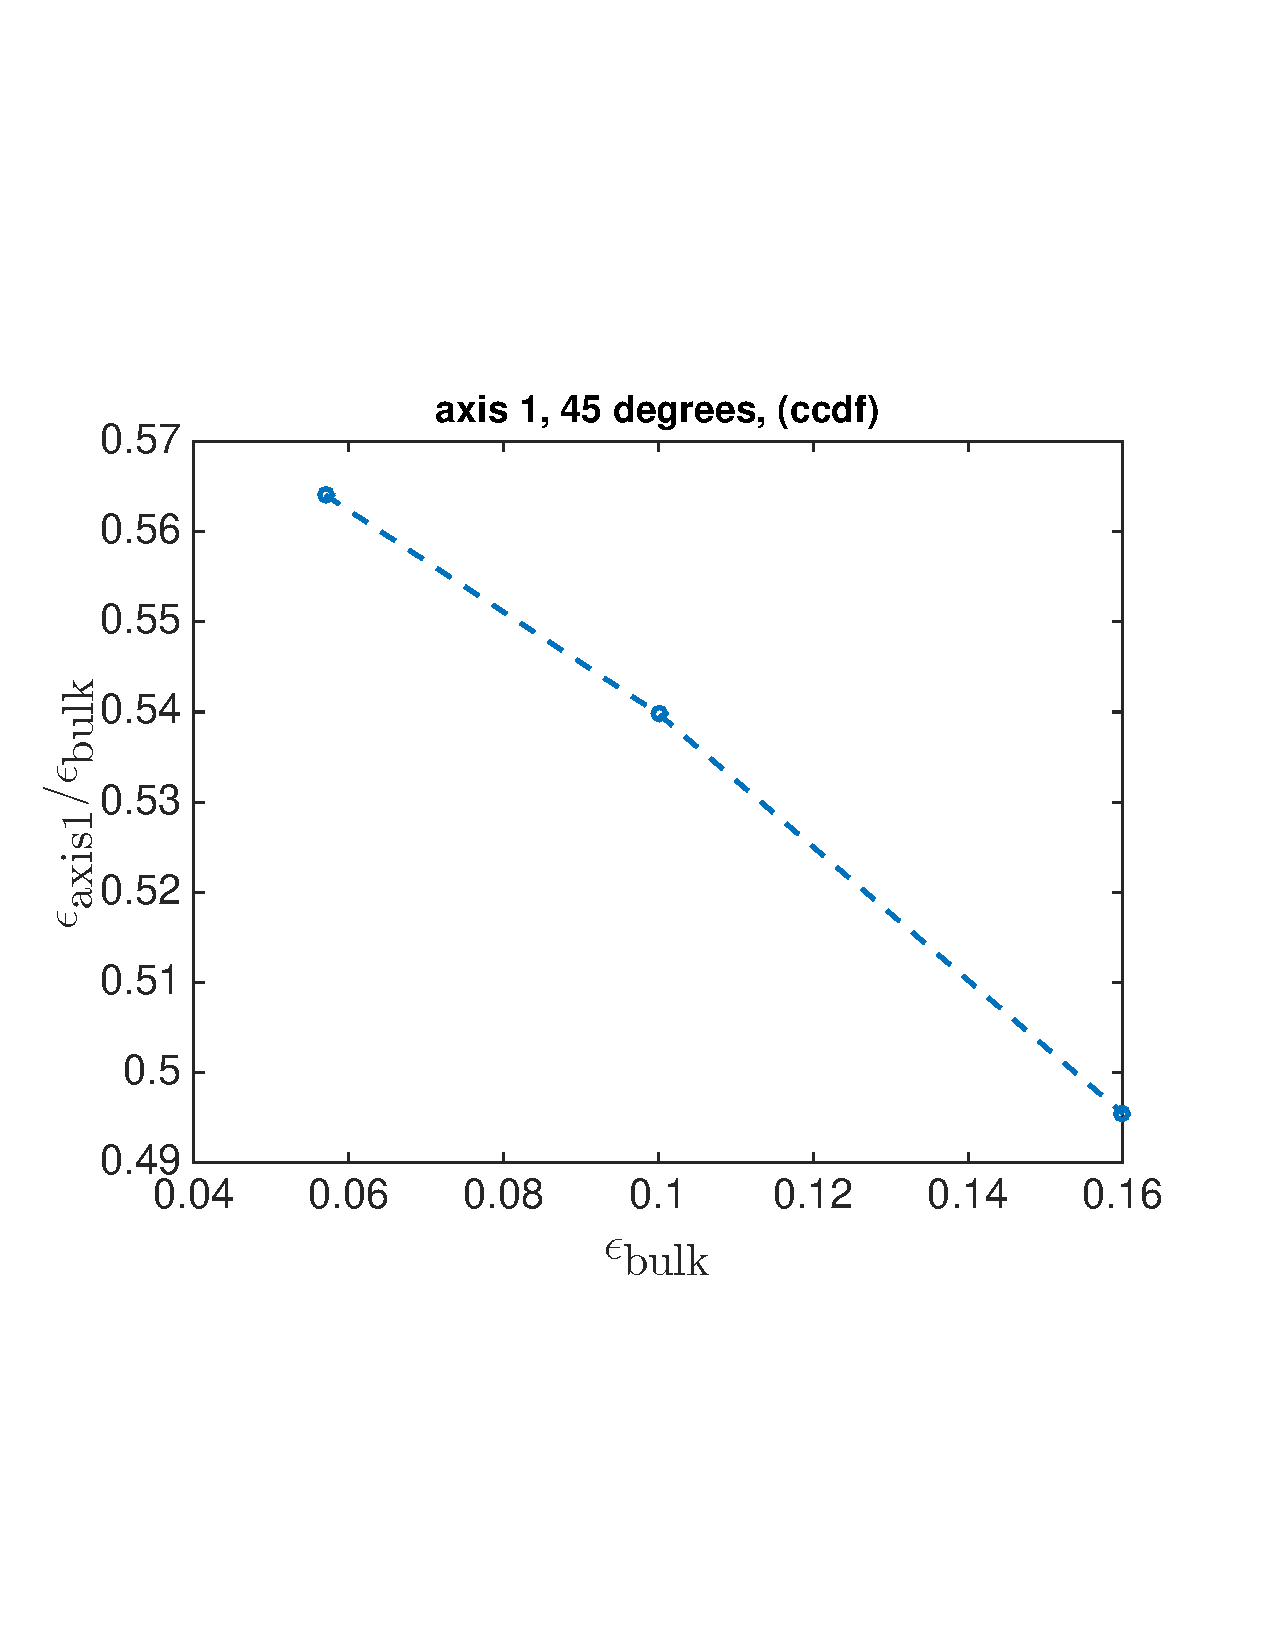
\includegraphics[height=4.5cm]{figure/rot45_FT50_strn11_128_1920_axial_ccdf_axis1_strn_amp.pdf} &
%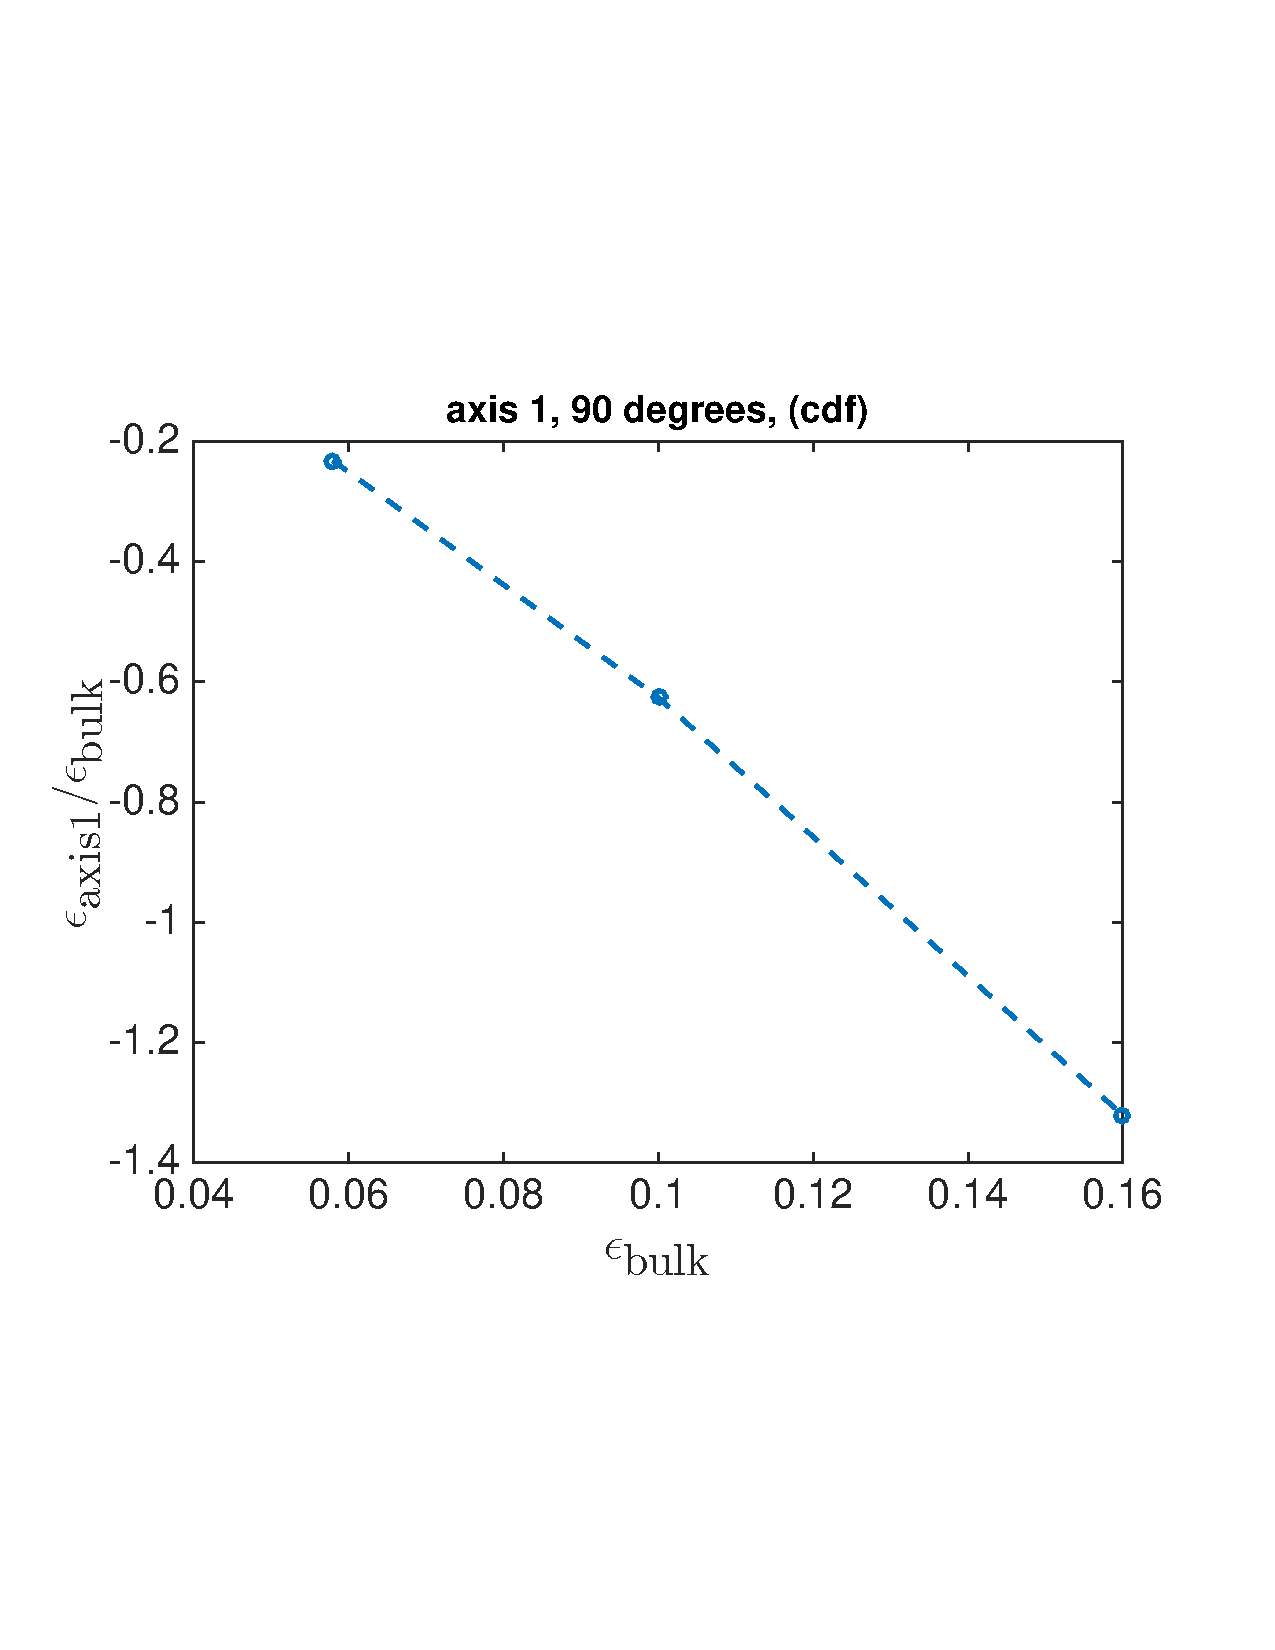
\includegraphics[height=4.5cm]{figure/rot90_FT50_strn11_128_1920_axial_cdf_axis1_strn_amp.pdf} \\
%(a) & (b) & (c) \\ 
%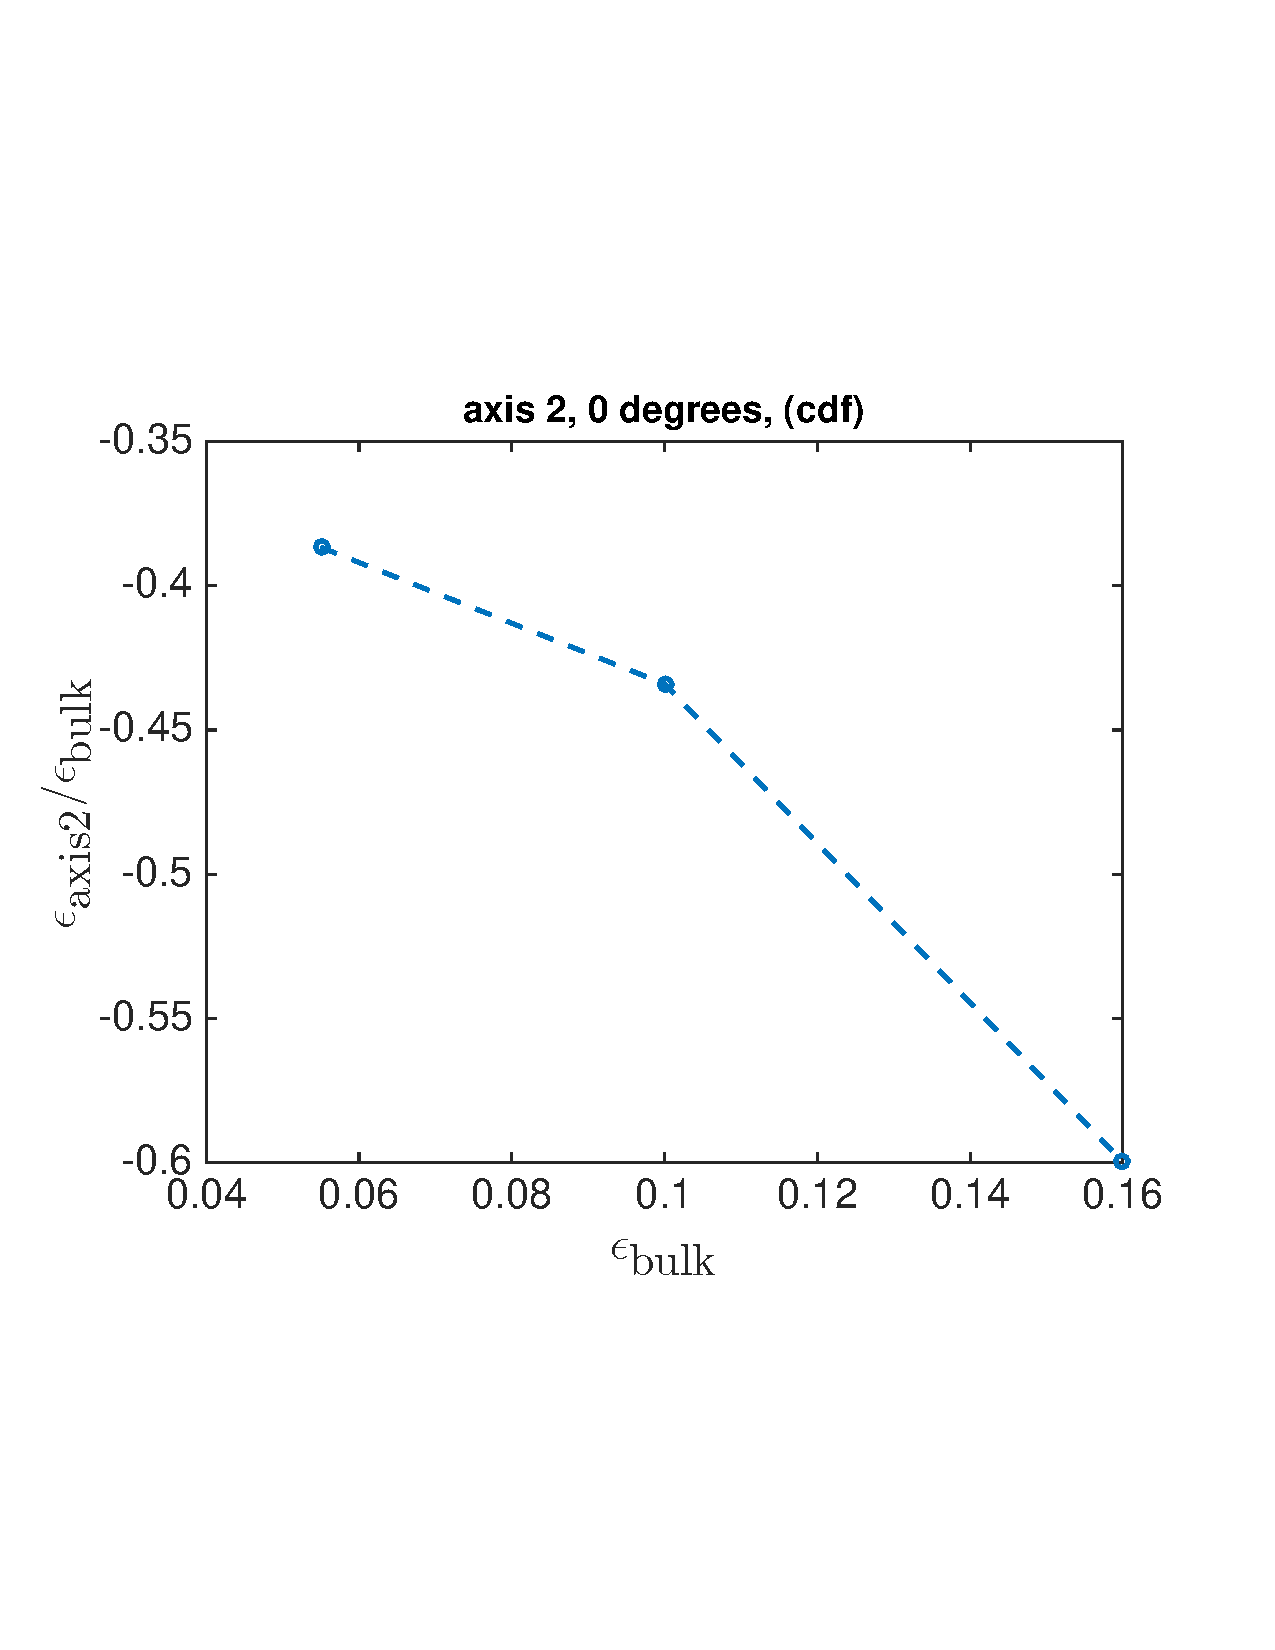
\includegraphics[height=4.5cm]{figure/rot0_FT50_strn22_128_1920_axial_cdf_axis1_strn_amp.pdf} &
%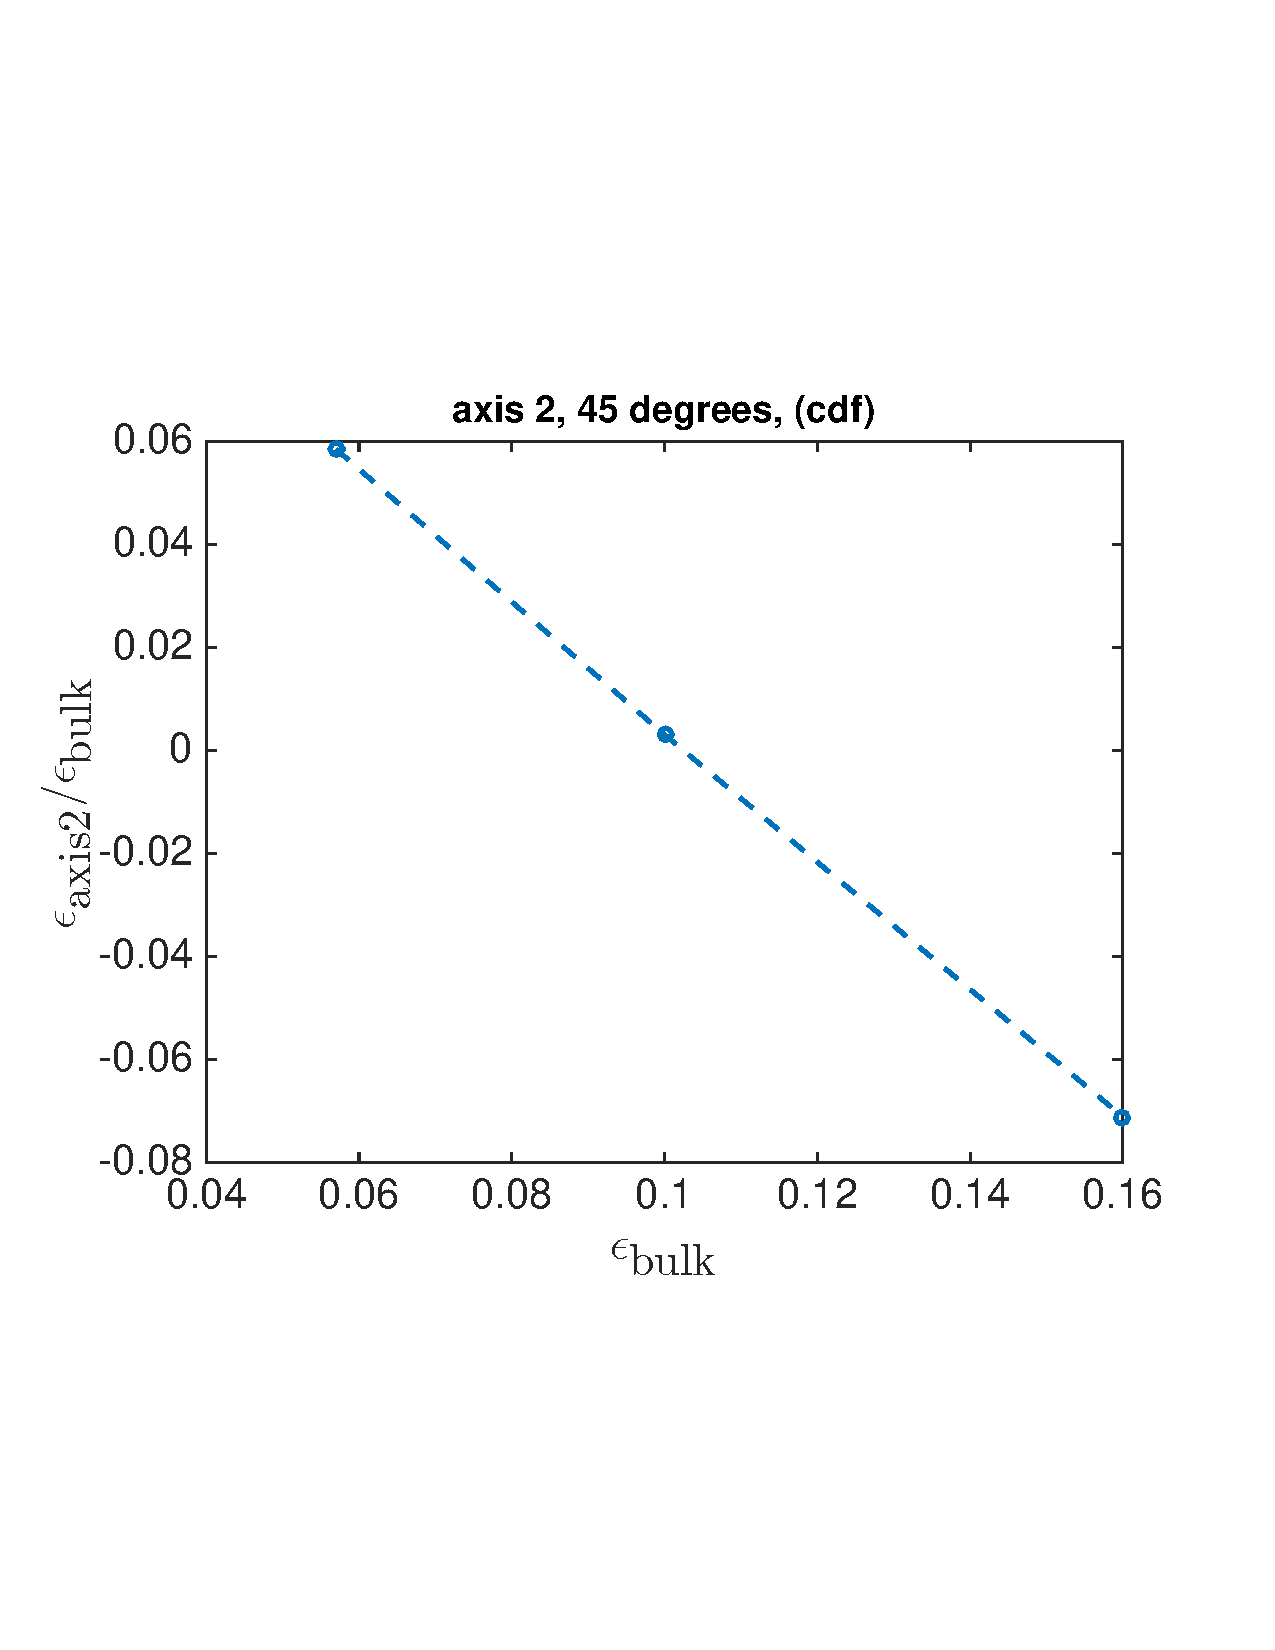
\includegraphics[height=4.5cm]{figure/rot45_FT50_strn22_128_1920_axial_cdf_axis1_strn_amp.pdf} & 
%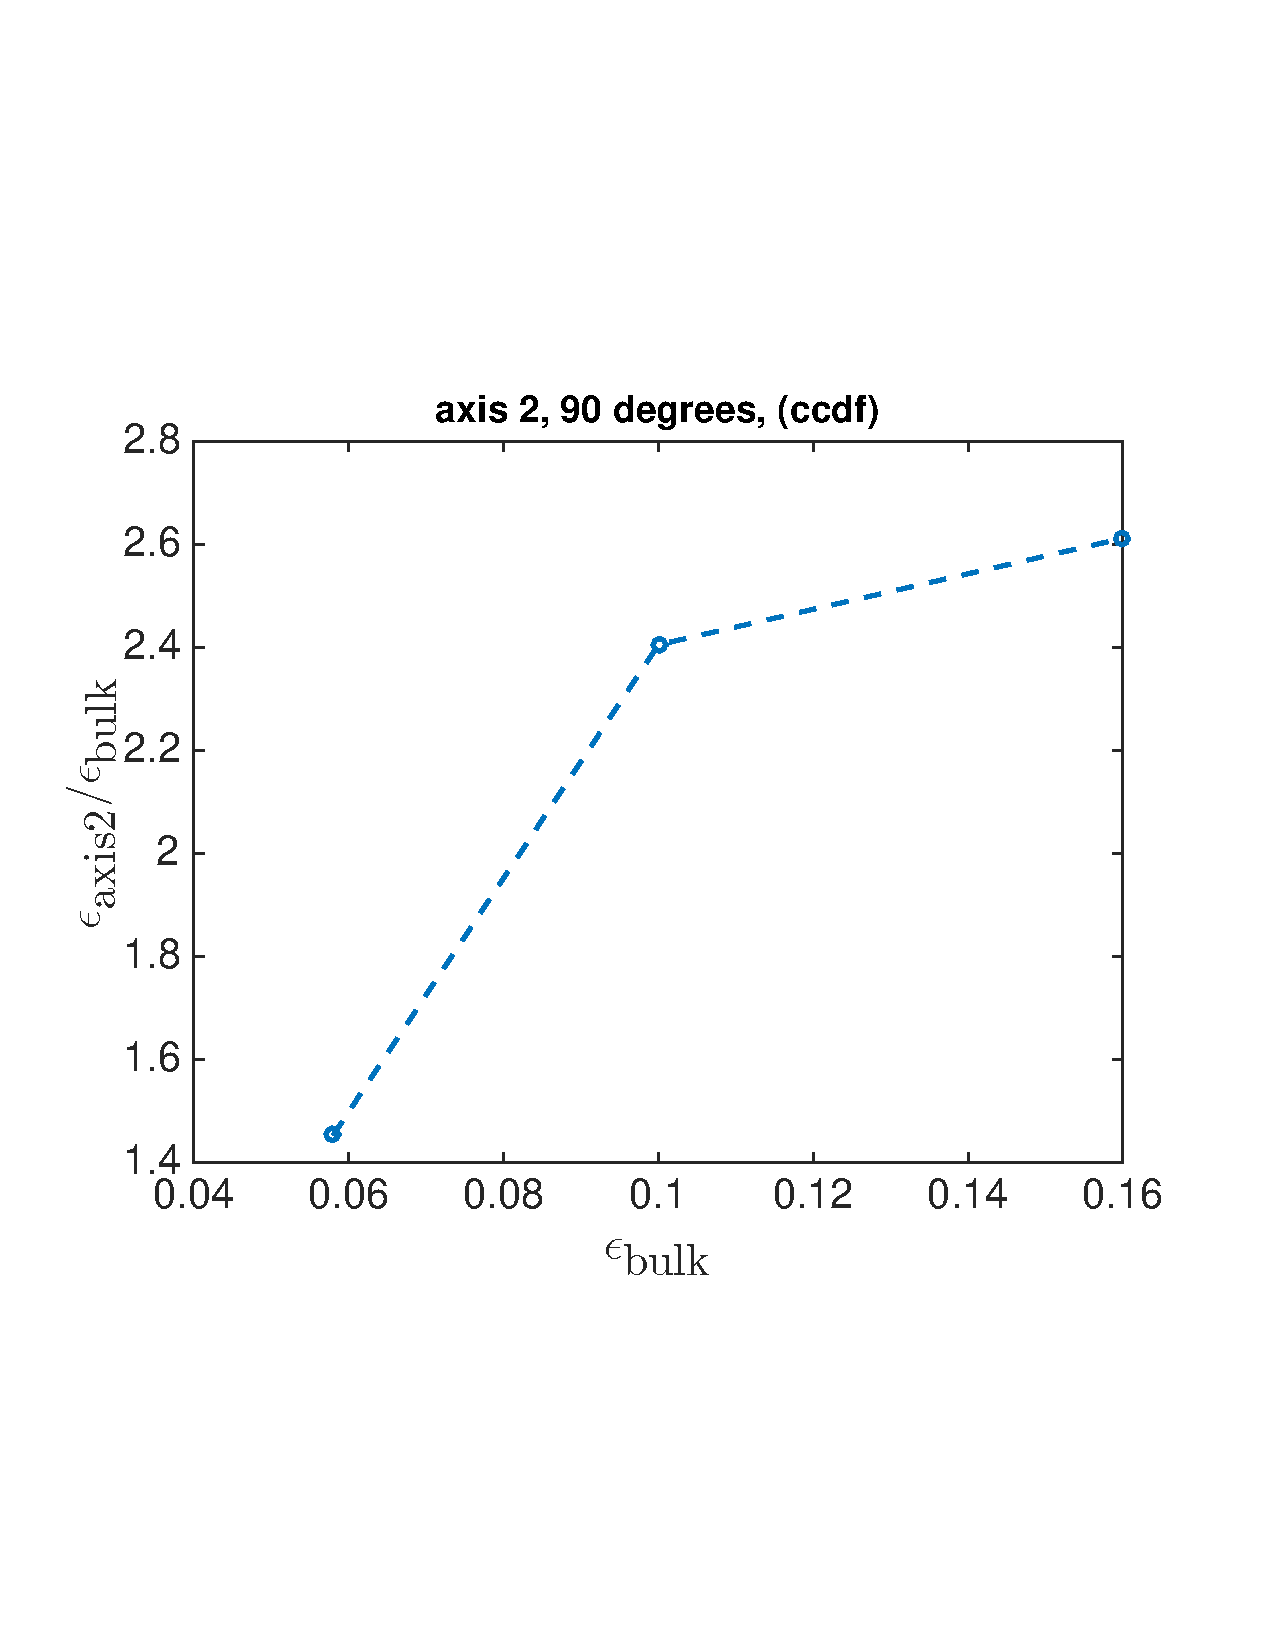
\includegraphics[height=4.5cm]{figure/rot90_FT50_strn22_128_1920_axial_ccdf_axis1_strn_amp.pdf} \\
%(d) & (e) & (f) 
%\end{array}
%$
%\end{center}
%\caption{\label{fig:axial_amp} Local strain amplification corresponding to the portion of the neuron structure in Fig.\ \ref{fig:axial_schematic} that experiences the largest 5$\%$ strain (0.05 on ordinate of distributions in Fig.\ \ref{fig:axial_distr}) as a function of bulk strain for different loading directions.}
%\end{figure}
%%
%
%As seen in Fig.\ \ref{fig:axial_amp}, the local-strain amplification of the lateral compressive strains increase for all loading angles - axis 2 for 0 and 45 degree loading and axis 1 for 90 degree loading. This is consistent with the fact that the Poisson ratio of the collagen gel increases with larger deformations (see Poisson ratio curve in Fig.\ \ref{fig:fiber_param2}(a)). Note that for 45 degree loading, axis 2 experiences tensile strains at smaller bulk strains before the lateral compressive strains that arise from the Poisson ratio effect become large enough to dominate. Interestingly, the local-strain amplification of the tensile strain decreases for the 0 and 45 degree loading cases and increases for the 90 degree loading cases - axis 1 for 0 and 45 degree loading and axis 2 for 90 degree loading. This result suggests that a configuration where the axial direction of the neuron is near parallel to the loading direction (e.g., axis 1 for 0 and 45 degree loading cases) is more favorable than a configuration where the axial direction of the neuron is near orthogonal to the loading direction (e.g., axis 2 for the 90 degree loading case). The underlying mechanisms for such behavior is explored in the next section.

%%%%%%%%%%%%%%%%%%%%%%%%%%%%%%%%%%%%%%%%%%%%%%%%%%%%%%%%%%%%%%%%%%%%%%
\section{Discussion}

The results in Sections \ref{sec:cellbody_stiffness} and \ref{sec:loading_direction} illustrate that the strain distribution (ccdf) in the neuron structure, and hence strain amplification, is most strongly influenced by the configuration of the neuron with respect to the loading direction. The strong dependence of the strain distribution on loading configuration reflects the anisotropic nature of the embedded neuron structure, where the axial stiffness is an order of magnitude stiffer than the transverse stiffness. Relative to the stiffness of the surrounding collagen gel, the axial stiffness of the neuron is larger while the transverse stiffness of the neuron is smaller. Due to the complex geometry of the embedded neuron structure studied above, the neuron is exposed to both transverse and axial components of loading. The spread of ccdfs reflects the range of tranverse and axial loads that different regions within the neuron is exposed to.

At one extreme when the load on the neuron is purely transverse, strain amplification arises because the transverse stiffness of the neuron is lower than that of the collagen gel. The strain amplification is intensified by the stiffening of the surrounding collagen gel during deformation, which effectively softens the neuron relative to the collagen gel. Combined, the transverse loading in the neuron and the stiffening of the collagen gel causes the strain amplification in the neuron to grow as the deformation in the surrounding collagen gel increases. At the other extreme when the load on the neuron is purely axial, the strain experienced by the neuron is less than that in the gel because the axial stiffness of the neuron is greater than that of the collagen gel. The strain discrepancy between the neuron and gel decreases with deformation due to the stiffening of the collagen gel. 

In the 90 degree loading configuration, the neuron is exposed to primarily transverse loading, giving rise to large strain amplification in the neuron. For example, as seen in the ccdf of Fig.\ \ref{fig:neuron_ccdf_mps}(d), the average MPS in the neuron is more than twice as large as the bulk strain in the surrounding gel, while the maximum MPS (tail of ccdf) in the neuron is six times larger than the applied load on the surrounding gel. Furthermore, the average and maximum MPS in the neuron for 90 degree loading increases with bulk strain in the collagen gel (comparing Figs.\ \ref{fig:neuron_ccdf_mps}(c) and (d)), which reflects the neuron becoming relatively softer due the stiffening of the surrounding gel. 

In the 0 and 45 degree loading configurations, the neuron is exposed more prominently to axial loading resulting in lower strain amplifications. Comparing the two loading cases, the spread of the ccdfs for 0 degree loading (Figs.\ \ref{fig:neuron_ccdf_0deg_mps}) is wider indicating a less uniform loading on the structure. Physiologically more significant, the tail of the of the ccdfs for 0 degree loading are longer indicating larger strain amplification in the neuron and hence a higher potential for injury in the neuron. Interestingly, the tail of the ccdfs for 0 degree loading decreases with bulk strain in the collagen gel (comparing Figs.\ \ref{fig:neuron_ccdf_0deg_mps}(a) and (b)), which reflects a ``self correcting" mechanism where the neuron structure aligns axially with the direction of loading. This self correcting behavior is opposite of what is seen in the 90 degree loading case suggesting that the axial alignment of the neuron takes place more rapidly than the stiffening of the collagen gel.

%\subsection{Fiber Alignment in Collagen Gel}
%%
%\begin{figure}[ht]
%\begin{center}
%$
%\begin{array}{ccc}
%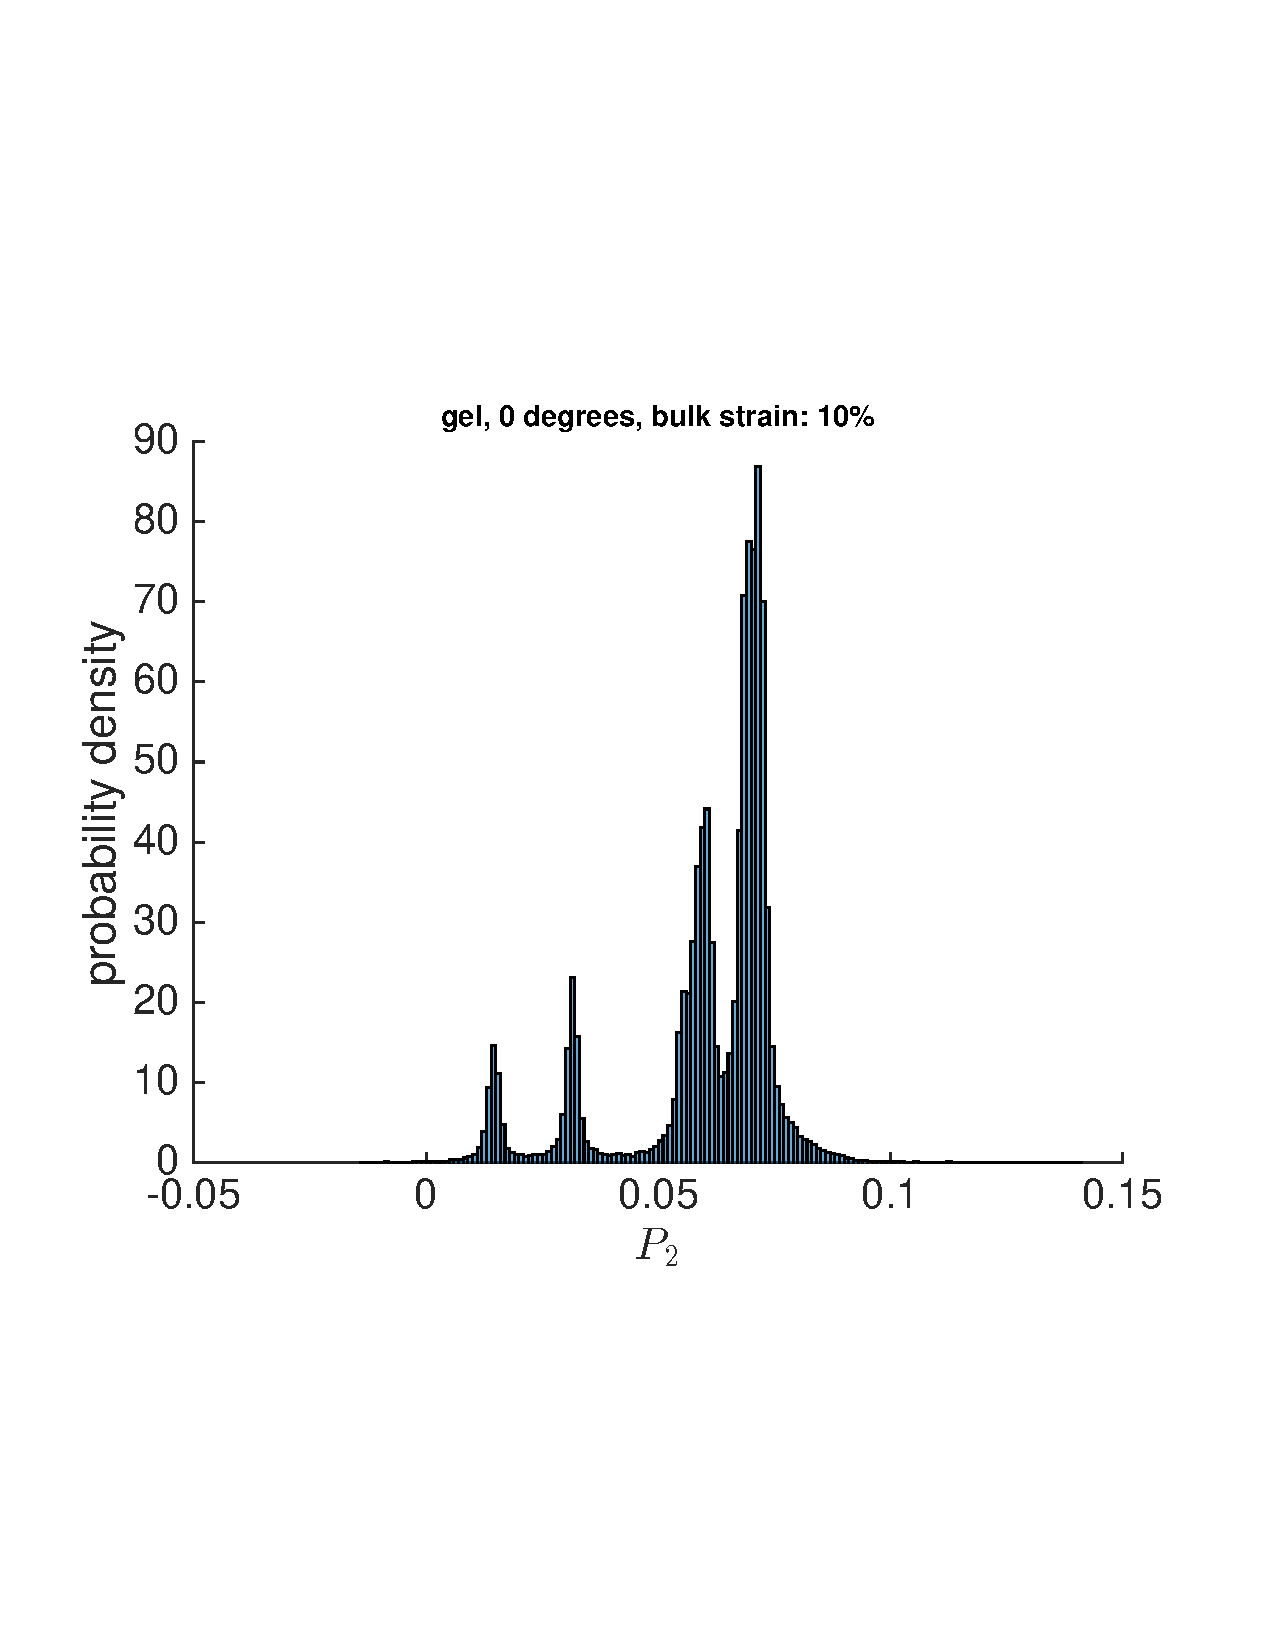
\includegraphics[height=4cm]{figure/rot0_FT50_128_1920_histo_gel_5.pdf} & 
%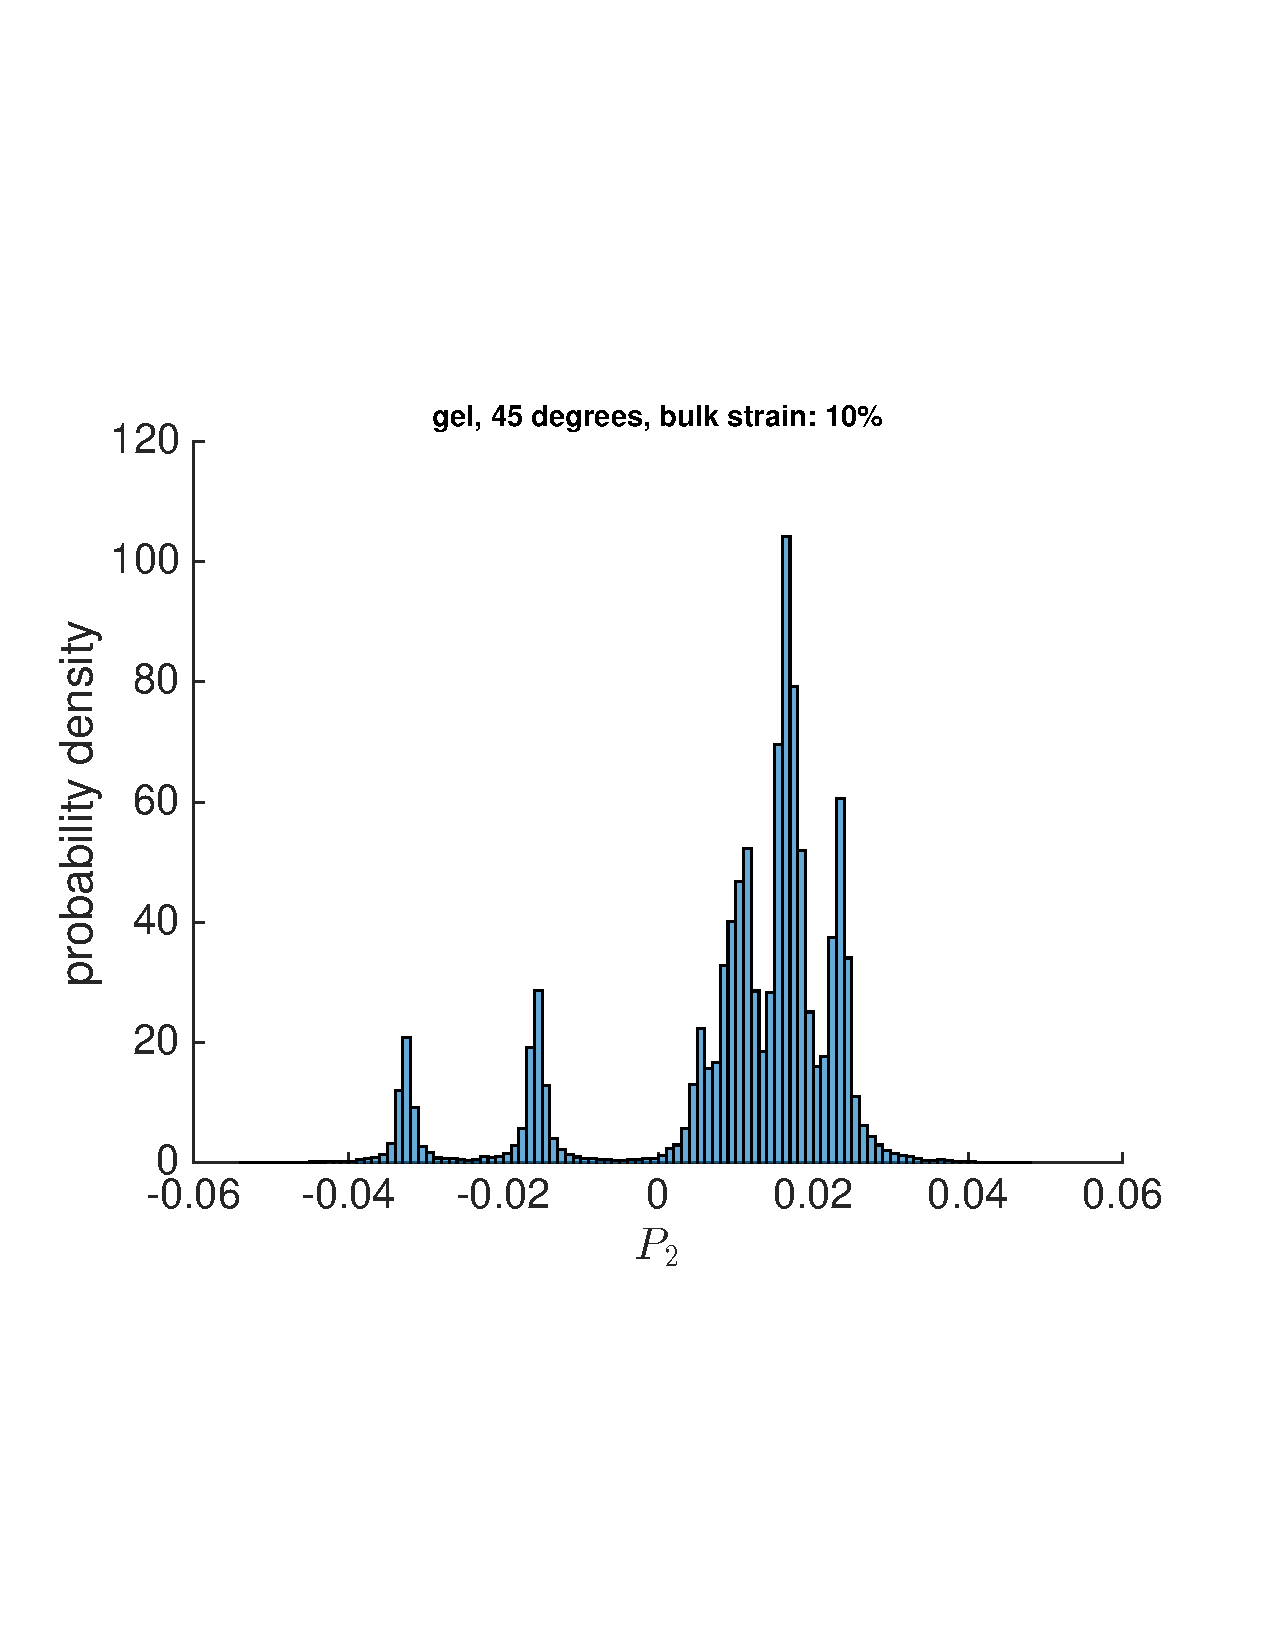
\includegraphics[height=4cm]{figure/rot45_FT50_128_1920_histo_gel_8.pdf} &
%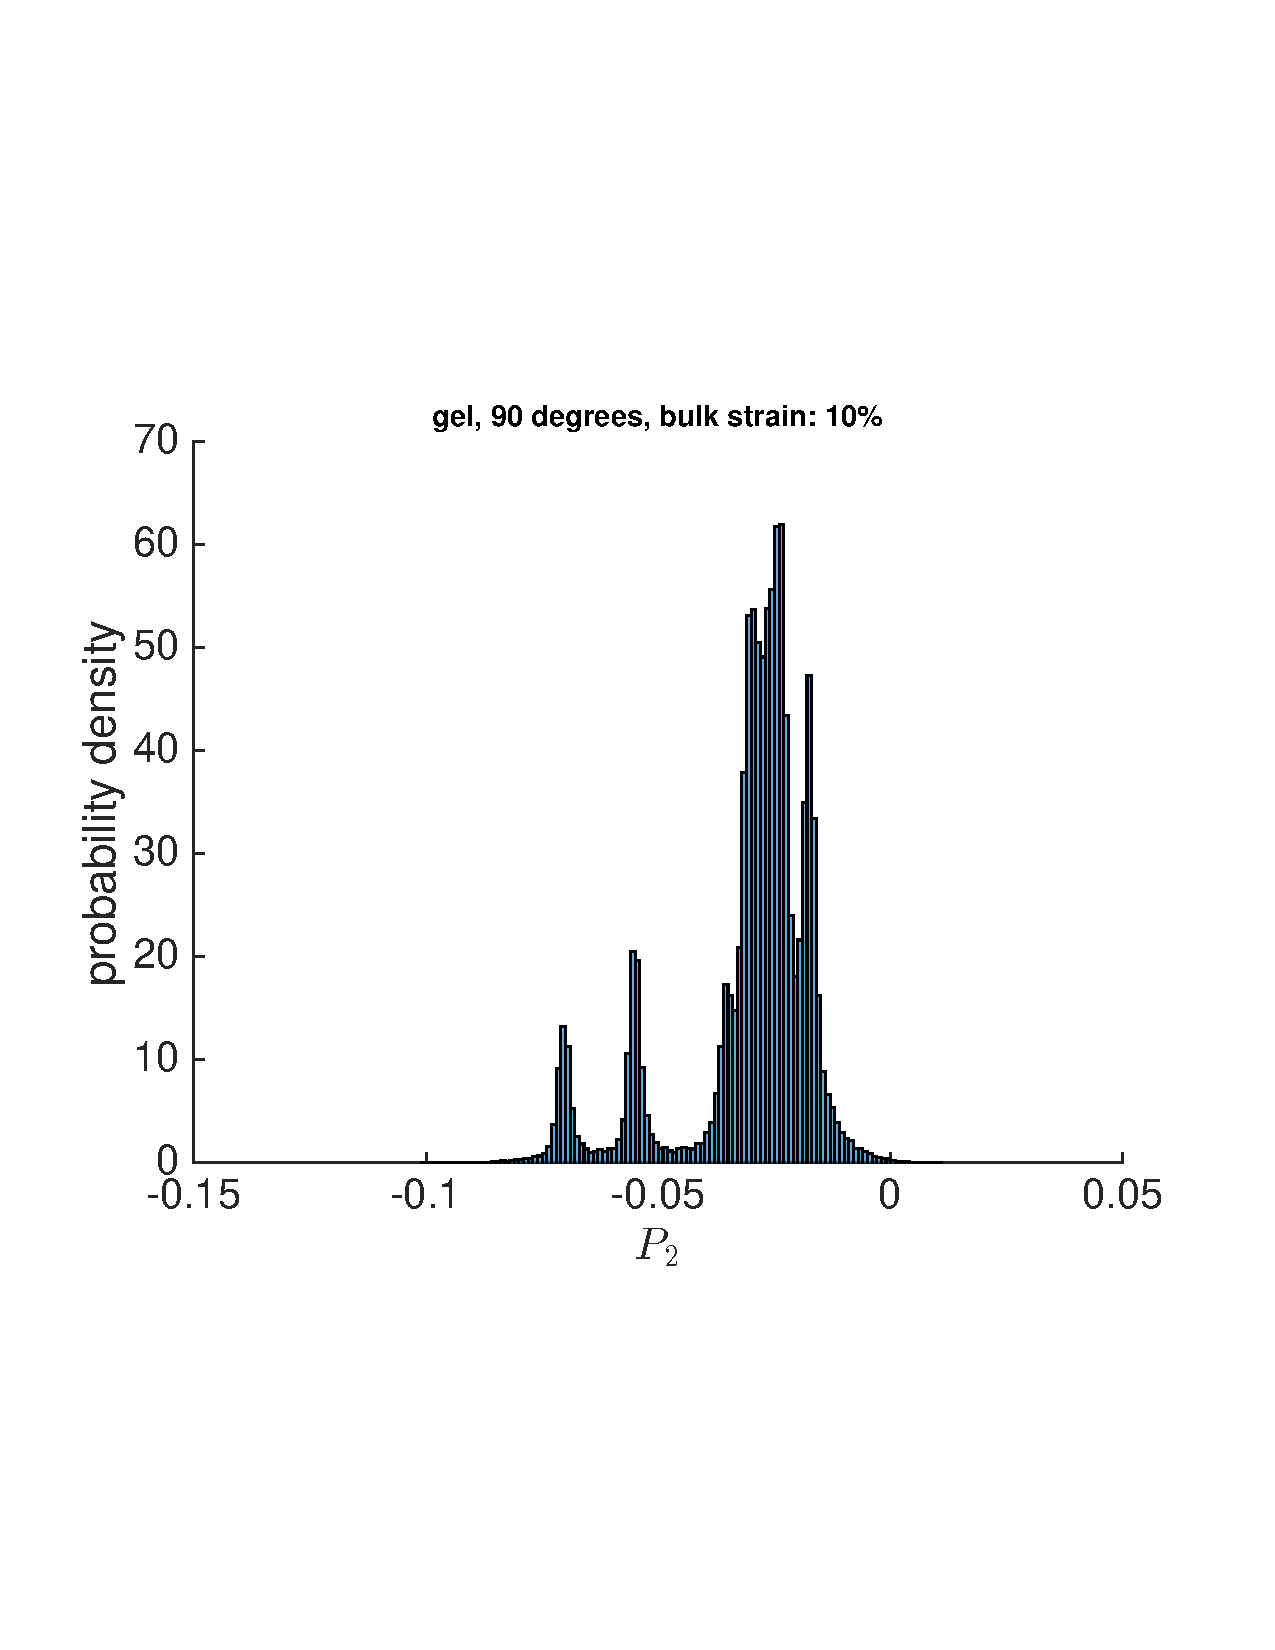
\includegraphics[height=4cm]{figure/rot90_FT_dspBC50_a30_128_1920_histo_gel_27.pdf} \\
%(a) & (b) & (c) \\ 
%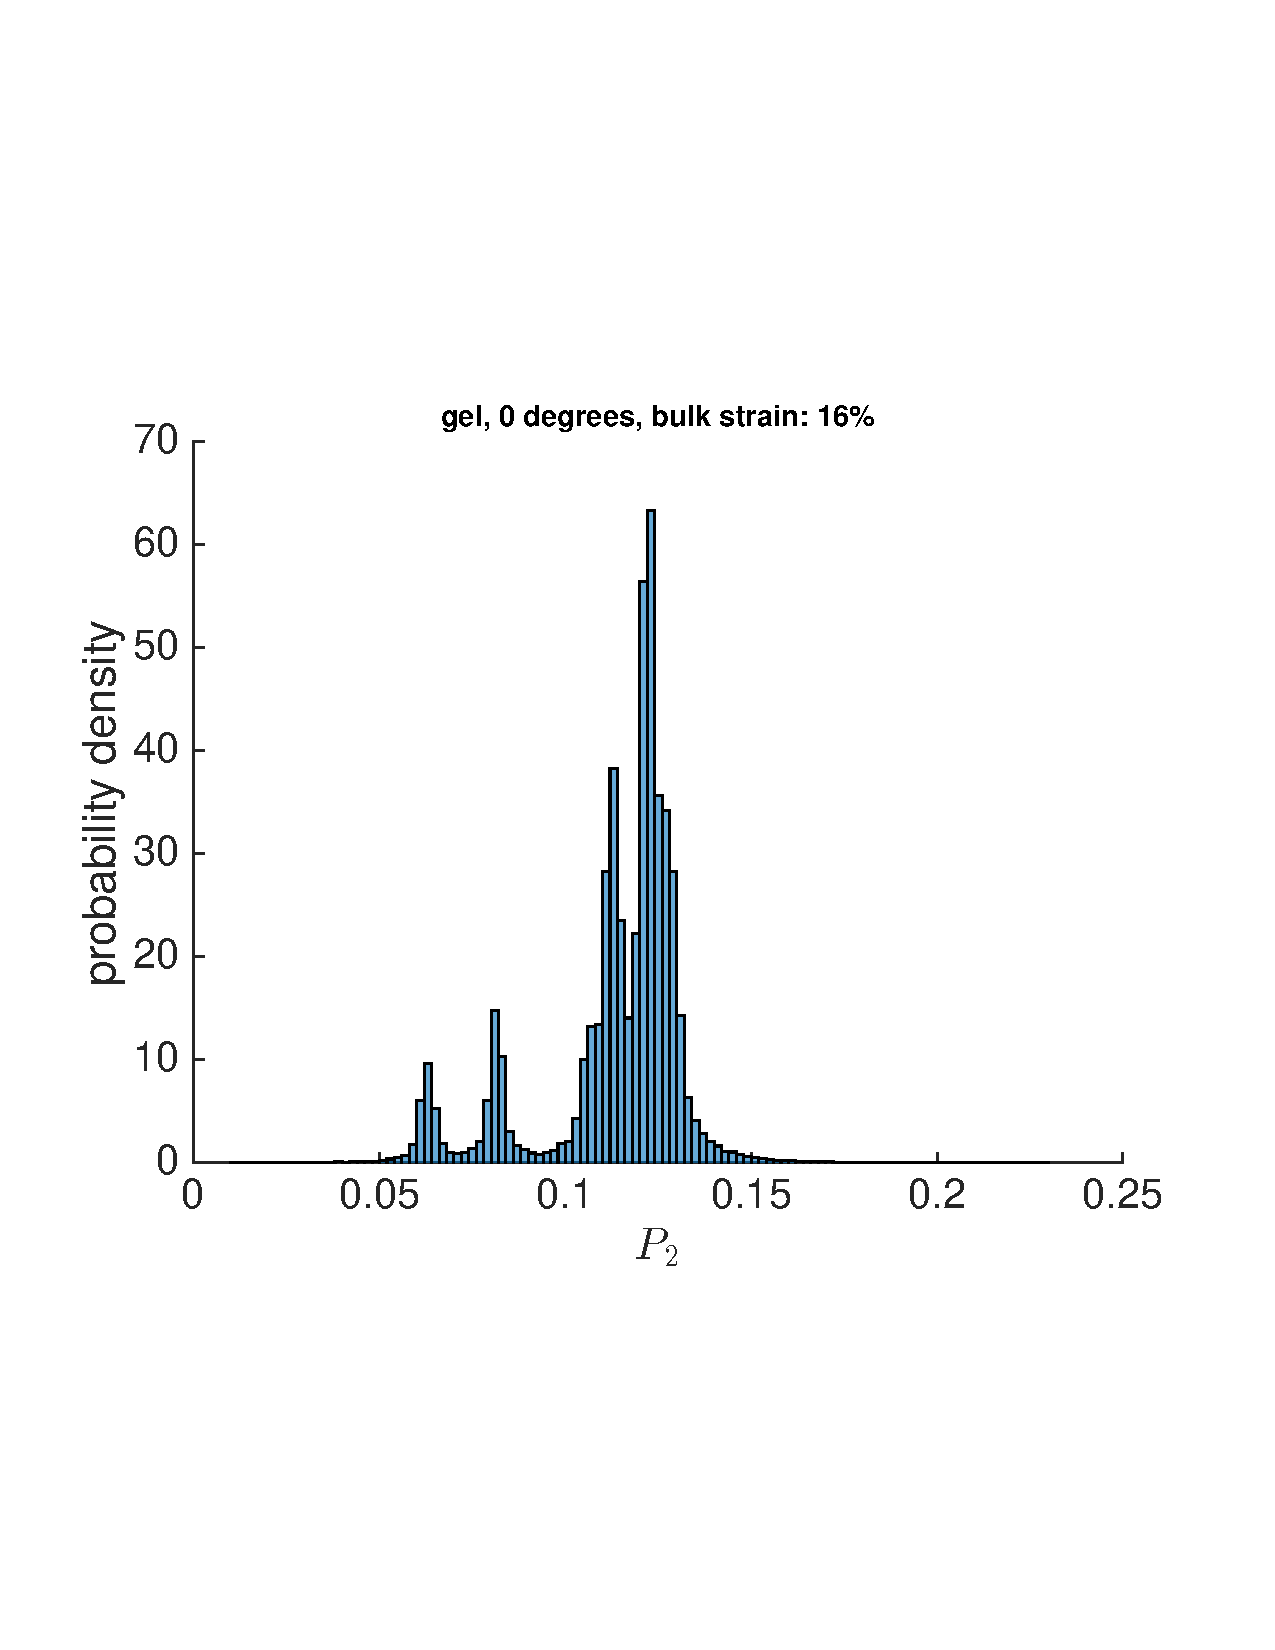
\includegraphics[height=4cm]{figure/rot0_FT50_128_1920_histo_gel_20.pdf} &
%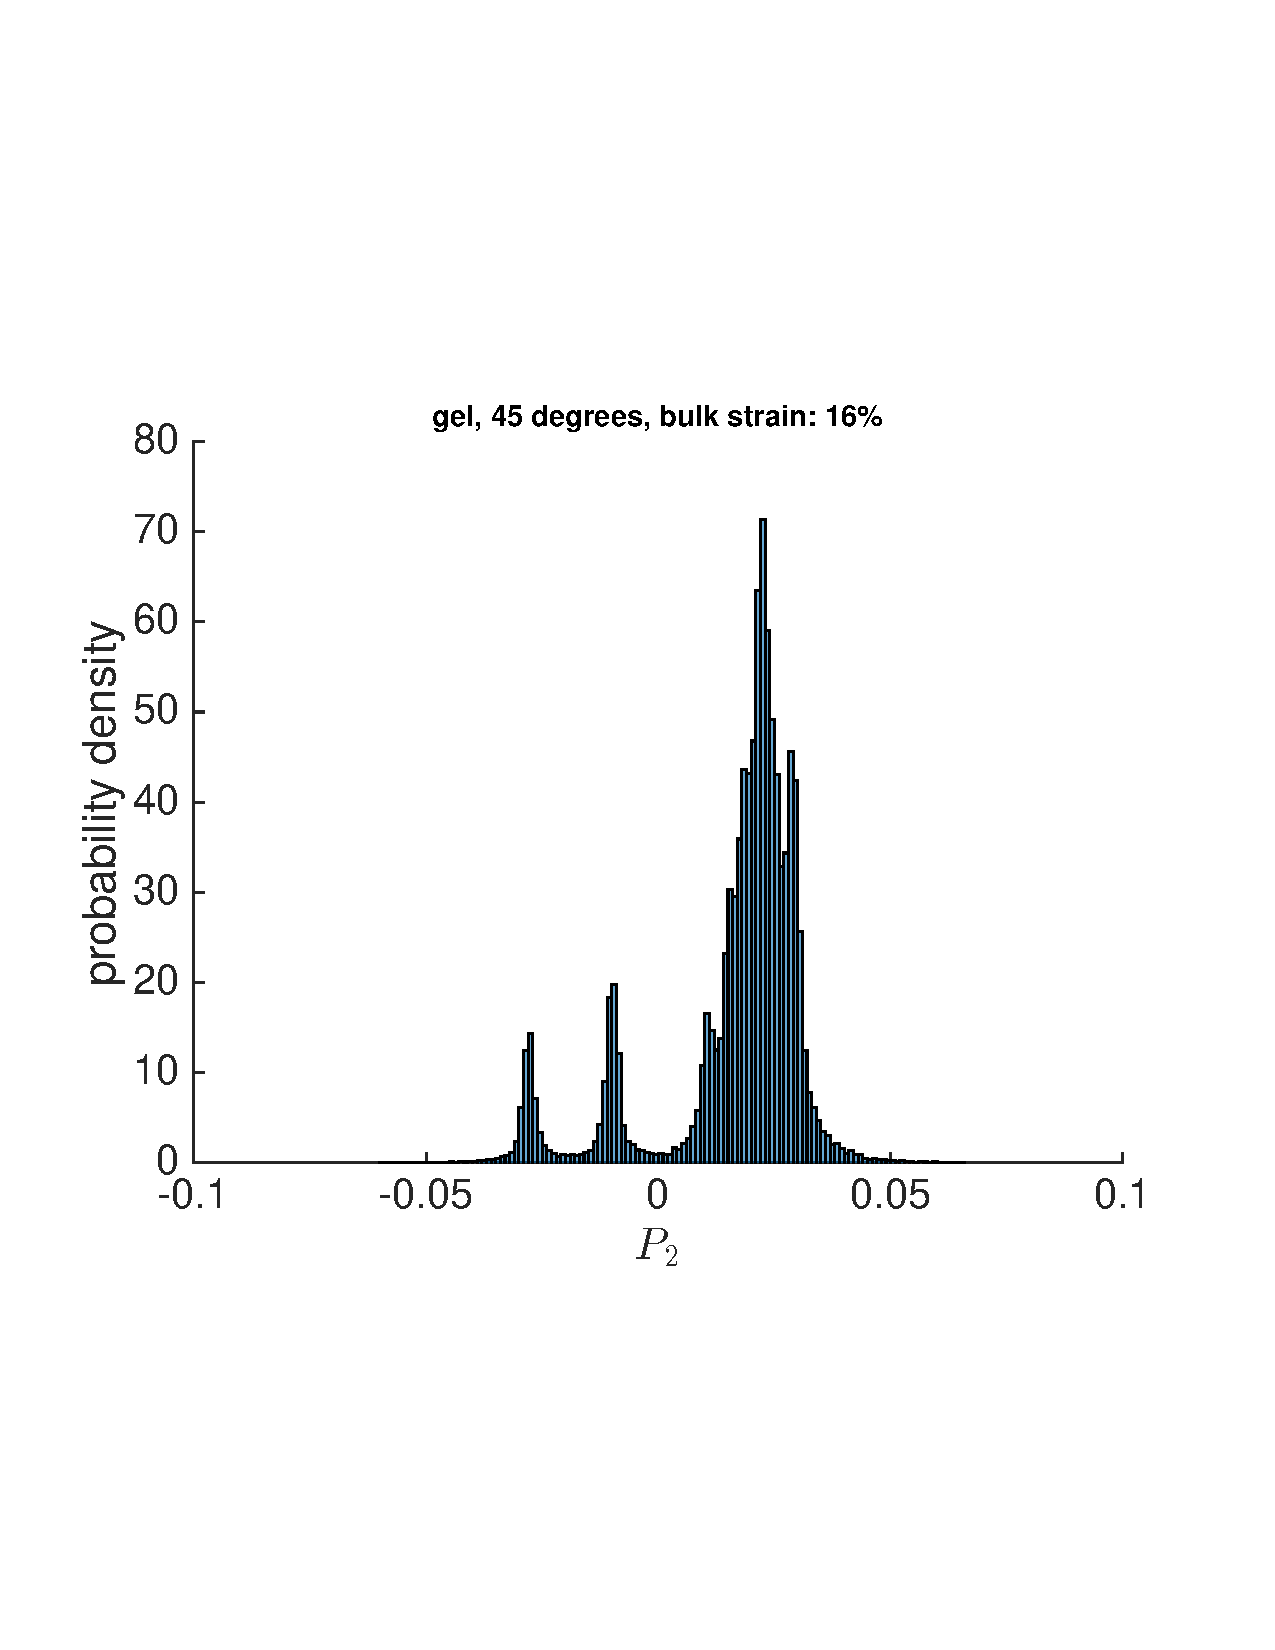
\includegraphics[height=4cm]{figure/rot45_FT50_128_1920_histo_gel_20.pdf} &
%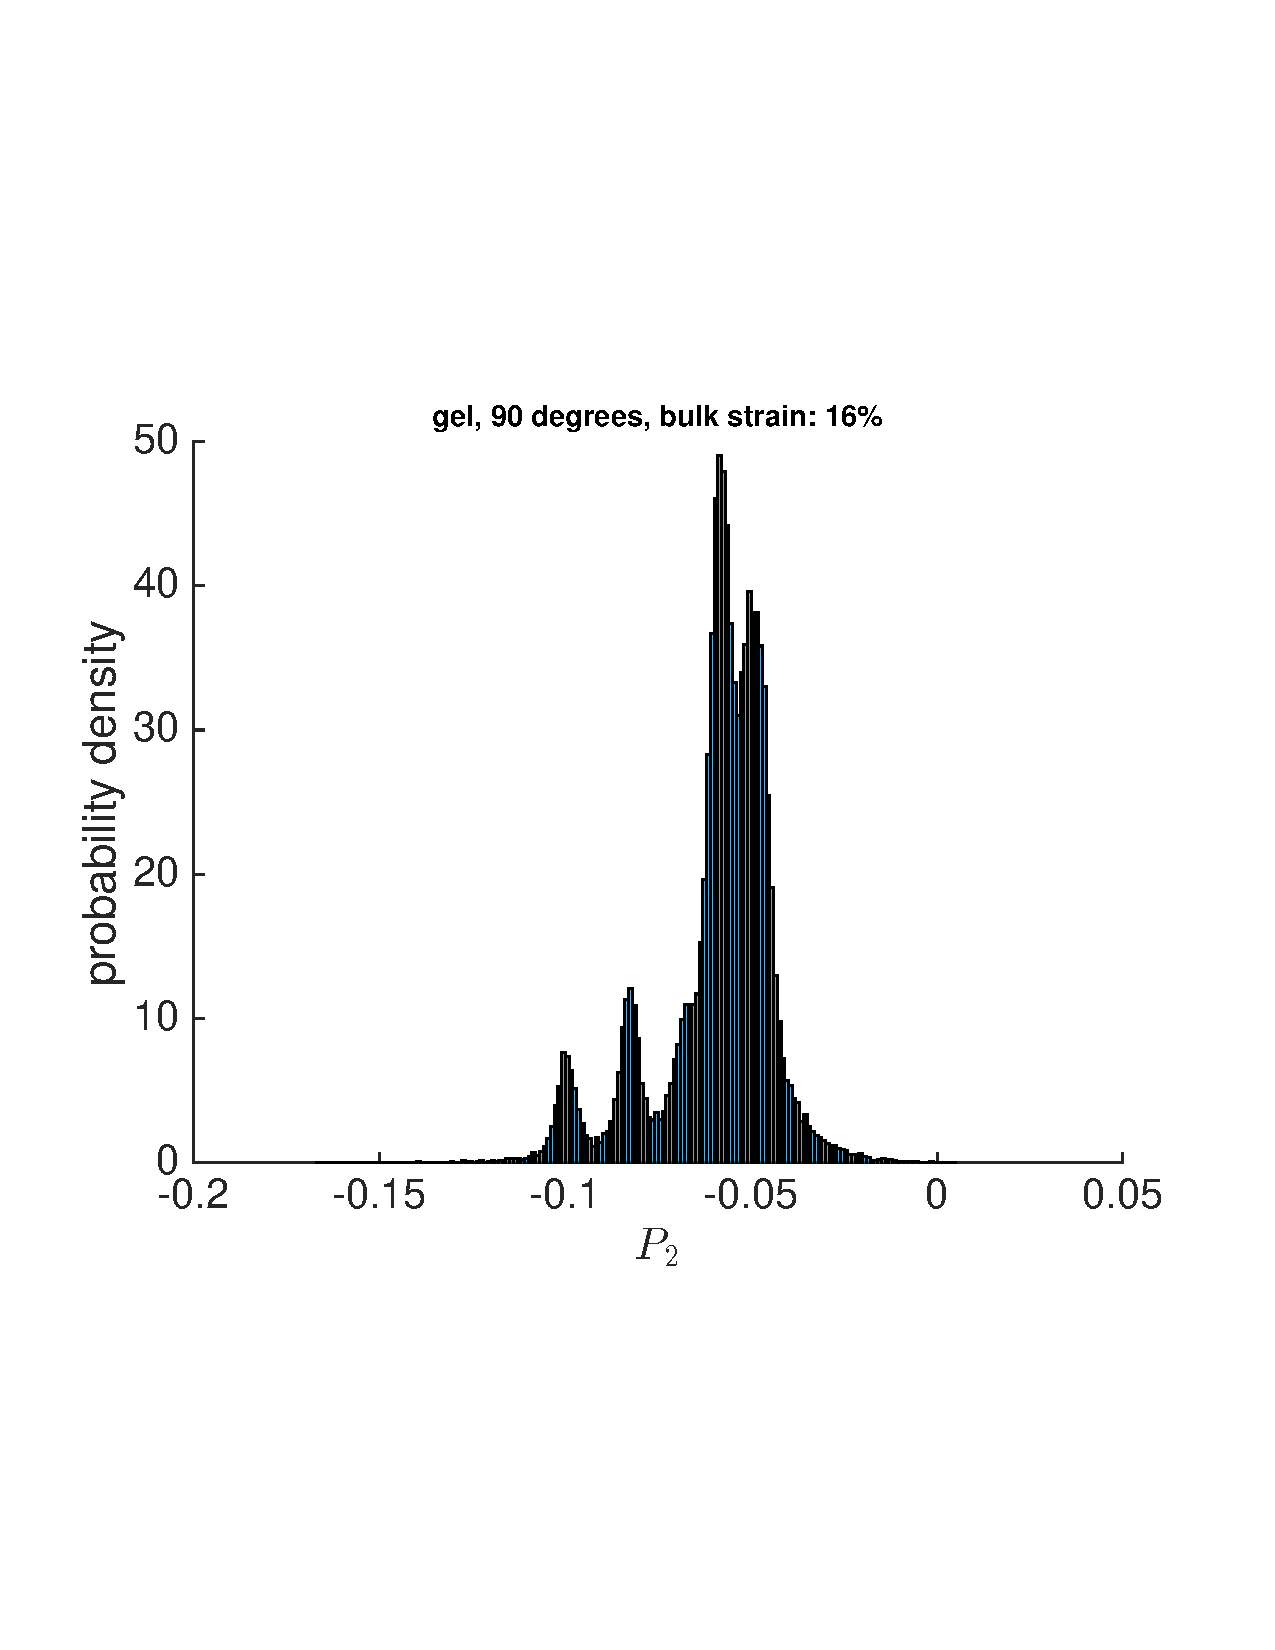
\includegraphics[height=4cm]{figure/rot90_FT_dspBC50_a30_128_1920_histo_gel_47.pdf} \\
%(d) & (e) & (f)
%\end{array}
%$
%\end{center}
%\caption{\label{fig:gel_P2} Distribution of $P_2$ in collagen gel for applied loads at 0 degrees (left column), 45 degrees (middle column), and 90 degrees (right column). The distributions for 10$\%$ (top row) and 16$\%$ (bottom row) bulk strain are shown. $P_2$ is calculated relative to the [1,0,0] axis, i.e., the axis along the direction of 0 degrees applied load.}
%\end{figure}
%%
%
%%
%\begin{figure}[ht]
%\begin{center}
%$
%\begin{array}{c}
%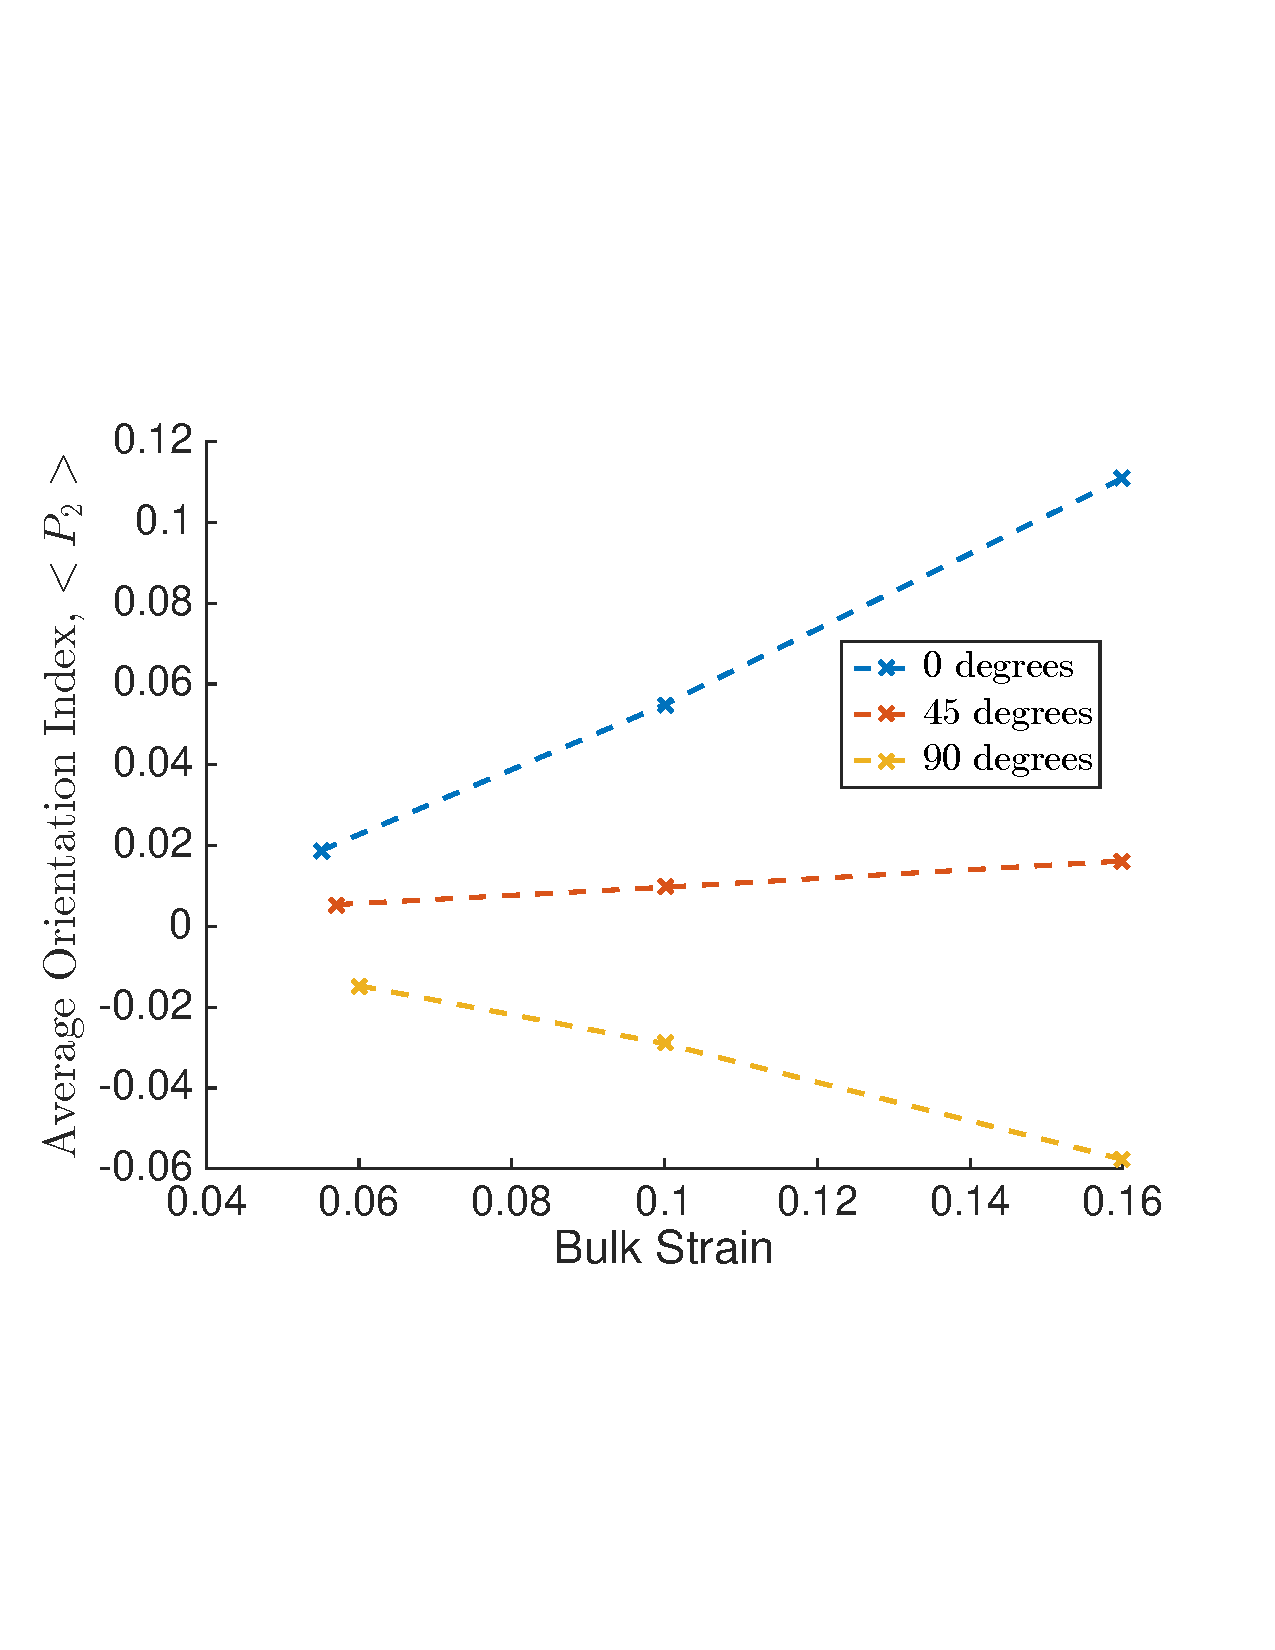
\includegraphics[height=6cm]{figure/avgP2.pdf} 
%\end{array}
%$
%\end{center}
%\caption{\label{fig:avg_P2} Average of $P_2$ in the gel for applied loads at 0, 45, and 90 degrees. $P_2$ is calculated relative to the [1,0,0] axis, i.e., the axis along the direction of 0 degrees applied load.}
%\end{figure}
%%
%%%%%%%%%%%%%%%%%%%%%%%%%%%%%%%%%%%%%%%%%%%%%%%%%%%%%%%%%%%%%%%%%%%%%%
\section{Conclusion}

In this paper we investigated the mechanical response of a neuron that is deformed while embedded in a collagen gel. The following are the main findings of this work

\begin{enumerate}
\item For all loading conditions considered, the strain experienced in the neuron is 3 to 6 times larger than the applied (bulk) strain in the surrounding collagen gel.
\item Two contributions that arise from deforming the embedded neuron system are identified. First, the neuron structure rotates to align with the direction of loading as the collagen gel is deformed. Second, the collagen gel stiffness increases with deformation. Since the neuron is much stiffer in the axial direction, the first contribution causes the neuron to become stiffer relative to the collagen gel. On the contrary, the second contribution causes the neuron to become softer relative to the collagen gel.
\item The change in the local-strain amplification (increase or decrease) as the surrounding collagen gel deforms depends on whether the first or second contribution dominates. Physiologically, an increasing local-strain amplification (second contribution dominates) can give rise to neuronal damage under moderate loading conditions on the surrounding gel. On the contrary, a decreasing local-strain amplification (first contribution dominates) prevents neuronal damage.
\item The local-strain amplification increases with collagen gel deformation in the configuration in which the axial direction of the neuron is orthogonal (or nearly orthogonal) to the loading direction (e.g., 90 degree loading angle). 
\item The alignment of the neuron during deformation (first contribution) is due to the lateral compressive strains that arise from the Poisson effect. Therefore, the alignment of the neuron is enhanced when the Poisson ratio is larger. This suggests that the increasing Poisson ratio in the collagen gel is essential for preventing injury to the neuron.
\end{enumerate}

%%%%%%%%%%%%%%%%%%%%%%%%%%%%%%%%%%%%%%%%%%%%%%%%%%%%%%%%%%%%%%%%%%%%%%
\begin{acknowledgment}

\end{acknowledgment}

%%%%%%%%%%%%%%%%%%%%%%%%%%%%%%%%%%%%%%%%%%%%%%%%%%%%%%%%%%%%%%%%%%%%%%
% The bibliography is stored in an external database file
% in the BibTeX format (file_name.bib).  The bibliography is
% created by the following command and it will appear in this
% position in the document. You may, of course, create your
% own bibliography by using thebibliography environment as in
%
% \begin{thebibliography}{12}
% ...
% \bibitem{itemreference} D. E. Knudsen.
% {\em 1966 World Bnus Almanac.}
% {Permafrost Press, Novosibirsk.}
% ...
% \end{thebibliography}
\newpage
% Here's where you specify the bibliography style file.
% The full file name for the bibliography style file 
% used for an ASME paper is asmems4.bst.
\bibliographystyle{asmems4}

% Here's where you specify the bibliography database file.
% The full file name of the bibliography database for this
% article is asme2e.bib. The name for your database is up
% to you.
\bibliography{references}


\end{document}
